\chapter{Check of the assumptions}\label{checkass}
For the whole workflow several assumptions about the data or the results of certain transformations are made. These assumptions have to be met at least roughly to ensure the correctness of the results.\newline
This section gives checks for most of the assumptions like accuracy of the PSF scale estimation or that the matched filter of the matching size compared to the PSF performs best.\newline
Also a discussion about the design choices is present in this chapter.
\section{Calibration measurement}
As described by \cite{meanVar} the gain can be determined using the mean and variance of data with different mean intensities. Therefore a calibration dataset was acquired. The temperature and the gain factor were set to match the settings usually used. A sample with cells was prepared for the Storm measurement. First, eleven time series were taken, with open shutter and with increasing exposure time from 0 milliseconds up to 1000 milliseconds. Afterwards the same procedure was repeated with the shutter closed. Figure \ref{calibplot} shows the results for the first 6 exposure times. All points lie on a straight line. The gain factor determined by the calibration measurement was 3.9, the offset 315. This offset is too small which was found out by comparing the offset to the intensities from closed shutter measurements. Another method was used to determine the offset. There were also another series of images taken with closed shutter. This series shows the response of the camera without any light entering the camera. The mean value of the shortest exposure time was taken as offset. Its value is 380. 
\begin{figure}[H]
\centering
\includegraphics[width = 0.465\textwidth]{pictures/meanVariancePlotCalibrationgimp.png}
	 \caption{Result of the calibration measurements. The gain determined from this variance-mean plot is 3.9.}
	\label{calibplot}
\end{figure}


\section{Correction to Poisson distributions}
It is very important for the whole workflow that the first transform results in background intensities that follow a Poisson distribution. To test this, a real world image was transformed with parameters taken from the calibration measurement described above. The offset was estimated from the minimal intensity of the raw image. The histograms for two generic background pixels are shown in Figure \ref{isitPoisson}. A Poisson distribution with the mean of the pixels intensities is also shown in the figures. These histograms were acquired using the pixel intensities of one pixel for 3000 frames. The histogram matches the expected Poisson distribution.
\begin{figure}
\subfloat[Tubulin2 frame 10]{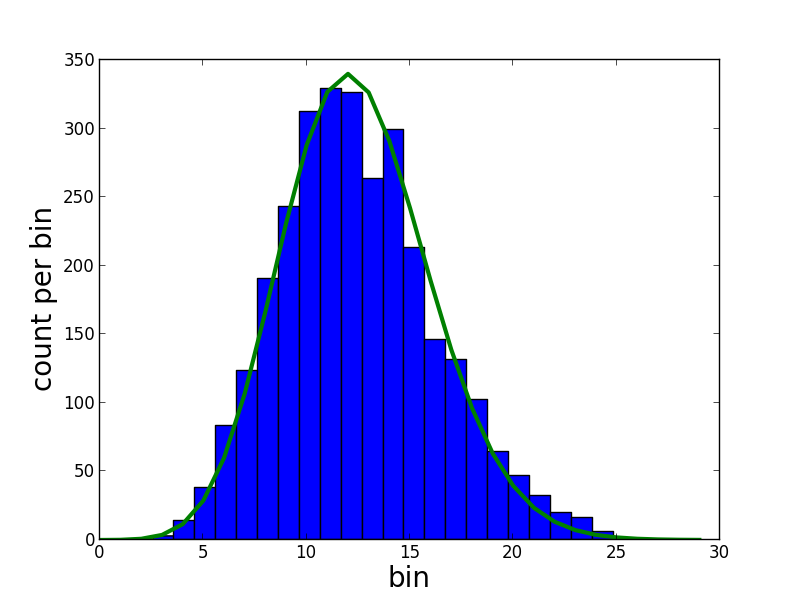
\includegraphics[width = 0.485\textwidth]{pictures/IsItPoisson105_105.png}}\hfill
\subfloat[Tubulin2 frame 1010]{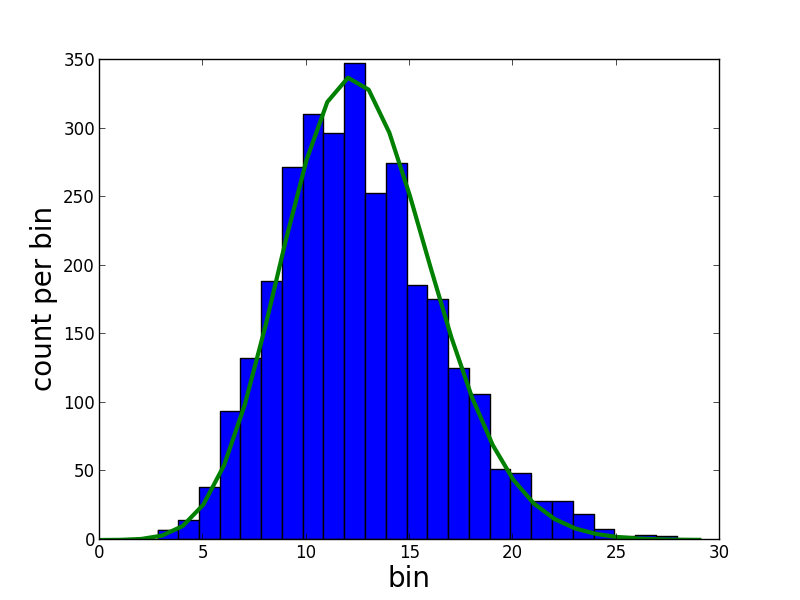
\includegraphics[width = 0.485\textwidth]{pictures/IsItPoisson50_50.png}}
	\caption{These pictures show how well the histograms of background pixels taken over the first 3000 frames, follow a Poisson distribution. For the gain the parameter from the calibration measurement of $g$ = 3.9 was used. The offset was estimated from the minimal intensities of the original image.}
	\label{isitPoisson}	
\end{figure}

\section{Result Anscombe transformation}
After the transformation described in section \ref{trafoPoiss}, the Anscombe transformation was applied to the same data set that was used in the previous section and the background was subtracted. Figure \ref{isitAnscombe} shows the histogram of the intensities of one randomly chosen frame and a Gaussian with zero mean and unit variance. The histogram fits very well to the Gaussian. The tail exceeding the Gaussian on the right side can be explained by the signal that is present in the image and does not follow the Gaussian distribution, but has higher intensities.\newline
\begin{figure}
\centering
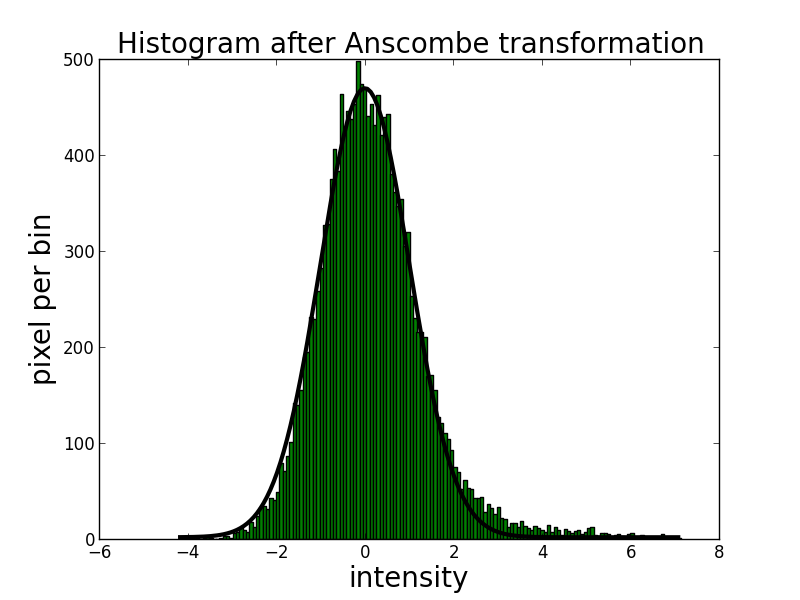
\includegraphics[width = 0.485\textwidth]{pictures/anscombeAndFit.png}
	 \caption{After the Anscombe transformation the background pixel intensities should be distributed with mean zero and variance one. This Figure shows the histogram of the pixel intensities and a fitted Gaussian with variance one and mean zero.}
	\label{isitAnscombe}
\end{figure}
There may be confusion why the Anscombe transformation that is applied to all intensities of one time step instead of all intensities of one pixel, does work. This is because the Anscombe transformation is applied to each intensity independently. Therefore all intensities at a certain time step are one sample from the Gaussian distribution in $t$ dimension that results from the Anscombe transformation. All of these Gaussian distributions in $t$ dimension have the same mean (since the background was subtracted) and variance (unit variance since Anscombe transformation). This means that the distribution created from all intensities of a certain frame has the same mean and variance as the transformed Poisson distributions in $t$ dimension.
\section{Accuracy of detection}
Unfortunately the position of the fluorescent molecules can not be detected
perfectly. There are two main contributions to the error in detection.\\
On one hand, there is a problem with finding the maximum in a noisy signal. Due to
noise the spots maxima might be shifted.\newline
On the other hand, the position of the fluorescent molecule is detected by upscaling the pixel grid and interpolation.
After that the maximums position of the upscaled grid is taken as the resulting
position. This gives an error from roughly a 12th pixel width. This error becomes less important with higher upscaling factors.\newline

Because there is no groundtruth for the real data, test data and groundtruth had to be produce. This was done similar to the method described by \cite{simulated}. The difference was that, instead of generating only one spot per frame a different number of spots were simulated for each frame. For different signal-to -noise ratios, a dataset with 40 times 40 pixels and 1000 frames was created. Each frame containing one, three or five point spread functions. The same spots were used for each SNR.\newline

To determine the accuracy, the standard deviation between the true position of the signal and its detection were used. For data sets with more than one spot per frame, the best match within a certain distance around the true position was found. If a pair of true spot and detection were found, both were removed for further matching of the remaining signals. In the end the averaged standard deviation of the detection relative to the true positions were calculated as follows:
\begin{align}
	\text{std. dev.} = \sum_i^{\#\text{ pairs}} \sqrt{\left(\bf{p}_{\text{true}}^i - \bf{p}_{\text{detec}}^i\right)^2}
\end{align}
$i$ runs over all found pairs of groundtruth and detections, $\bf{p}$ describes the two dimensional spatial vector of the groundtruth or detection respectively. False detections with no corresponding spot in the groundtruth did not contribute to the localization error.\newline

The results can be seen in Figure \ref{accplot}. The Figure shows that the more spots are present per frame the harder it is to detect them properly. This is a result of the fact that spots that lay near each other might be detected as one spot. This gives rise to higher errors in the detection accuracy.


\begin{figure}
\begin{minipage}[t]{0.48\textwidth}
\includegraphics[width = 0.99\textwidth]{pictures/AccuracyTest2.png}
	\caption{Result of the accuracy test. For datasets with one, three or five point spread functions per frame, evaluated for different signal to noise levels. The more dense the spots are the less accurate the detections are. The PSFs standard deviation is 1.4.}
	\label{accplot}	
\end{minipage}\hfill
\begin{minipage}[t]{0.48\textwidth}
\centering
\includegraphics[width = 0.99\textwidth]{pictures/AccuracyTestSigma2.png}
	\caption{Result of the accuracy test for different sigmas for the Gaussian smoothing. One data set was processed with different sigma values and evaluated for different signal to noise levels. The true standard deviation of point spread function of the simulated data is 1.4.}
	\label{accplot2}

\end{minipage}
\end{figure}


\section{Matched filter is best filter} \label{detectionError}
For denoising the image a matched filter is used. Since it is assumed that the point spread function is Gaussian, a two dimensional Gaussian filter with the estimated size of the point spread function is used. The following calculation shows why this is the best choice for the standard deviation.\newline
This calculation was inspired by the calculation in \cite{ulli}, page 207.\newline 
The assumptions are: the point spread function is Gaussian shaped with a true standard deviation of $\sigma_\text{PSF}$, the image contains white Gaussian noise with mean zero and unit variance, the applied filter for denoising is a Gaussian filter with standard deviation $\sigma_\text{filter}$.\newline
The image $f$ is composed of Gaussian filtered signal $s$ and white noise $n$ mentioned above. $s$ and $n$ describe the filtered signal respectively noise.
\begin{align}
 f=s+n \label{gl91}
\end{align}
Without noise the first derivative of $f$, which is equal to $s$ in the noise-free case, vanishes at the center of the Gaussian signal. This center can be set to the origin without losing generality. But noise shifts the zero crossing of the first derivatives to $\Delta x,~\Delta y$. For now only one dimension is considered.
\begin{align}
\frac{\partial f}{\partial x}\left(\Delta x, \Delta y\right) &= \frac{\partial s}{\partial x} \left(\Delta x, \Delta y\right) + \frac{\partial n}{\partial x}\left(\Delta x, \Delta y\right)&=0
\end{align}  

Using Taylor expansion around $x = 0$ at $y= 0$ for the signal, yields:
\begin{align}
f_x(\Delta x, \Delta y)&\approx \underbrace{s_x(0, 0)}_{=0} + s_{xx}(0, 0)\cdot \Delta x + n_x(\Delta x, \Delta y)&=0\\
\Rightarrow \text{var}(s_{xx}(0, 0)\cdot \Delta x)&= \text{var}(n_x(\Delta x,\Delta y)\\
\Rightarrow \text{var}(\Delta x) &= \frac{\text{var}(n_x(\Delta x, \Delta y)}{s_{xx}^2(0, 0)} \label{ch9gl1}
\end{align}

The result for the variance of the first derivative of white noise convolved with a Gaussian filter of width $\sigma_\text{filter}$ can be found at \cite{ulli}, page 204. It is:
\begin{align}
	\text{var}(n_x) = \frac{N^2}{8\pi\sigma_\text{filter}^4},~\text{with }N\text{: noise std. dev} \label{ch9gl2}
\end{align}
The convolution of the Gaussian PSF  with another Gaussian results in Gaussian with combined scales.
\begin{align}
 \mathcal{N}(0,\sigma_\text{PSF}) \ast \mathcal{N}(0,\sigma_\text{filter}) = \mathcal{N}\left(0,\underbrace{\sqrt{\sigma_\text{PSF}^2+\sigma_\text{filter}^2}}_{=\sigma_\text{comb}}\right)
\end{align}
The value of the second derivative in $x$-direction of the convolved PSF at (0,0) is:
\begin{align}
 \frac{\partial^2 S_0\cdot\mathcal{N}\left((\mu_x,\mu_y),\sigma_\text{comb}\right)}{\partial x^2}  &=  -\frac{S_0}{2\pi \sigma_\text{comb}^4}  \label{ch9gl3}
\end{align}
Combining equations \ref{ch9gl1}, \ref{ch9gl2} and \ref{ch9gl3} yields:
\begin{align}
\text{var}\left(\Delta x\right) &= \dfrac{\dfrac{N^2}{8\pi\sigma_\text{filter}^4}}{\dfrac{S_0^2}{4\pi^2 \sigma_\text{comb}^8}}\\
&= \frac{N^2\cdot 4\pi^2 \sigma_\text{comb}^8}{S_0^2\cdot8\pi\sigma_\text{filter}^4}\\
&= \frac{N^2}{S_0^2} \frac{\pi \left(\sigma_\text{filter}^2+\sigma_\text{PSF}^2\right)^4}{2\sigma_\text{filter}^4}\\
&= \frac{N^2\pi}{2S_0^2} \left(1+\frac{\sigma_\text{PSF}^2}{\sigma_\text{filter}^2}\right)^2\left(\sigma_\text{filter}^2+\sigma_\text{PSF}^2\right)^2 
\end{align}
The same calculation can be done with respect to $y$. This gives the same variance, yielding a total variance that is square root of 2 times larger, because the variances are orthogonal.
Therefore the standard deviation of the localization is:
\begin{align}
 \text{std. dev loc}&=\frac{N}{S_0}\sqrt{\frac{\sqrt{2}\pi}{2}}
 \left(1+\frac{\sigma_\text{PSF}^2}{\sigma_\text{filter}^2}\right)\left(\sigma_\text{filter}^2+\sigma_\text{PSF}^2\right) 
\end{align}
To verify these results test data sets have been created containing 3500 frames with one PSF per frame. Each created data set contained a PSF with different scale. This data sets have been filtered with Gaussian filters of different sizes. After that the maximum for each frame was detected and compared with the true position. Figure~\ref{matchedFilter1} shows the accuracy for different PSF scales and filter widths.\newline
The best results were achieved using a Gaussian filter with the PSFs size. The larger the PSFs scale the more inaccurate the localization becomes.\newline

\begin{figure}
\centering
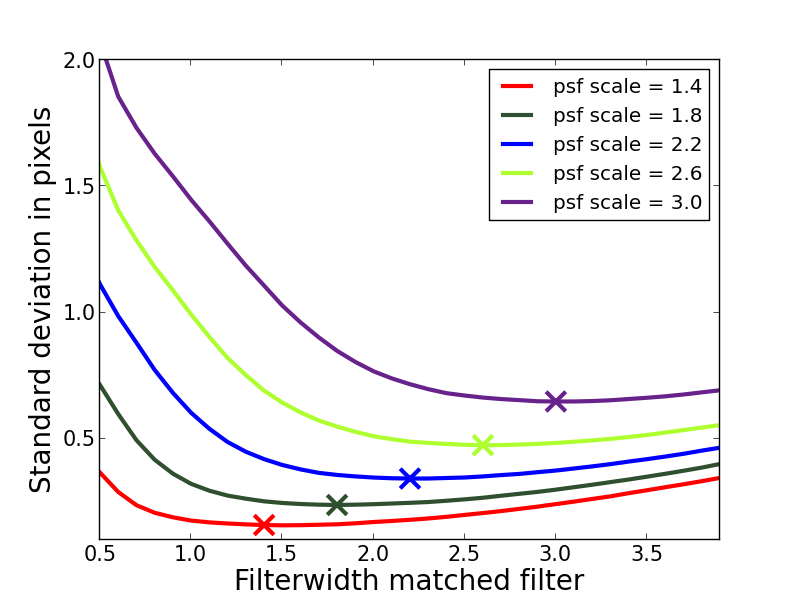
\includegraphics[width = 0.485\textwidth]{pictures/matchedFilterPlots1.png}
	 \caption{This Figure shows the accuracy of detection achieved using different Gaussian filters for denoising. The cross marks the minimum of each curve.}
	\label{matchedFilter1}
\end{figure}

The Figures in \ref{matchedFilter2} show the measurement, a shifted measurement curve and the result of the calculation. The measured error was larger than the calculated error, therefore the shifted line is also shown to state that the curves shape match but there is an additional error that shifts the line. \newline
These results show that the calculated standard deviation of the localization can be used to estimate the localization error of SimpleSTORM for further calculations or error propagation.\newline

\begin{figure}
\centering
\subfloat[PSFs scale = 2.6]{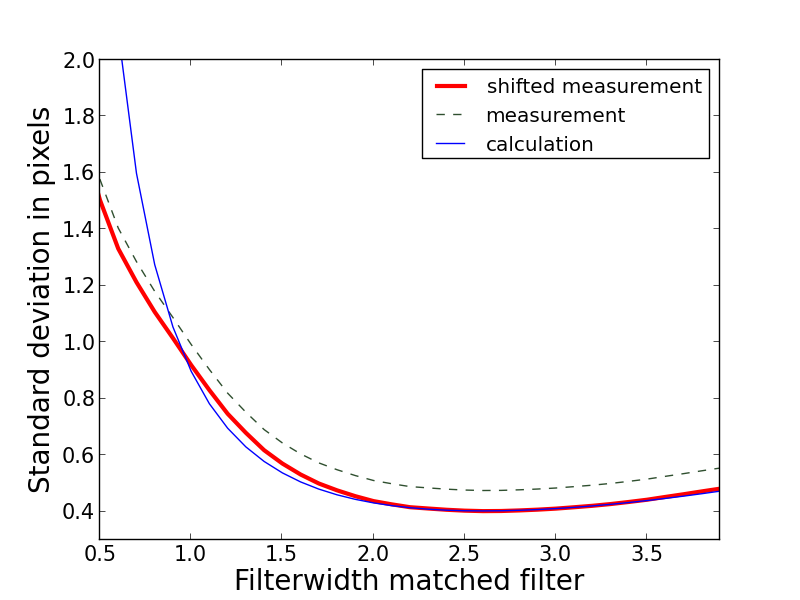
\includegraphics[width = 0.485\textwidth]{pictures/matchedFilterPlots2.png}}\hfill
\subfloat[PSFs scale = 1.8]{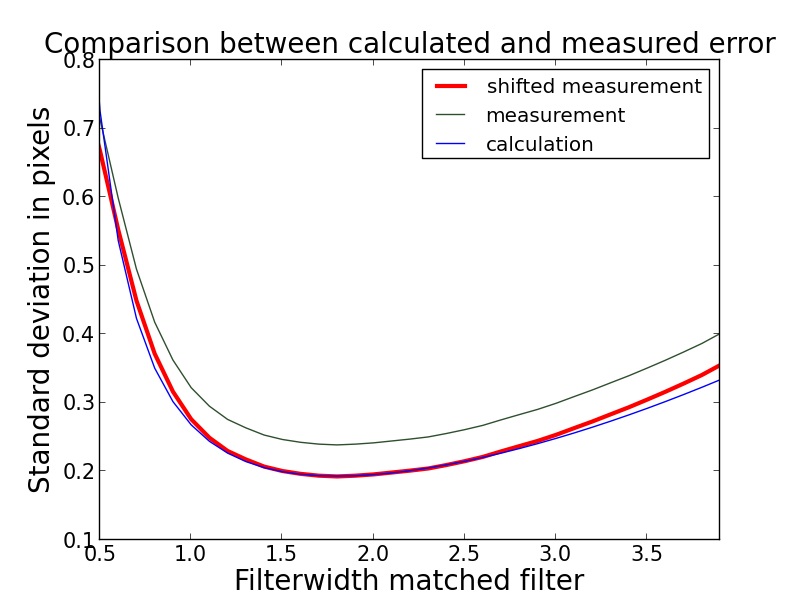
\includegraphics[width = 0.485\textwidth]{pictures/matchedFilterPlots3.png}}
	\caption{Comparison between the measured and the calculated localization error. The dashed lines show the unchanged measurement results, for better comparison the line was shifted to match the calculated error.}
	\label{matchedFilter2}	
\end{figure}
It is important that the size of the ideal filter does not depend on whether an Anscombe transformation is applied to the data or not. The Anscombe transformation increases the standard deviation of the PSFs, this is shown in the next section. However the filter width that gives the lowest error is the original width of the PSF. This is shown in Figure \ref{PSFdoesnotcare}. A data set with 3500 frames and a PSF with $\sigma=1.5$ was created. Then the Anscombe transformation is applied to one copy of the data set. Both data sets were filtered with filters of different scale. The localization error is then plotted over the used filter scale.

\begin{figure}
\centering
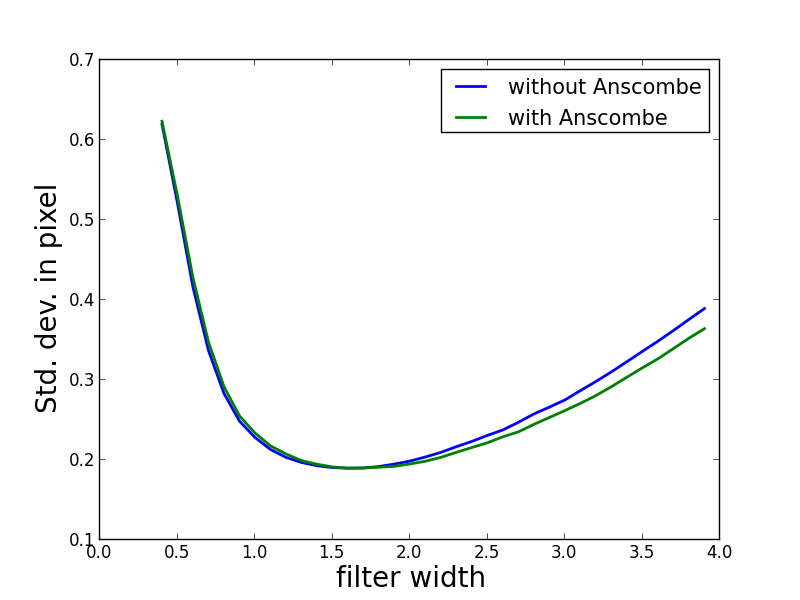
\includegraphics[width = 0.5\textwidth]{pictures/AnscVsNoAnsc.png}
\caption{This plot shows the influence of the Anscombe transformation on the localization error for a PSF with $\sigma=1.5$, which was filtered with Gaussian filters of different size. It can be seen, that the minimum of the localization error is the same for data with applied Anscombe transformation and for data without.}
\label{PSFdoesnotcare}
\end{figure}

\section{Influence of Anscombe transformation on the PSF}\label{PSF}
The Anscombe transformation has no influence on the best matched filter, however the standard deviation of a PSF after applied Anscombe transformation changes compared to the original standard deviation. This change in the standard deviation depends on the SNR of the PSF. Figure \ref{psfwider} shows the change of the standard deviation of a PSF with $\sigma=1$ for different SNRs. To avoid estimating a mean SNR for all PSFs used to calculate the mean power spectrum, an inverse Anscombe transformation is applied before the Fourier transform is applied.\newline
The reason why the inverse Anscombe transformation is used instead of not applying the Anscombe transformation, is that the data processing part is the same for all parts of the program (transformation to Poisson distributed background, background estimation and subtraction, Anscombe transformation). Therefore it is easier to do the inverse transformation instead of changing the data processing part.

\begin{figure}
\centering
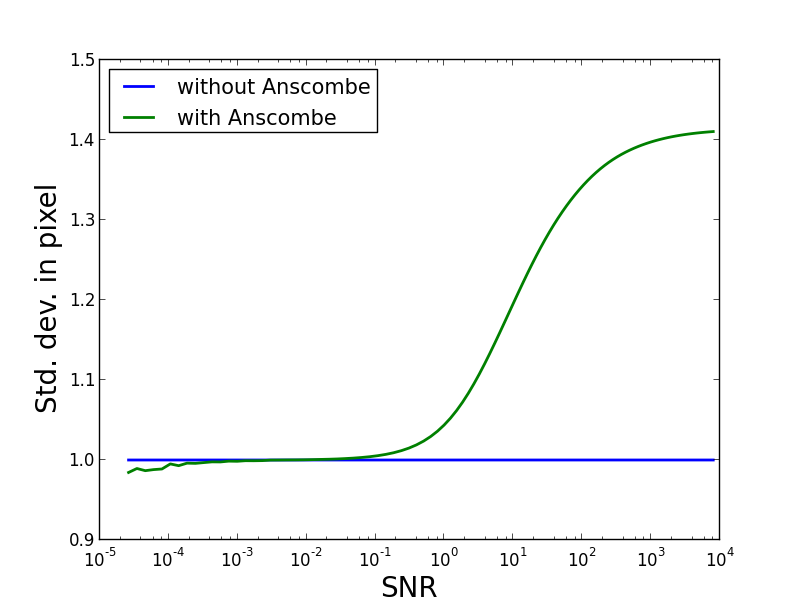
\includegraphics[width = 0.485\textwidth]{pictures/AnscombeChangesWidth.png}
\caption{The standard deviation of the Anscombe transformed PSF changes with respect to the SNR.}
\label{psfwider}
\end{figure}

\section{Test PSF estimation}
The estimation of the width of the point spread function of the signal is very important. The localization error increases with larger deviations of the matched filters width from the true width of the PSF, as shown in section \ref{detectionError}. \newline
Figure \ref{estimatedSigma} shows the results of an accuracy test. For this test, data was created artificially. One PSF was simulated at a random location with a fixed width, Poisson noise was added. The signal-to-noise ratio was set to 10. Then the width of the PSF was estimated by the SimpleSTORM algorithm. This was done with values for the standard deviation of the Gaussian in a range from 0.2 up to 4. The plot shows that for standard deviations up to 2.5 the estimated value for the width is very close to the actual value. The wider the PSF becomes in the spatial domain the smaller it gets in the Fourier domain. This is why the accuracy of estimation decreases for larger widths. Choosing a larger region of interest for the power spectrums accumulation reduces this effect. The parameter chosen for the region of interest for the plot in figure \ref{estimatedSigma} was the default value. The typical width of the PSF for real world data is in a range of 1 to 2, in which the estimation gives reliable results.\newline
%\begin{figure}
%\centering
%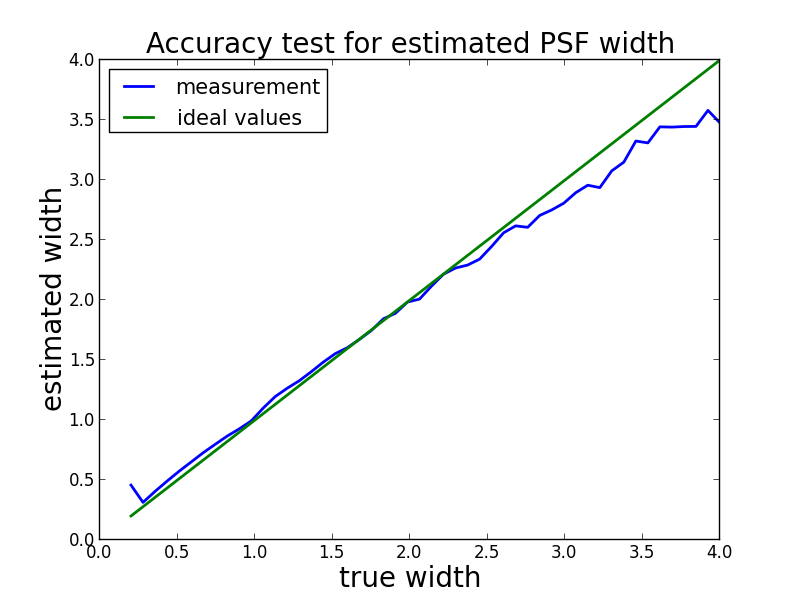
\includegraphics[width = 0.485\textwidth]{pictures/AccuracyTestPSFWidth.png}
%	 \caption{The figure shows the estimated widths of the point spread function plotted over the true %width of the simulated signal. The signal-to-noise ratio was 10 for this test. The green line shows the %simulated values.}
%	\label{estimatedSigma}
%\end{figure}


\section{Bleaching signal}
One assumption was that the backgrounds illumination is caused mainly from out of focus fluorophors and is therefore Poisson distributed. If this is the case the background illumination should decrease over time. Bleaching of fluorophores describes the process in which the fluorescent molecules change their conformation and lose the ability to emit light permanently. The spectrum of the emission can also change so that the fluorescent molecules can not be detected any more. All fluorophores used for the STORM images available bleach over time. The decay of the mean background intensity is shown in Figure \ref{bleaching}.

%\begin{figure}
%\centering
%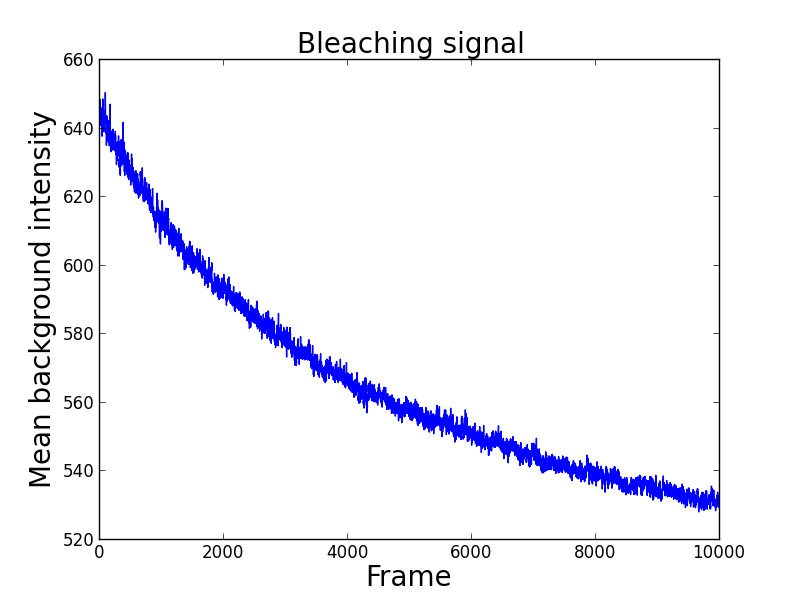
\includegraphics[width = 0.485\textwidth]{pictures/bleaching.png}
%	\caption{The number of active fluorophores decreases over time and so does the mean intensity of the %image. This picture shows the mean intensities of 10 background pixel over time. }
%	\label{bleaching}
%\end{figure}

\begin{minipage}[t]{0.45\textwidth}
\includegraphics[width = \textwidth]{pictures/AccuracyTestPSFWidthgimp.png}
\captionof{figure}{The figure shows the estimated widths of the point spread function plotted over the true width of the simulated signal. The signal-to-noise ratio was 10 for this test. The green line shows the simulated values.}\label{estimatedSigma}
\end{minipage}
\hfill
\begin{minipage}[t]{0.45\textwidth}
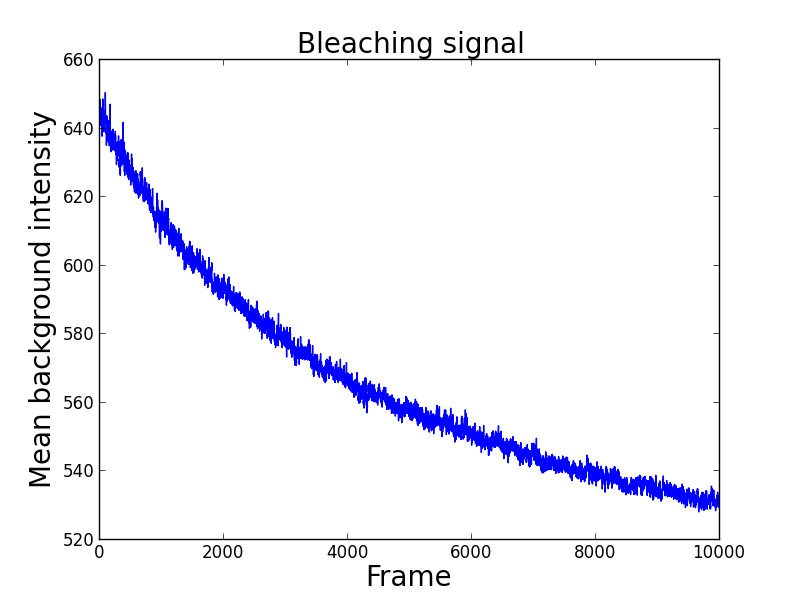
\includegraphics[width = \textwidth]{pictures/bleaching.png}
\captionof{figure}{The number of active fluorophores decreases over time and so does the mean intensity of the image. This picture shows the mean intensities of 10 background pixel over time.}\label{bleaching}
\end{minipage}

\section{Reliability of skewness estimation} \label{skewnesssucks}
To estimate the true Poisson distributions mean using its skewness is a direct way to get to the true distributions mean regardless of the camera parameters.\newline
This approach has one drawback. The larger the mean value of a Poisson distribution becomes, the more similar the Poisson distribution becomes to a Gaussian. This means that the skewness, which measures the asymmetry of the distribution becomes smaller and smaller, converging to zero. The inverse of the skewness squared is used to estimate the mean of the Poisson distribution, this means that small uncertainties for the skewness lead to a high uncertainty for the estimated mean. Also a single distribution with a couple of hundred samples yields no reliable estimate. A robust estimate can be achieved if the median of the estimated mean of several distributions is calculated. Figure \ref{skew1000} shows the results of the estimate of the mean using the skewness approach on patches of different size. The plot shows the estimated value on the ordinate, the true value on the abscissa. The different lines show the results for different sizes of the distribution. Figure \ref{skew100} shows the same plot but for smaller distribution sizes. It can be seen, that the more pixels are used and the more samples are available, the better the estimate becomes.

\begin{figure}
\subfloat[10 times 10 pixel patch]{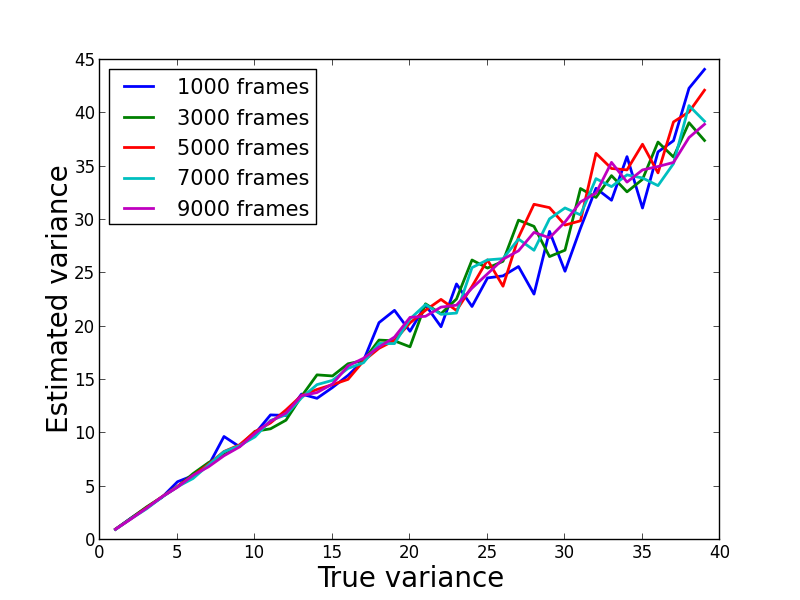
\includegraphics[width = 0.485\textwidth]{pictures/skewness100.png}}\hfill
\subfloat[20 times 20 pixel patch]{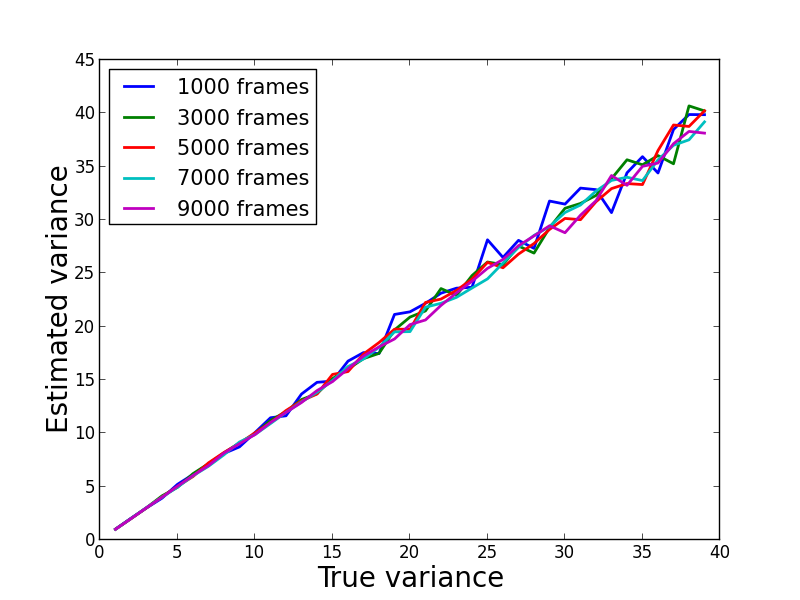
\includegraphics[width = 0.485\textwidth]{pictures/skewness400.png}}
	\caption{Result of mean estimation using skewness approach.}
	\label{skew1000}	
\end{figure}
\begin{figure}
\subfloat[10 times 10 pixel patch]{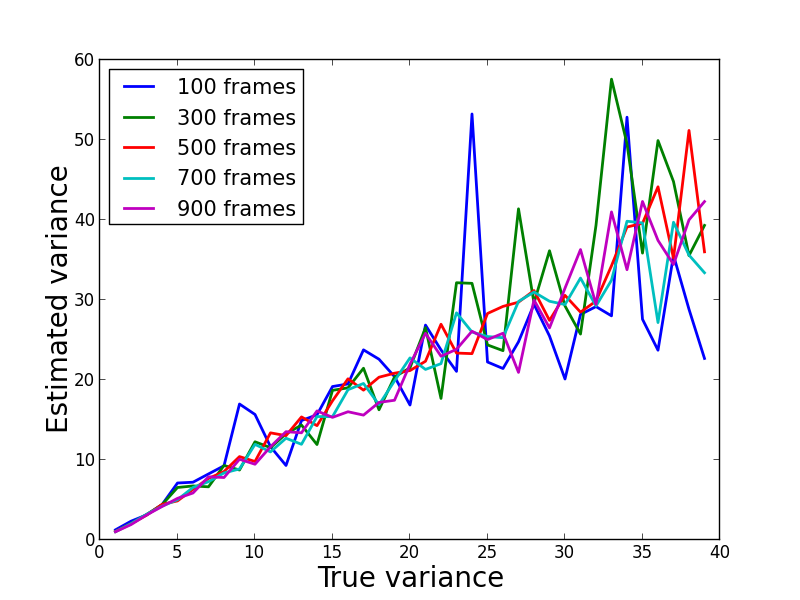
\includegraphics[width = 0.485\textwidth]{pictures/skewness2100.png}}\hfill
\subfloat[20 times 20 pixel patch]{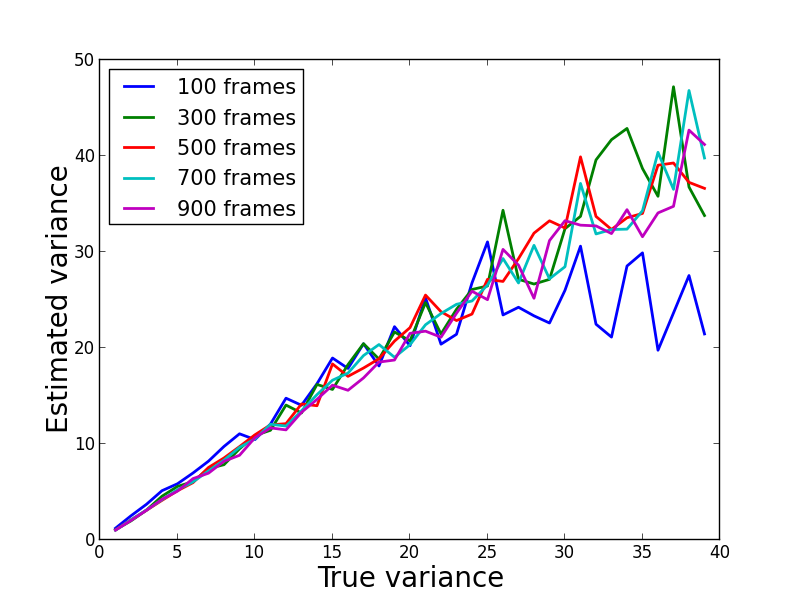
\includegraphics[width = 0.485\textwidth]{pictures/skewness2400.png}}
	\caption{Result of mean estimation using skewness approach.}
	\label{skew100}	
\end{figure}
The estimate for the mean is accurate even for a smaller number of samples up to 15 to 20.\newline
This approach has the drawback that for small data sets with only several hundred frames the accuracy of the estimated values is low. Another problem is artificially created data sets with a background intensity of 100 or above. In that case the skewness approach gives no reliable results.

\section{Points lie on or above the desired line}\label{pointsabove}
To estimate the camera gain and offset from the raw data the method described in section \ref{skellam1} is used. Ideally the intensities for every pixel would follow a Poisson distribution with a certain mean. However this assumption only holds for beads and background pixel that never is affected by signal. The resulting points in the variance over mean plot will lie on a straight line. But what happens if background pixels are illuminated by a fluorophore in one or several frames?\newline
This section proves that points in the variance over mean intensity plot lie on the straight line or above, but almost never below.\newline
Set $A$ contains $n$ samples drawn from a Poisson distribution. The variance and mean of the set shall be $\mu_p$. Set $B$ is equal to set $A$ but the last ($n^\text{th}$) member $p_n^A$ is replaced by $p_n^A+c$. $c$ is a positive value that describes the difference in intensity between a background pixel and an illuminated pixel. This models the additional intensity caused by a blinking fluorophore. \newline  

The exchange of the last pixel increases the mean intensity:
\begin{align}
\mu_B&=\frac{1}{n}\sum_{i=1}^n(p_i^B)\\
&=\frac{1}{n}\left(\sum_{i=1}^{n-1}(p_i^A) +p_n^A+c \right)\\
&=\frac{1}{n}\left(\sum_{i=1}^{n}(p_i^A) +c \right)\\
&=\mu_p + \frac{c}{n}
\end{align}
The variance of set $B$ times $(n-1)$ is given as:
\begin{align}
(n-1)\cdot\text{var}(B)&=\sum_{i=1}^n \left(p_i^B - \left(\mu_p+\frac{c}{n}\right)\right)^2\\
&=\sum_{i=1}^n \left(\left(p_i^B\right)^2 - 2p_i^B\mu_p-\frac{2p_i^Bc}{n}+\left(\mu_p+\frac{c}{n}\right)^2\right)\\
&=\sum_{i=1}^n \left(\left(p_i^B\right)^2 - 2p_i^B\mu_p+\mu_p^2\right)+\sum_{i=1}^n \left(-\frac{2p_i^Bc}{n}+\frac{2c\mu_p}{n}+\frac{c^2}{n^2}\right)
\end{align}
\begin{align}
(n-1)\cdot\text{var}(B)&=\sum_{i=1}^{n-1} \Big(\underbrace{\left(p_i^A\right)^2}_{=p_i^B \text{for } i\neq n} - 2p_i^A\mu_p+\mu_p^2\Big)+\underbrace{\left(p_n^A+c\right)^2}_{=\left(p_n^B\right)^2} -2\left(p_n^A+c\right)\mu_p + \mu_p^2 \\
&~~~+\sum_{i=1}^n\left(-\frac{2p_i^Bc}{n}+\frac{2c\mu_p}{n}+\frac{c^2}{n^2}\right) \nonumber\\
&=\sum_{i=1}^{n} \left(\left(p_i^A\right)^2 - 2p_i^A\mu_p+\mu_p^2\right)+2p_n^Ac+c^2-2c\mu_p\\
&~~~+\sum_{i=1}^n\left(-\frac{2p_i^Bc}{n}+\frac{2c\mu_p}{n}+\frac{c^2}{n^2}\right) \nonumber\\
%&=(n-1)\mu_p+2p_n^Ac+c^2-2c\mu_p+\sum_{i=1}^n\left(-\frac{2p_i^Bc}{n}+\frac{2c\mu_p}{n}+\frac{c^2}{n^2}\right)\\
&=(n-1)\mu_p+2p_n^Ac+c^2+\frac{c^2}{n}-\sum_{i=1}^n\frac{2\left(p_i^B\right)c}{n}\\
&=(n-1)\mu_p+2p_n^Ac+c^2+\frac{c^2}{n}-\sum_{i=1}^{n-1}\frac{2\left(p_i^A\right)c}{n} -\frac{2\left(p_n^A+c\right)c}{n}\\
&=(n-1)\mu_p+2p_n^Ac+c^2+\frac{c^2}{n}-\sum_{i=1}^{n}\frac{2\left(p_i^A\right)c}{n} -\frac{2c^2}{n}\\
&=(n-1)\mu_p+2p_n^Ac+c^2+\frac{c^2}{n}-2c\mu_p -\frac{2c^2}{n}\\
&=(n-1)\mu_p+2c\left(p_n^A-\mu_p\right)+c^2 \left(1-\frac{1}{n}\right)
\end{align}
The exchange of $p_n^A$ increased the mean intensity, the variance of $B$ must exceed $\mu_p+1/n$ to lie above the line. Therefore the second part of the sum in equation \ref{gliwa} must be larger than $1/n$.
\begin{align}
\text{var}(B)&=\mu_p+\underbrace{\frac{2c\left(p_n^A-\mu_p\right)+c^2 \left(1-\frac{1}{n}\right)}{n-1}}_{>\frac{1}{n}}\label{gliwa}\\
&~~~\frac{1}{n-1}\Big(2c\underbrace{\left(p_n^A-\mu_p\right)}_{> -\mu_p}+c^2 \left(1-\frac{1}{n}\right)\Big)&\overset{!}{>}\frac{1}{n}\\
\Rightarrow c &>\frac{\sqrt{\left(\mu_p^2+1\right)n^2-2n+1}+\mu_pn}{n-1}
\end{align}
\begin{align}
\frac{\sqrt{\mu_p^2n^2+n^2-2n+1}+\mu_pn}{n-1}&=\frac{\sqrt{\mu_p^2n^2+(n-1)^2}+\mu_pn}{n-1}\\
&\leq \frac{2\mu_p n}{n-1}+1 ,\text{because $\mu_p, n>0$ and $n>2$}\\
&< 2\mu_p + 1
\end{align}
This result confirms that if the additional intensity caused by signal $c$ is at least two times the mean intensity plus one, the pixels variance rises.\newline
If $n$ samples from a Poisson distribution with mean $\mu_p$ are drawn, and one sample has the lowest value possible, for a Poisson distribution, one, at least two times the mean value has to be added to increase the variance. Lower values for $c$ would decrease the summand $(p_n - \mu_p)^2$ in that specific case. The mean of the set increases if the replaced value lies further apart from the mean after replacement. This means that the probability to increase the mean by adding a positive value to one member of the distribution increases from 50~\% for $c=0$ to 100~
\% for $c>2*\mu$.\newline
The variance increases even stronger when the pixel is illuminated by a fluorophore more than once. The variance is not affected by a constant offset, but increases even more rapidly if a gain factor larger than one is present. In case of a gain factor $g$ the equations would be multiplied by $g^2$.\newline

Figure \ref{simulatedScatter} shows a scatter plot of simulated data. For this plot a normal data set with 200 frames was simulated. The data set contains background pixel with mean intensities between five and ten and beads with intensities between 80 and 160. For each pixel a Poisson distribution with the given mean is drawn. 30 PSFs per frame with a standard deviation of two and an intensity of 80 were added. The data was multiplied by 4 and an offset of 400 was added. Only a subset of all points is plotted. In Figure \ref{simulatedScatter} the blue line shows the expected position for pixels with undisturbed intensity. Pixels that were not affected by any signal are displayed as green dots. The color of all the other pixel is calculated based on the value $c$ added by the PSF. A red color is used if the added $c$ is larger than the mean intensity, a blue color is used if the additional intensity is lower than the mean value of the pixel. The brighter the dots are the more often they are affected by signal. It can be seen, that the points tend to lie above the line, even when less than the mean value is added.
\begin{figure}
\centering
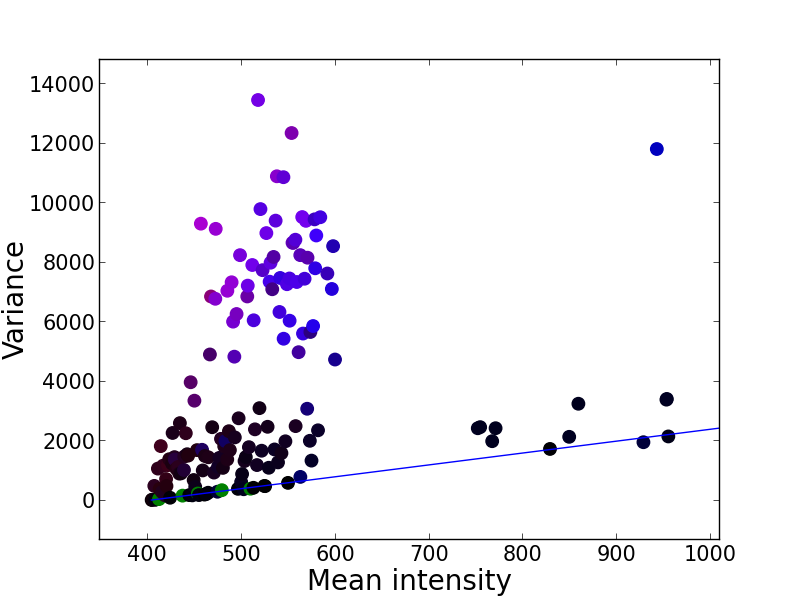
\includegraphics[width = .65\textwidth]{pictures/scatterplot_psfint_2000intmax_80_resx_150psfw_2.png}
\caption{Variance mean scatter plot of simulated data. The blue line indicates where pixels with constant mean would be displayed.}\label{simulatedScatter}
\end{figure}

\section{Variance vs Skellam}\label{skellambettervariance}
For the estimation of the camera gain and offset the method described in section \ref{estimationCameraGain} (Using variance-mean plot) is used. There are two different ways of estimating the variance of pixel intensities.\newline
The variance can be computed directly or the Skellam distribution as described in section \ref{skellamdist} can be used.\newline
The problem is to estimate the variance of the Poisson distribution of the pixels as good as possible, with as few samples as possible. The necessity to work well on as few frames as possible arises, as there can be data sets with only 200 or 300 frames or the user does not want to spend more time on the parameter estimation.\newline
To test which method for the variance estimation performs best, from a Poisson distribution with variance one, 200 samples are drawn, multiple times. Both methods were used to estimate the true variance. From all estimations the mean value of the estimated variance and the variance of the estimated variance were calculated. After that the procedure was repeated with increased true variance.\newline
Figure \ref{skellamvarmean} shows the results of the mean of the estimated variances, Figure \ref{skellamvarvar} shows the variance of the estimated variances, plotted over the true variance of the Poisson distribution.\newline
Figure \ref{skellamvarmean} shows, the mean estimates for the variance of a Poisson distribution with variances between zero and 40. The mean of all estimates from the Skellam approach is almost the same as the true variance (a straight line with slope one and zero intercept). The variance approach underestimates the true variance. Figure \ref{skellamvarvar} shows the variances of the estimates for both approaches. The variance approach has a lower variance than the Skellam approach.\newline
Only one estimate is calculated in practice, therefore the variance approach is taken, as the variance of the estimated values is lower.

%\begin{figure}
%\begin{minipage}{0.48\textwidth}
%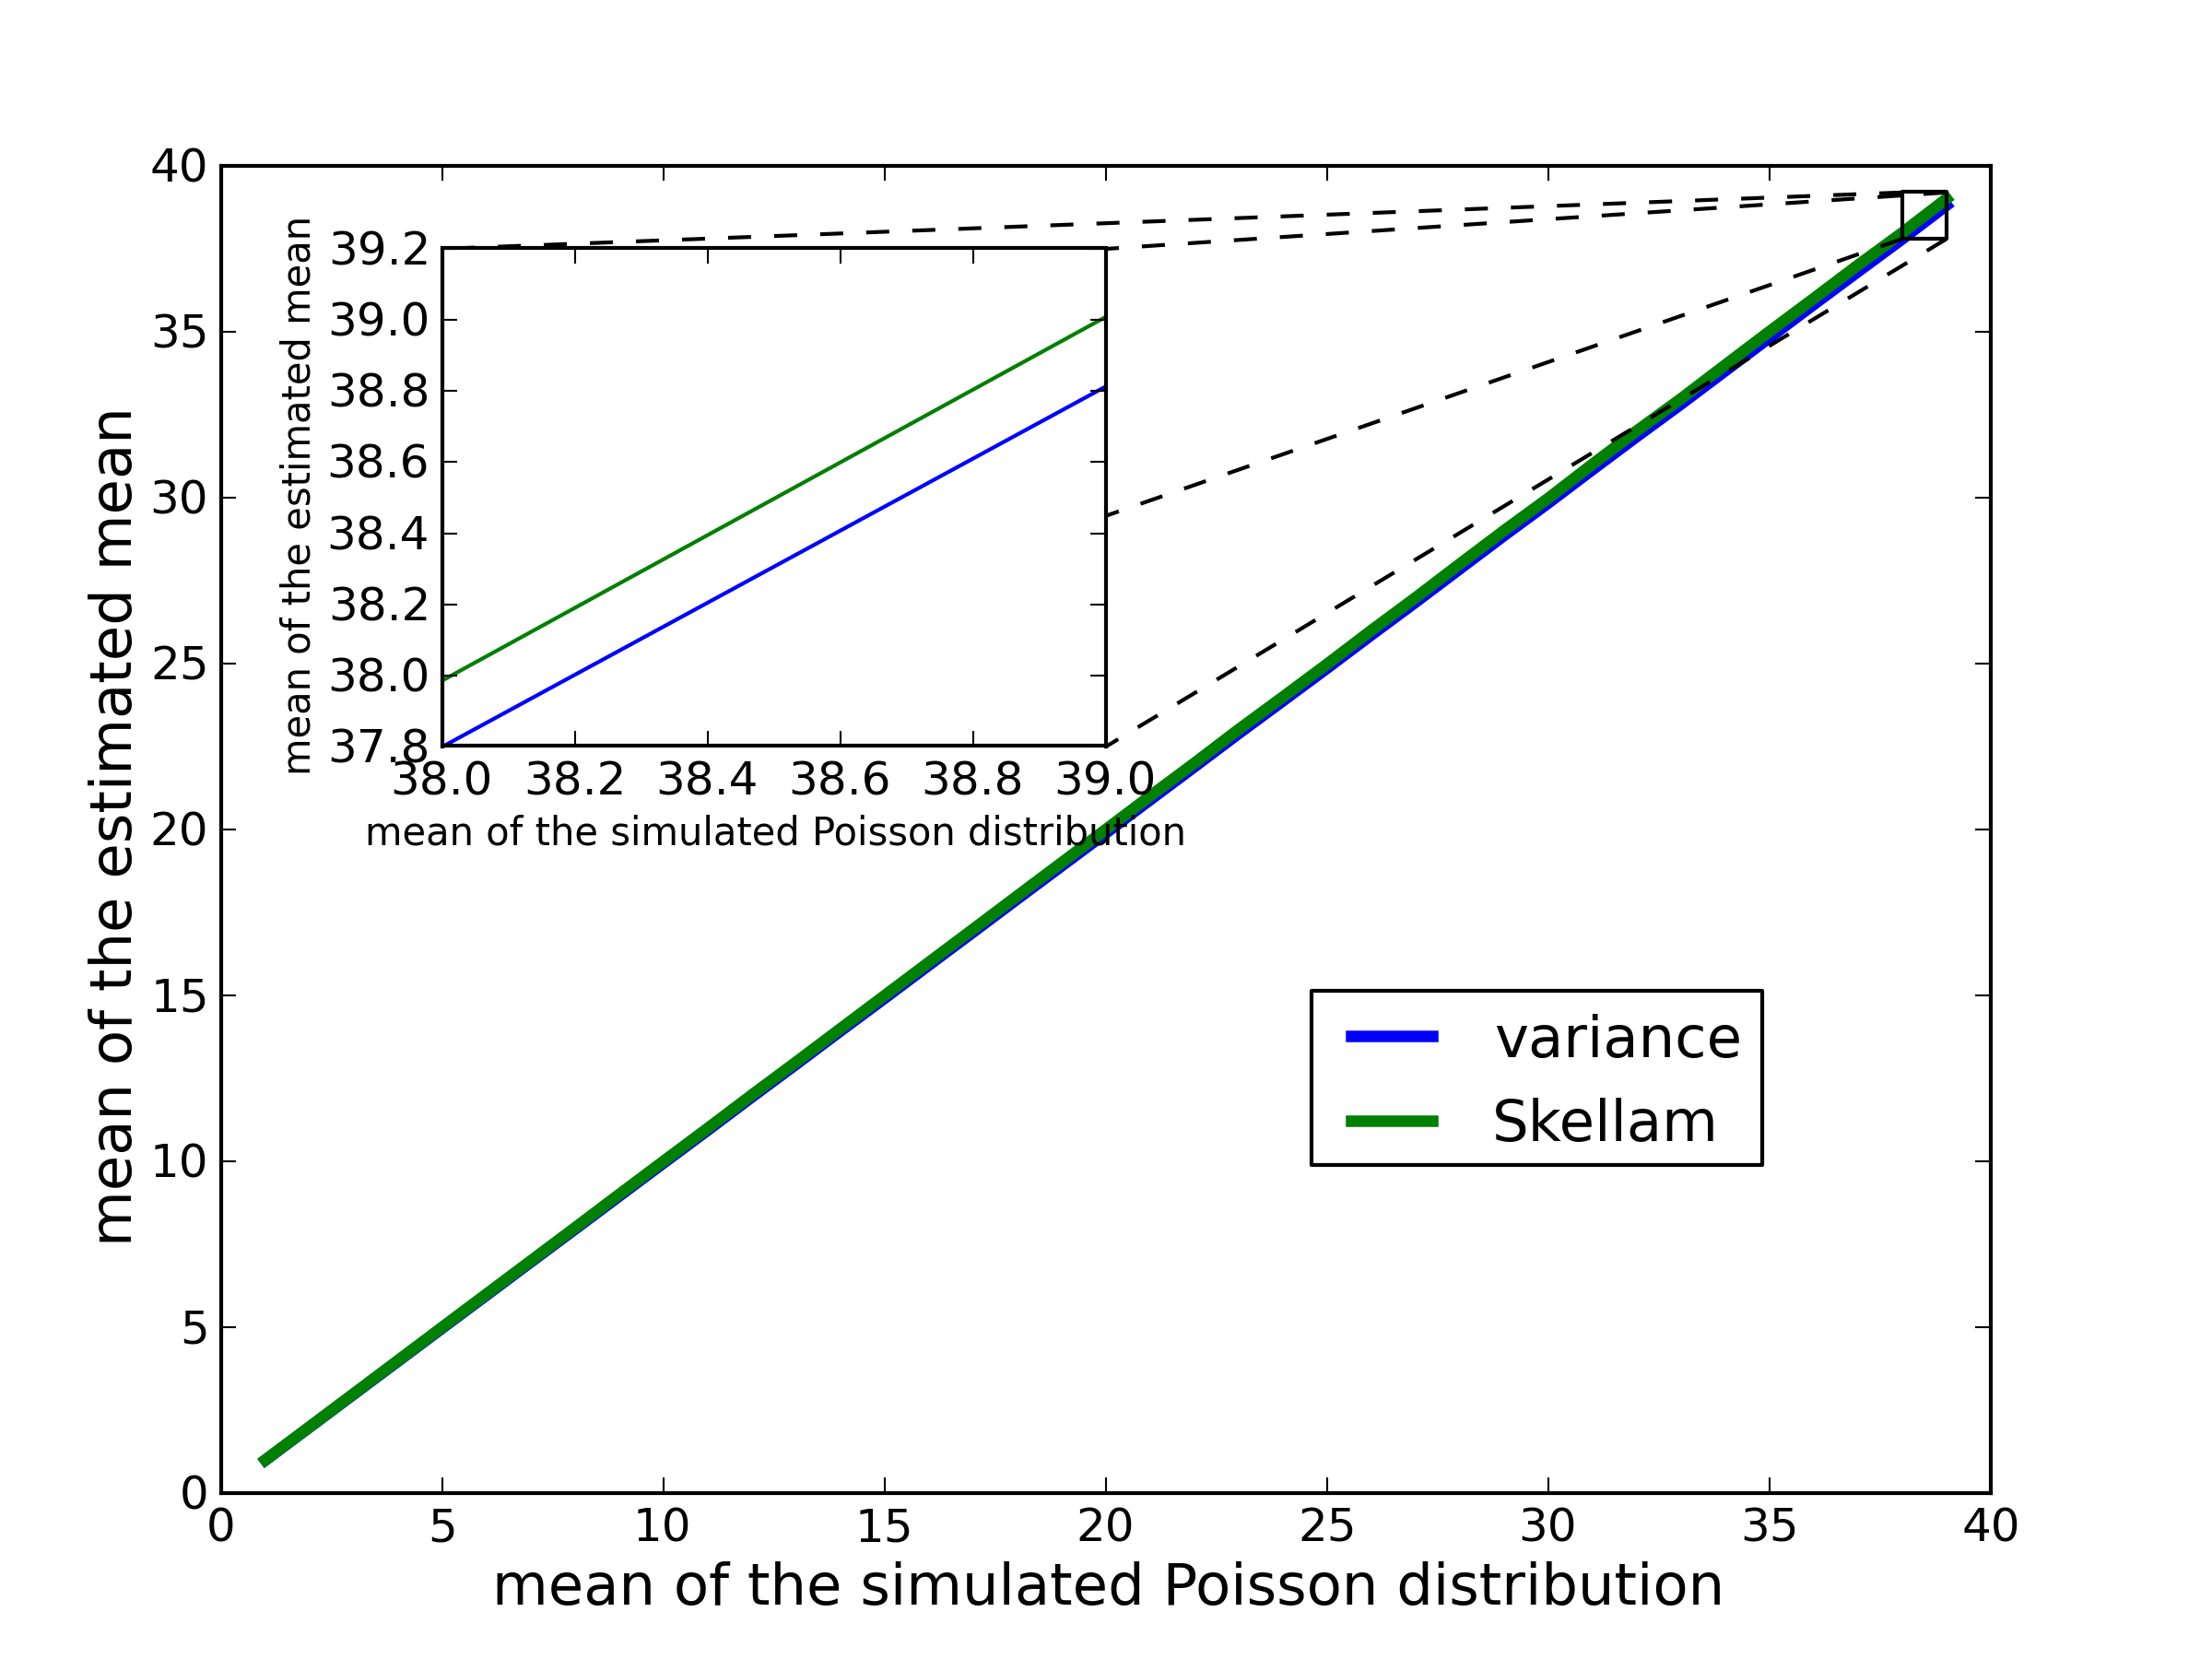
\includegraphics[width = \textwidth]{pictures/SkellamVarMean.png}
%\caption{Mean of the estimated variances.}\label{skellamvarmean}
%\end{minipage} \hfill
%\begin{minipage}{0.48\textwidth}
%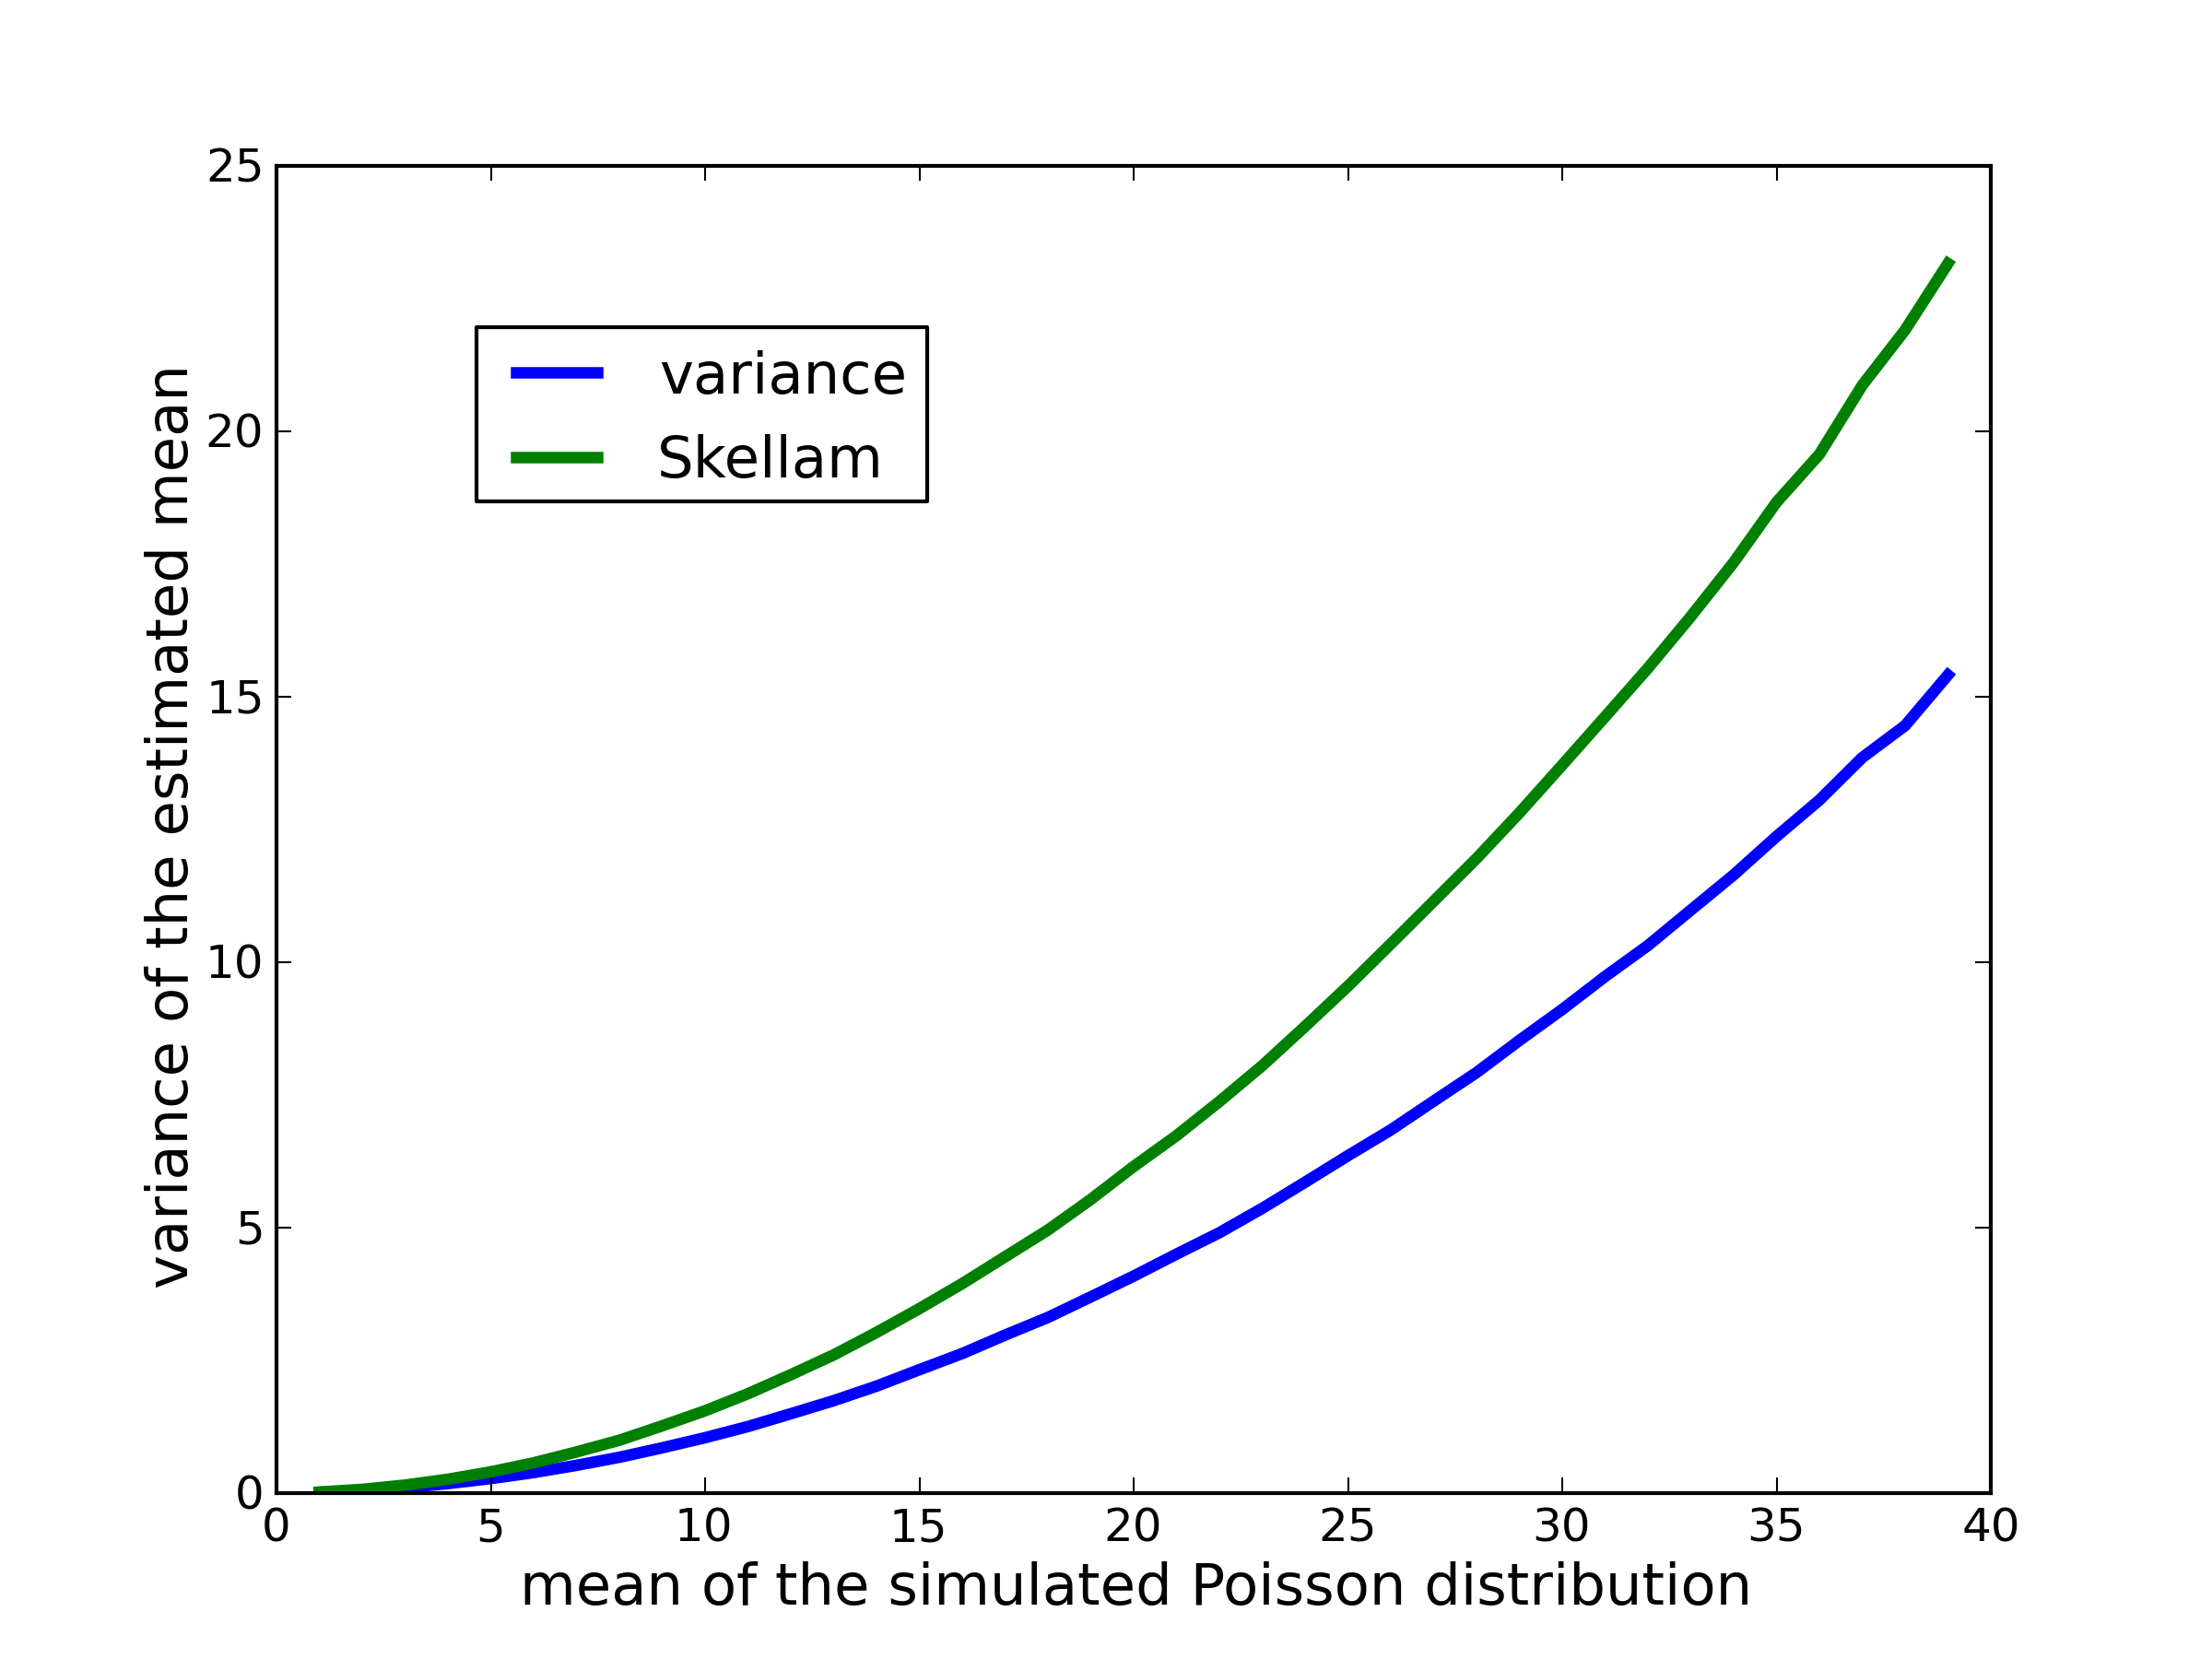
\includegraphics[width = \textwidth]{pictures/SkellamVarVar.png}
%\caption{Variance of the estimated variances.}\label{skellamvarvar}
%\end{minipage}
%\end{figure}

\begin{figure}
\centering
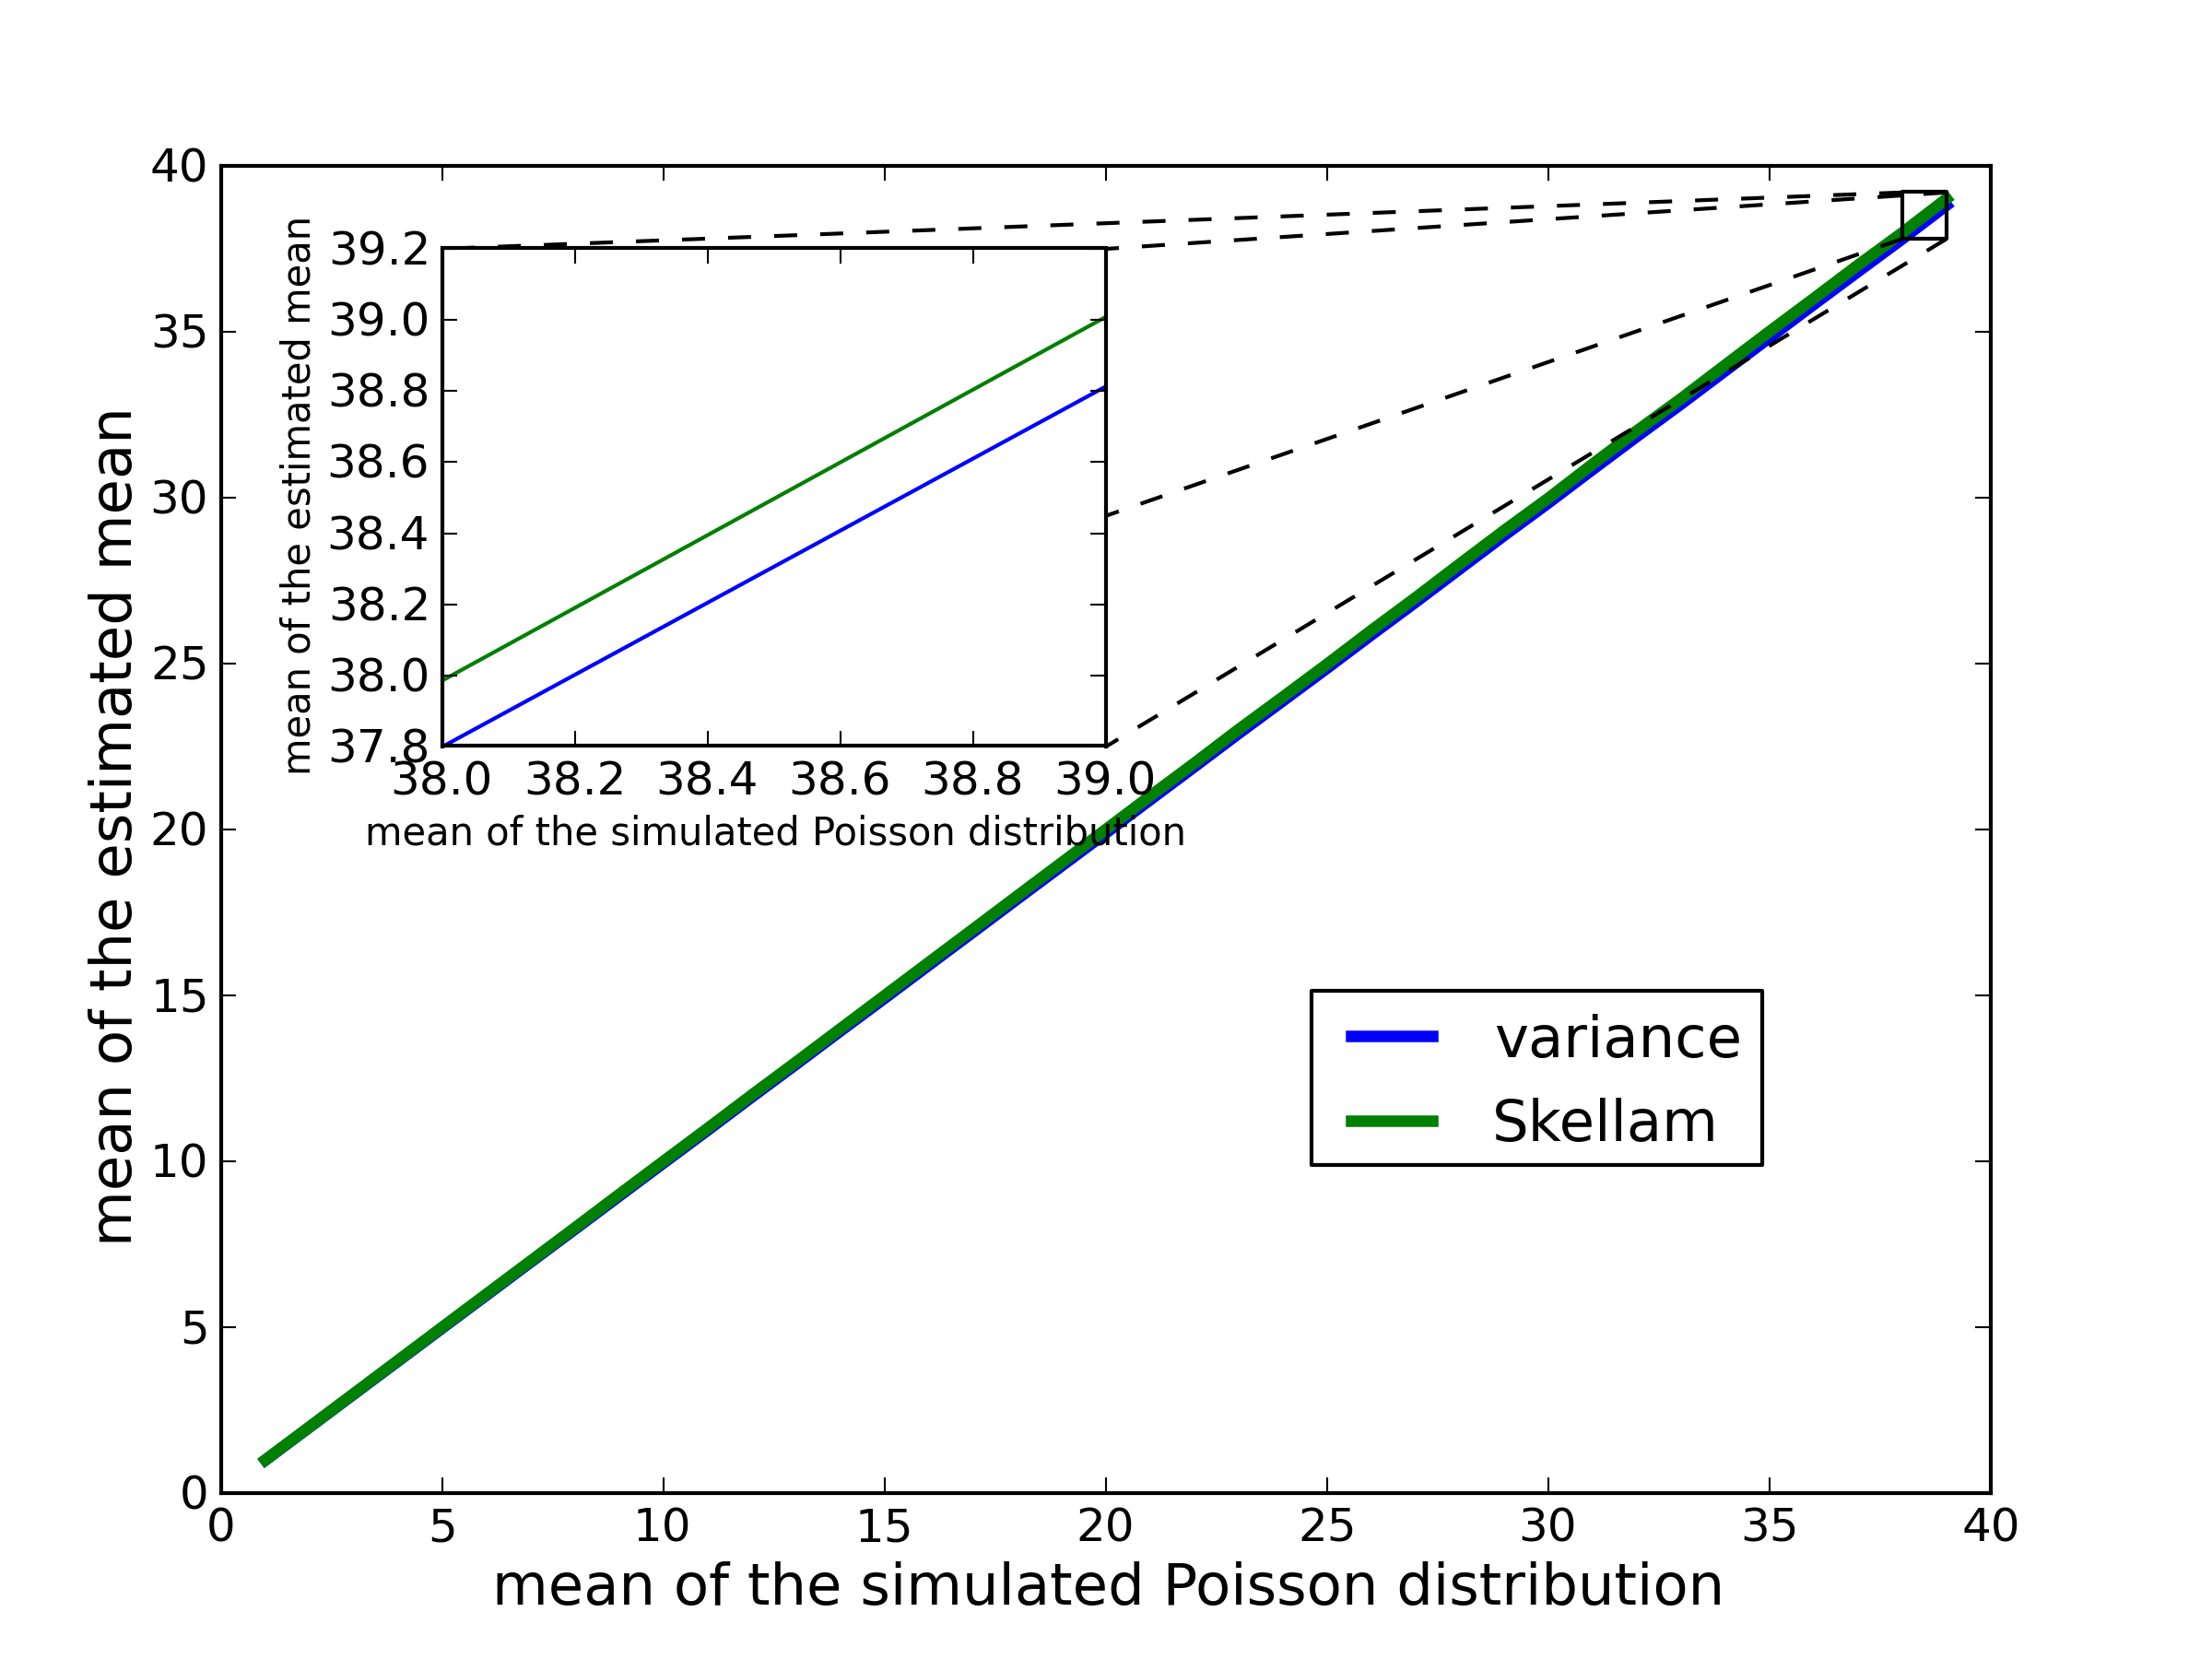
\includegraphics[width = .7\textwidth]{pictures/SkellamVarMean.png}
\caption{Mean of the estimated variances.}\label{skellamvarmean}
\end{figure}

\begin{figure}
\centering
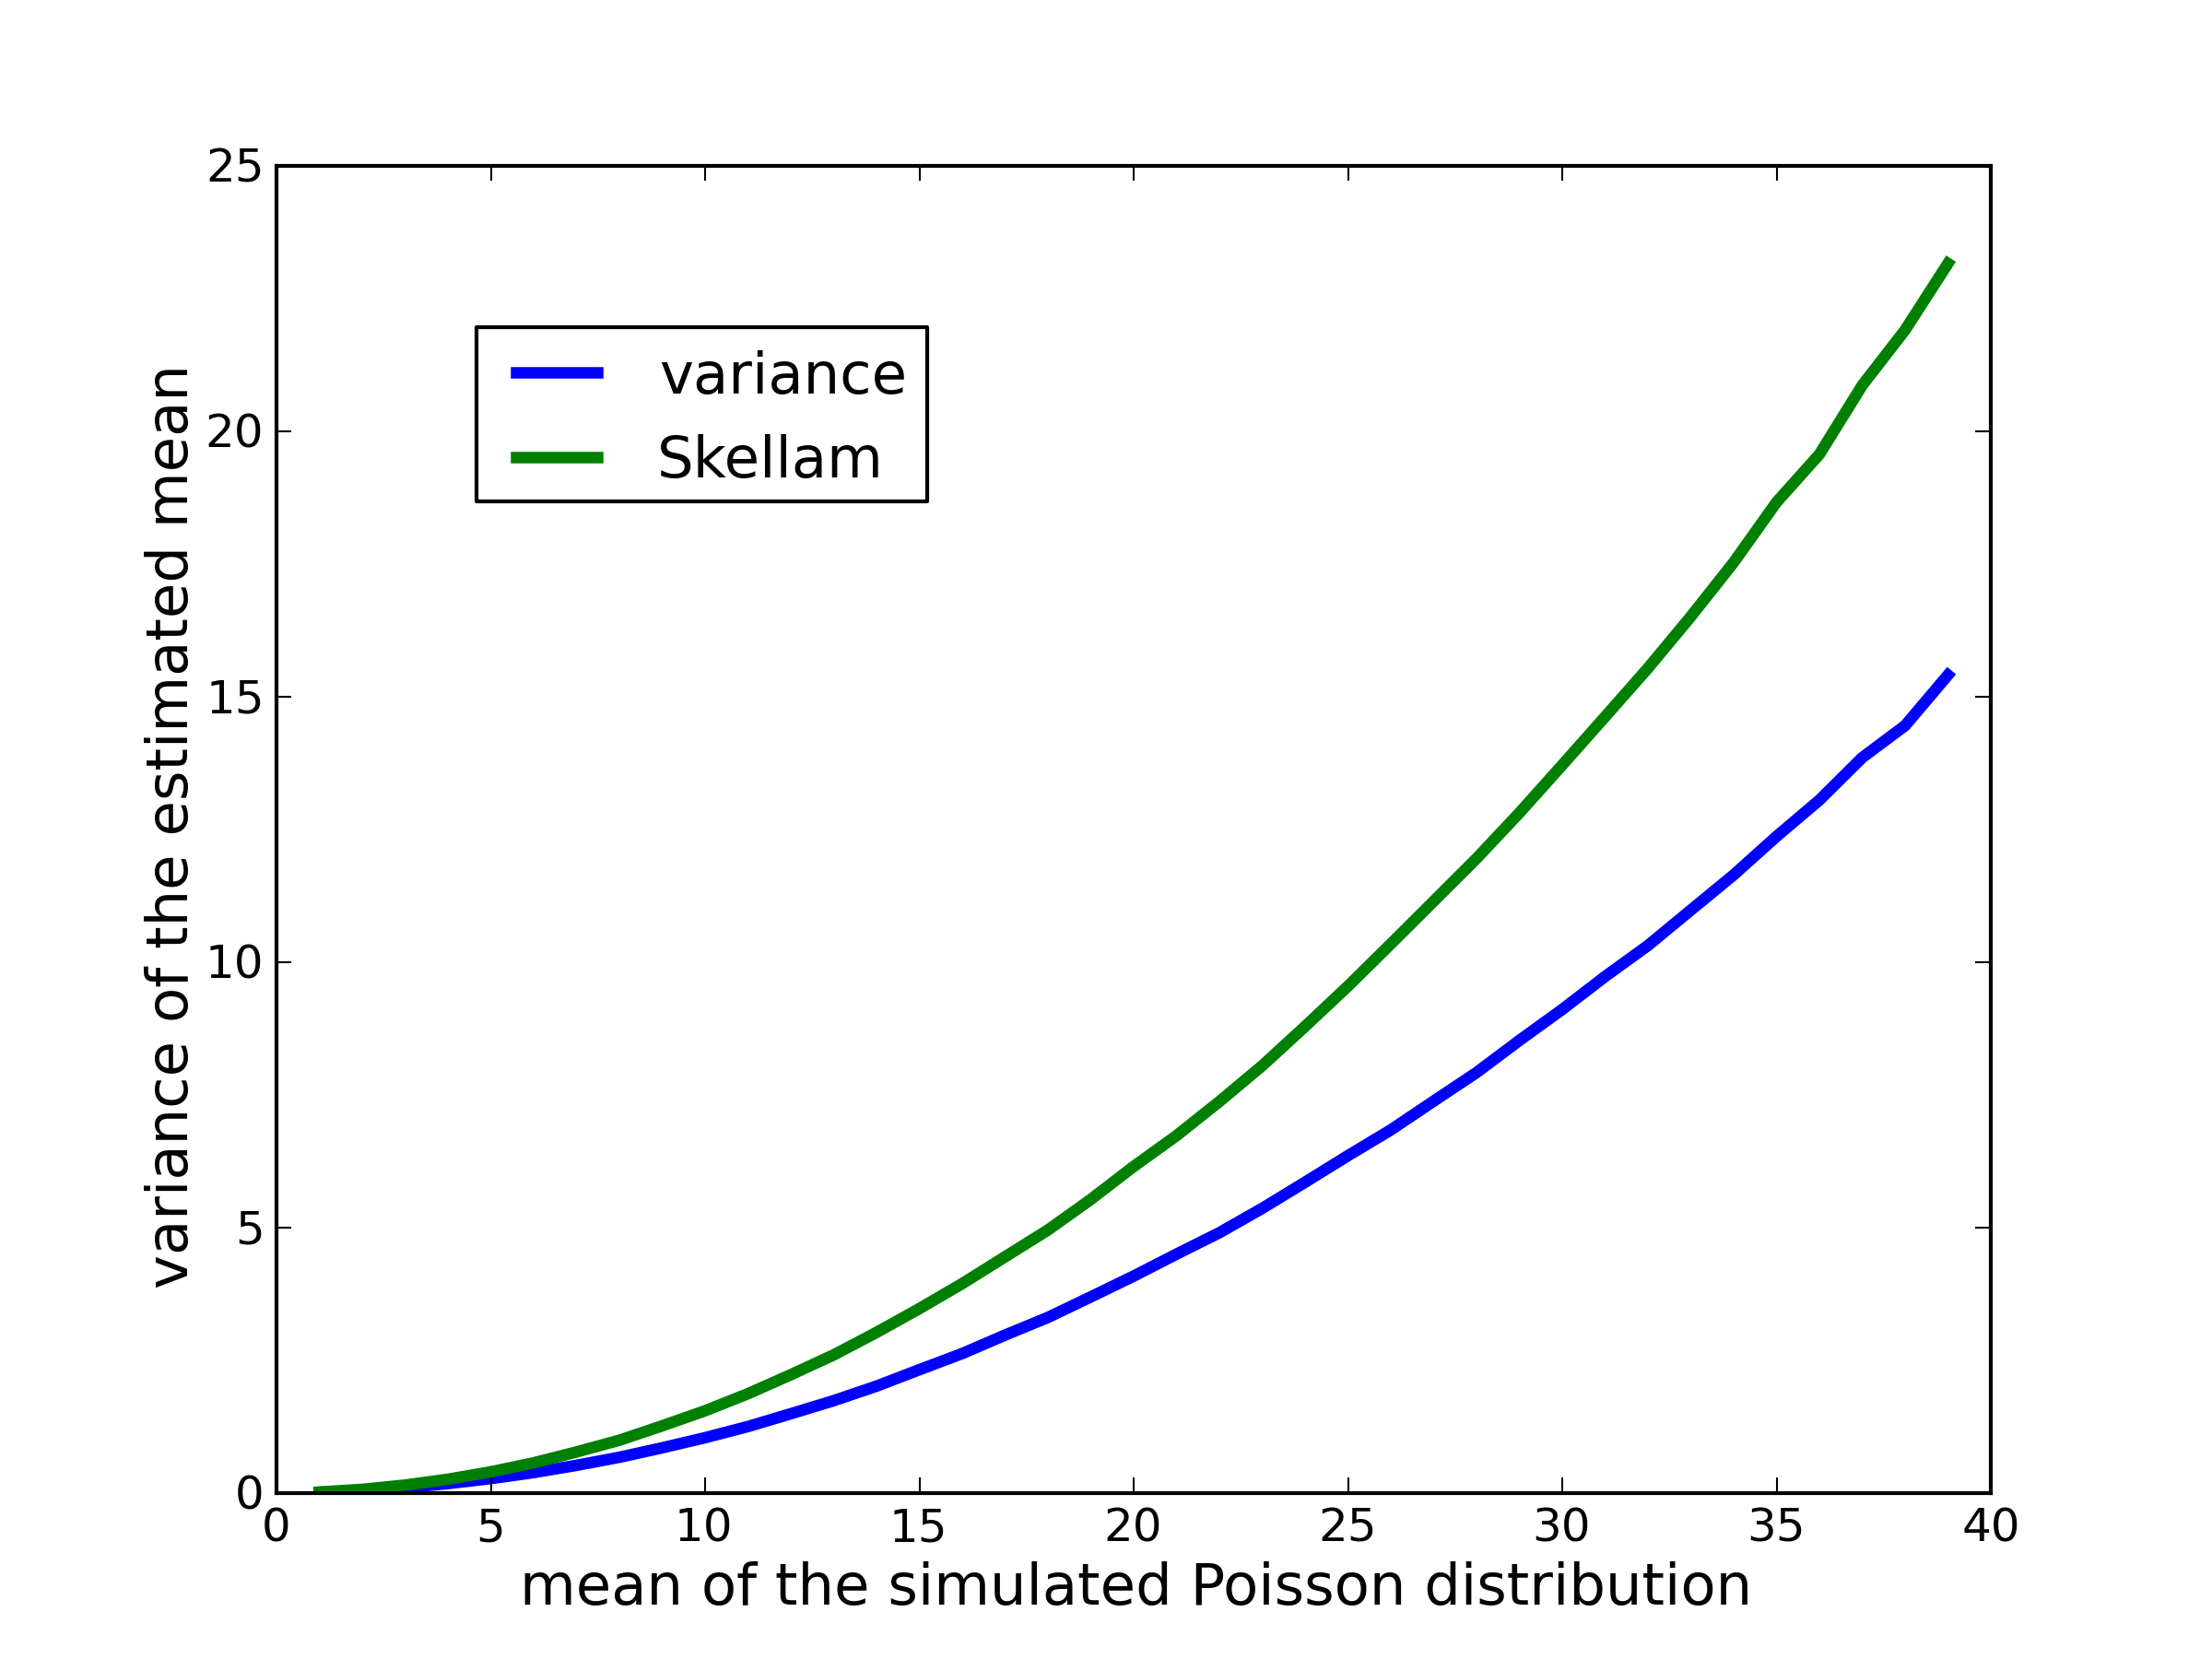
\includegraphics[width = .7\textwidth]{pictures/SkellamVarVar.png}
\caption{Variance of the estimated variances.}\label{skellamvarvar}
\end{figure}


\section{Best line fit method}
To get the correct gain and offset based on the mean intensities and the corresponding variances of the pixels intensities, a robust fitting method is needed. This is because of the many outlier as seen in Figure \ref{simulatedScatter}. In this section six different methods will be described and their performances compared.
\subsection{Different methods}
\subsubsection*{Based on minimum covariance determinant (Fit1)}
The base of this fitting approach is to find a compact subset of points that represents the inliers. To do so a R function based on the algorithm of \cite{ilia1} is used. For this algorithm many initial subsets of  the data are drawn. For each subset of points the minimal covariance determinant is calculated. The subset with the smallest covariance determinant is taken. Weighted linear regression is performed on the selected subset of points. Therefore the $x$ range is split into several bins. For each bin the variance of the points is calculated and its inverse is used as weights for linear regression.\newline
This fitting algorithm was developed and implemented in cooperation with Ilia Kats.
\subsubsection*{Use only lowest variances, weighted (Fit2)}
Thousand iterations are used. For each iteration half of the preselected points is chosen randomly. 
The mean values are split into bins of equal width. For each bin the variance of the variances is calculated. Within each bin the point with the lowest variance is found. Linear regression is performed on all these lowest points with the inverse variance of variances of each bin as weights. The fit with the least error is kept.
\subsubsection*{Linear fit of a random number of points (Fit3)}
The difference to the approach described in Fit2 is that the lowest points within each bin are found based on all data, then a linear fit is performed on a subset of varying size several times.
\subsubsection*{RANSAC (Fit4) and weighted RANSAC (Fit5)}\label{ransacdescr}
A standard RANSAC (random sample consensus) algorithm is used. Its pseudo code is shown below:
\begin{verbatim}
input:
    data - set of mean intensities and variances
    model - straight line 
    k - number iterations
    t - threshold for determining if a point fits the model
    d - number of close points that must be found at least not to 
        discard the found model instantly
output:
    slope m and intercept c of the straight line

iteration = 0
best_m = 0
best_c = 0
best_error = inf
while iterations < k
    initial_guess_set = 2 random points from data
    m,c = fit_line(initial_guess_set)
    for every point in data
        if |y_point - m*x_point+c| < t
            add point to consensus_set
    m,c,current_error = fit_line(consensus_set)
    if len(consensus_set)>d and current_error < best_error
        best_error = current_error
        best_m = m
        best_c = c

return best_m, best_c
\end{verbatim}
For the weighted RANSAC instead of a linear fit, a weighted line fit is done. The weights are determined as for the other weighted fitting methods.
\subsubsection*{Simple fit (Fit6)}
For this very simple approach, a certain number of points is chosen randomly from all points. A straight line is fitted and the mean square error for the current set of points is computed. This is done several times. The best fit with the lowest mean square error is taken as final result.

\subsection{Discussion} 
The goal is to find a robust fitting method. Figures \ref{lineplot1} and \ref{lineplot2} show scatter plots of the means and variances of the preselected points and the results of the fits.
It is difficult to determine the best fit by looking at the results, since the correct line is not clearly visible.
The calibration measurement yields a gain factor of 3.9 and a offset off 380. Table \ref{tablefits} shows the fit results for offset and gain. The results from both RANSAC methods (Fit 4/5) are closer to the results from the calibration measurement than any other fitting methode. This table also illustrates why for the offset the minimal value is used instead of the estimated value, there is much variation in the intersection with the $x$-axis.\newline
For the parameter estimation the weighted RANSAC method is used.\newline
It is important to mention that the weighting that is used weights points from smaller intensities more than for higher intensities. The reason is that only the variance is considered which increases with increasing mean intensities. This is done on purpose. The lower intensities, originated by the background pixels show the desired line behaviour most clearly. Another advantage is that this approach is not absolutely dependent on beads, which give points in the scatter plot for high means. 

\begin{minipage}{\textwidth}
\begin{footnotesize}
\begin{center}
%\caption{Results for the main submission (with postprocessing)}
\captionof{table}{Fitting results for gain and offset for various data sets from our collaborators from Bioquant.}\label{tablefits}%
\begin{tabular}{l||c|c||c|c||c|c||c|c||c|c||c|c||}
Data set&\multicolumn{2}{c||}{Fit 1}&\multicolumn{2}{c||}{Fit 2}&\multicolumn{2}{c||}{Fit 3}&\multicolumn{2}{c||}{Fit 4}&\multicolumn{2}{c||}{Fit 5}&\multicolumn{2}{c||}{Fit 6}\\
&$g$&$o$&$g$&$o$&$g$&$o$&$g$&$o$&$g$&$o$&$g$&$o$\\\hline
110215\_HeLa1\_Er647&21.4&435&16.6&430&20.0&474&2.37&282&4.17&350&8.37&402\\\hline
110302\_ER-Alexa647&12.3&458&19.1&432&11.3&479&4.42&358&4.42&358&8.00&410\\\hline
110302\_HeLa1\_ER647&7.56&437&6.45&452&6.68&474&3.22&228&2.69&156&4.21&269\\\hline
Pos2\_2\_green&12.6&484&7.05&452&7.12&483&3.13&308&3.44&329&5.76&407\\\hline
Pos2\_2\_red&6.67&378&7.26&443&7.78&474&3.82&374&4.31&380&6.18&396\\\hline
Pos11\_2\_green&12.9&442&8.17&395&9.15&474&4.51&376&4.59&378&5.83&390\\\hline
Pos11\_2\_red&11.0&390&20.3&839&10.6&443&3.78&359&3.84&361&9.89&416\\\hline
Tetra1\_high\_568&5.33&387&4.74&394&3.97&387&4.11&379&4.12&380&4.68&382
\end{tabular} 

\end{center}
\end{footnotesize}
\end{minipage} 
 
\begin{figure}
\subfloat[110215\_HeLa1\_Er647]{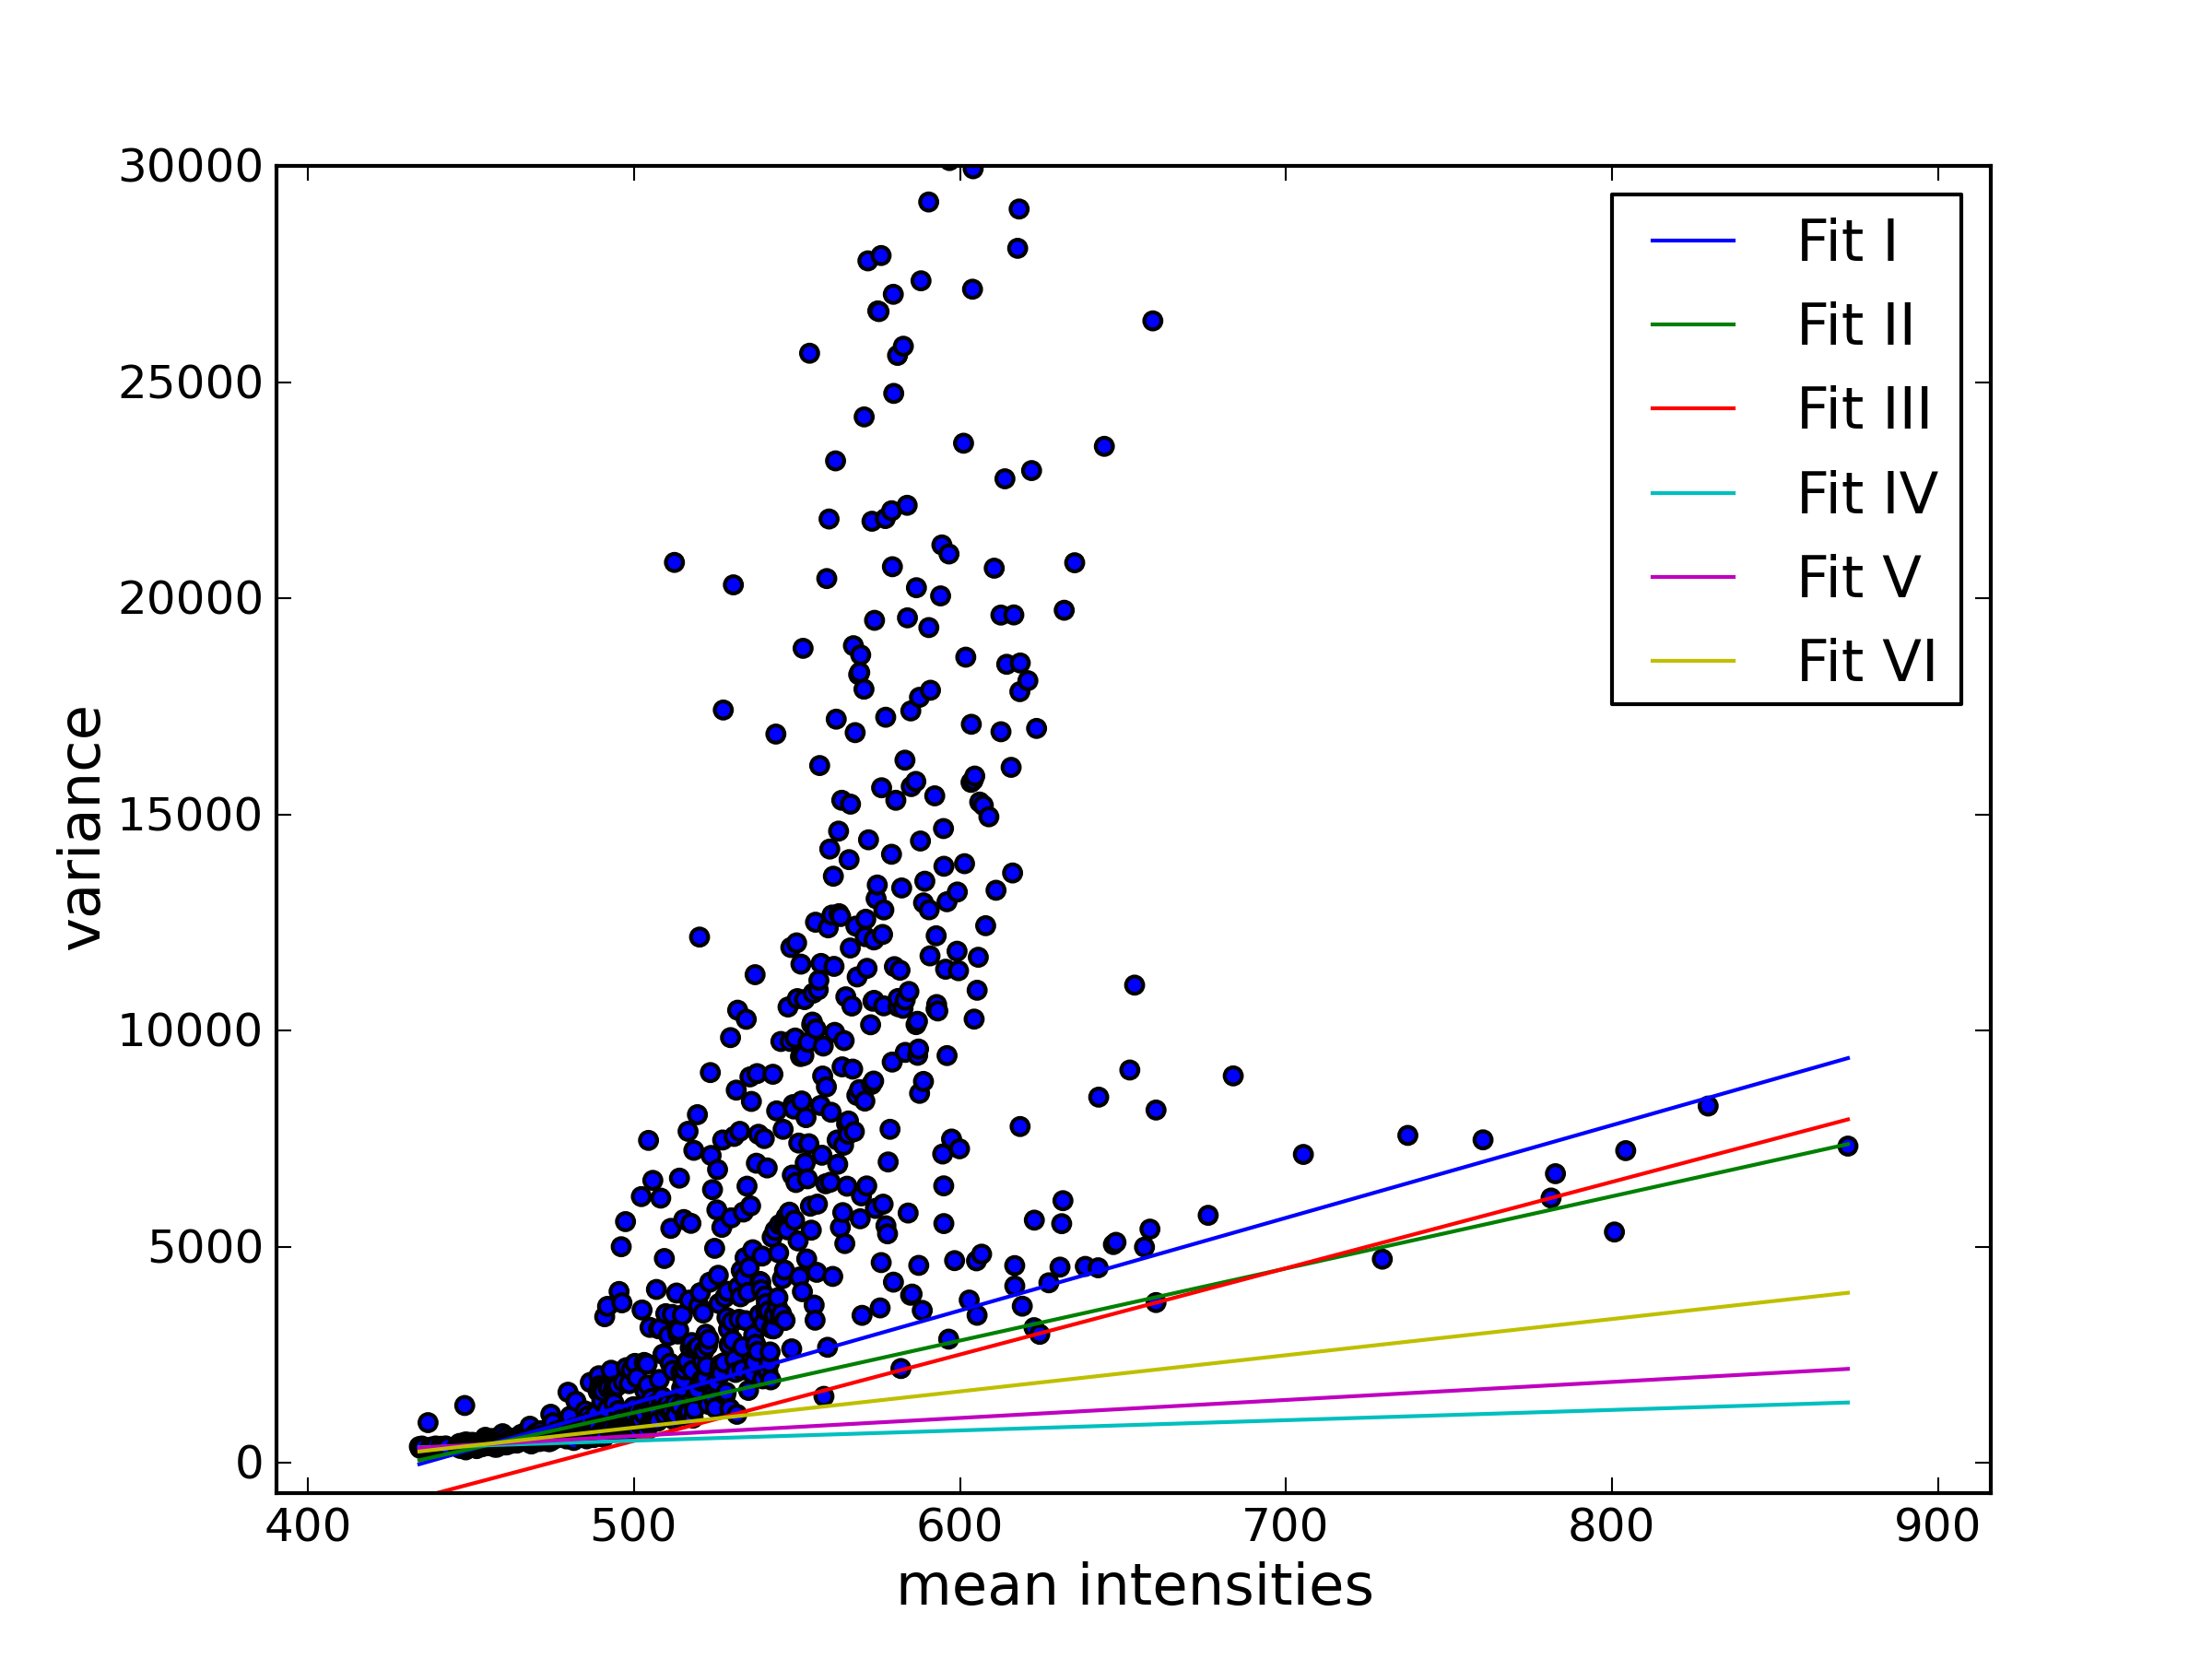
\includegraphics[width =0.48\textwidth]{pictures/geradenplots/110215hela.png}}\hfill
\subfloat[110302\_ER-Alexa647]{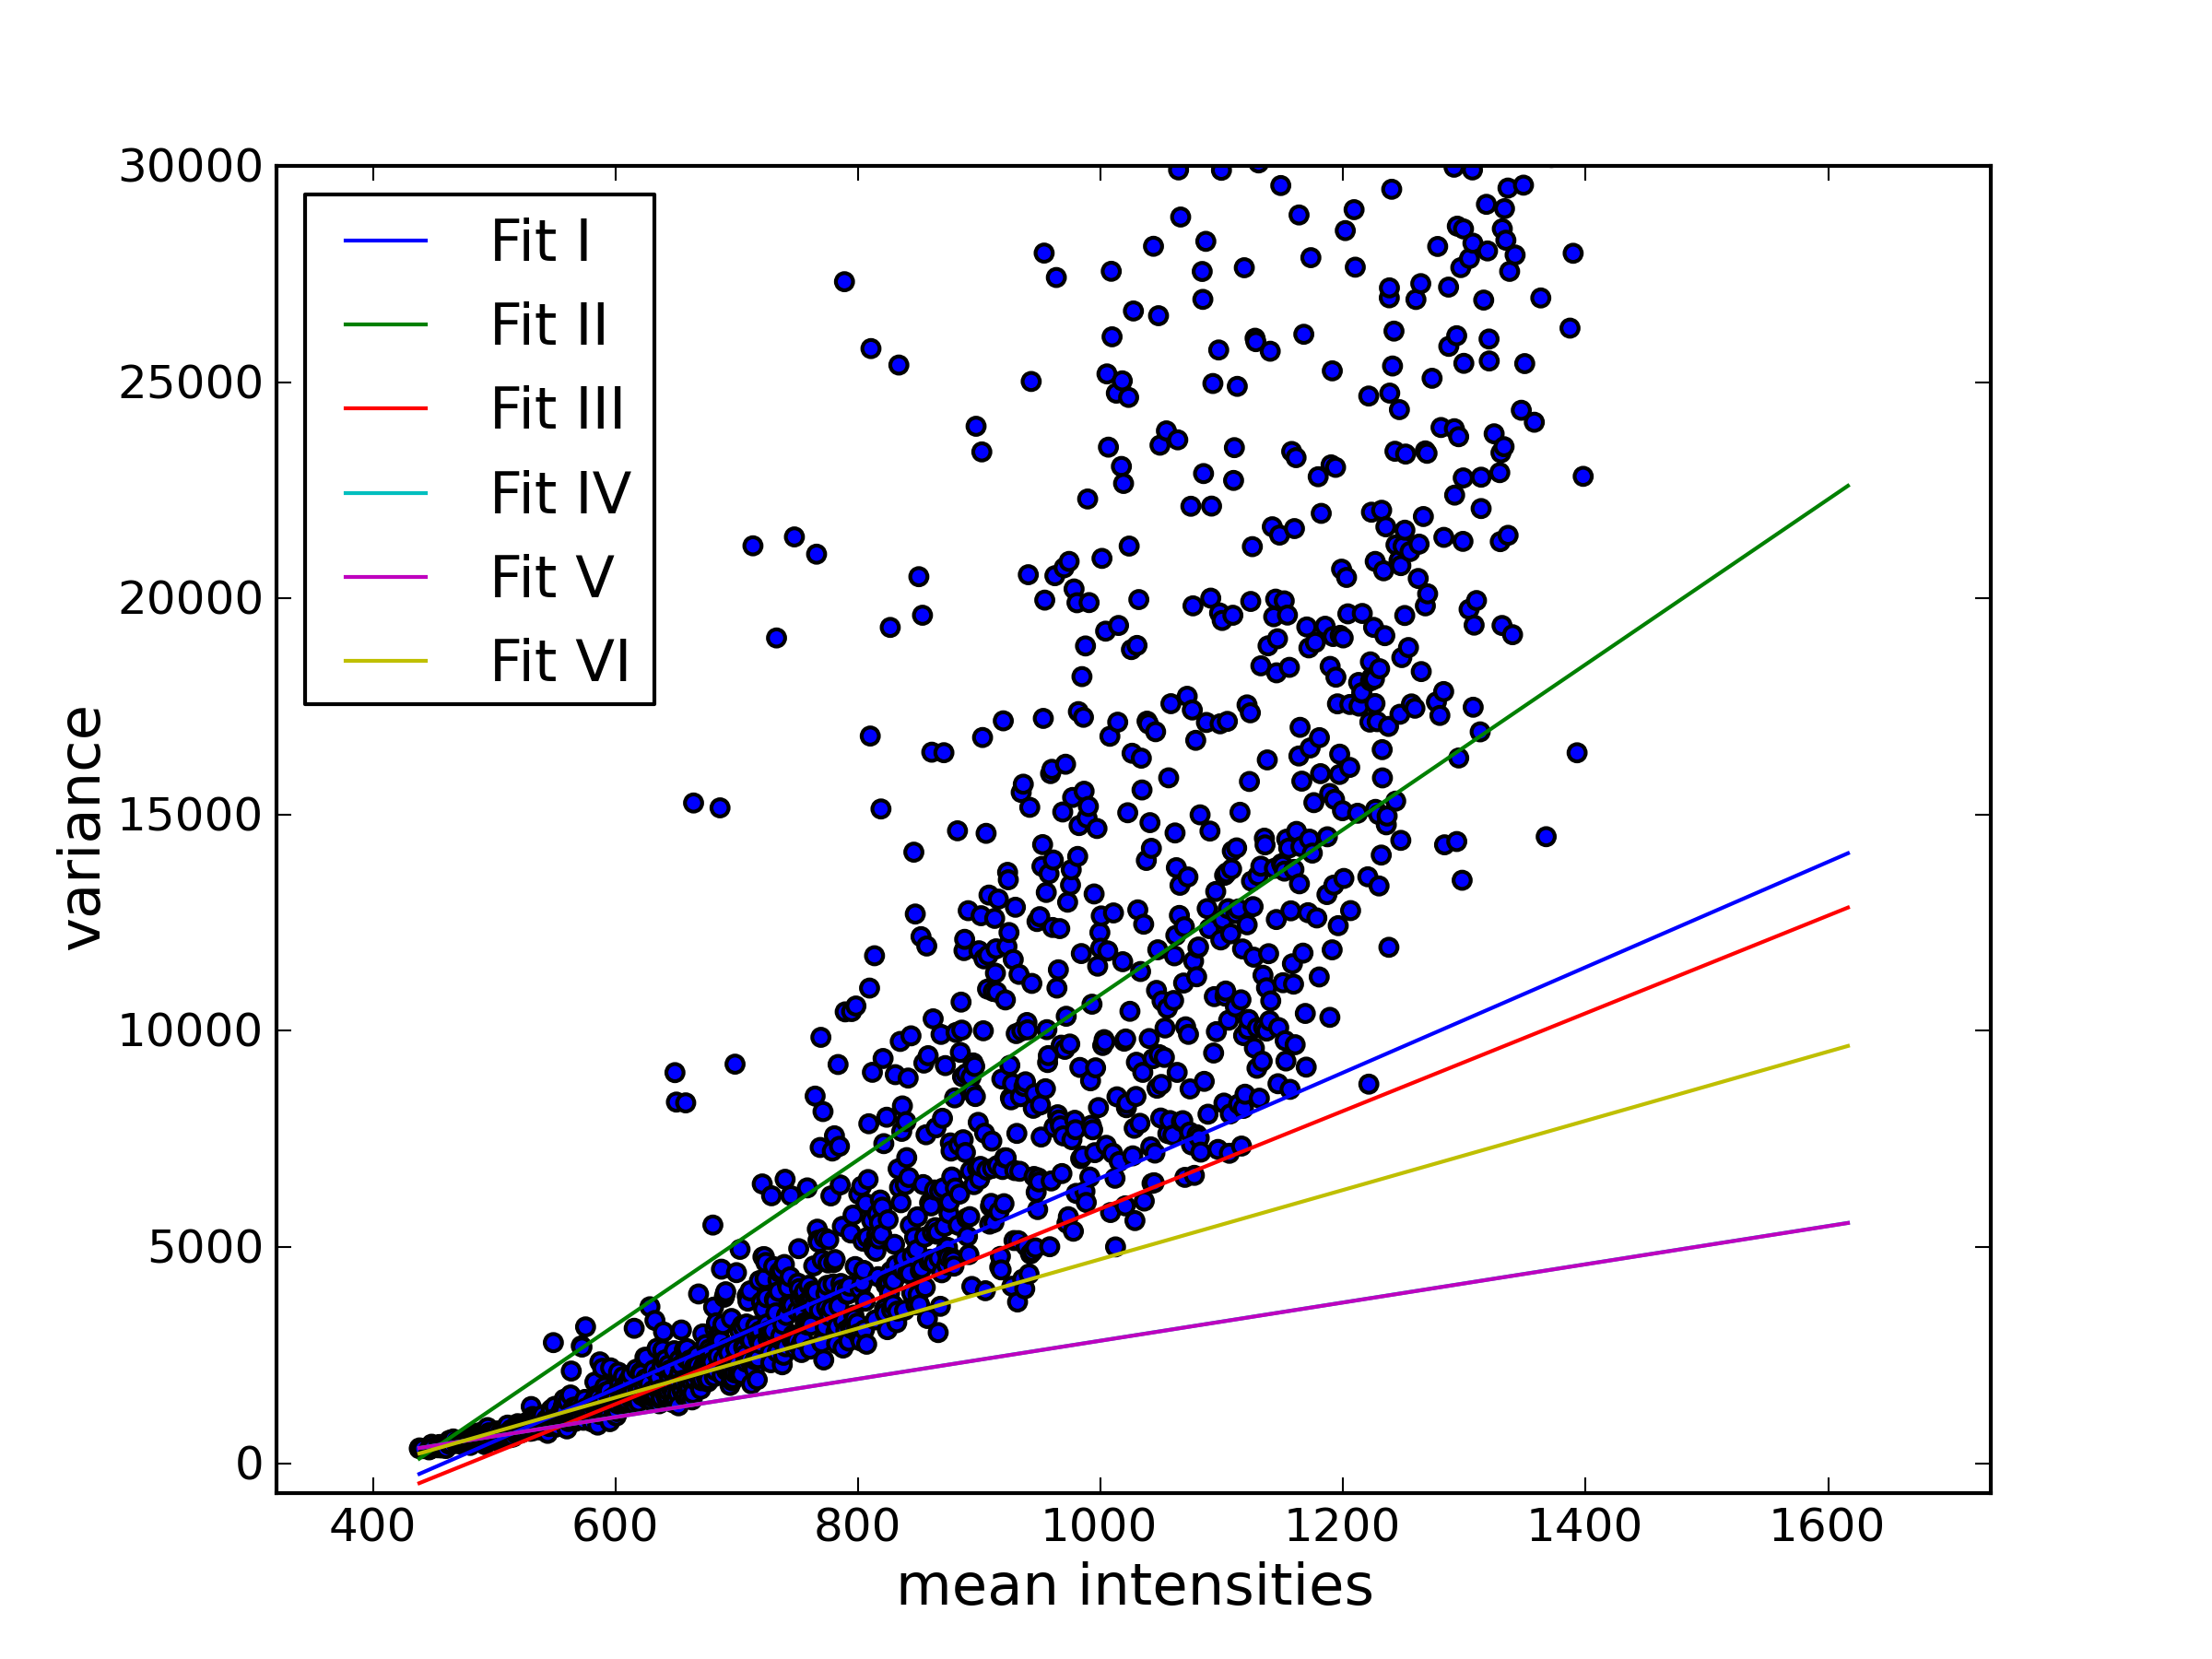
\includegraphics[width =0.48\textwidth]{pictures/geradenplots/110302alexa647.png}}\\
\subfloat[110302\_HeLa1\_ER647]{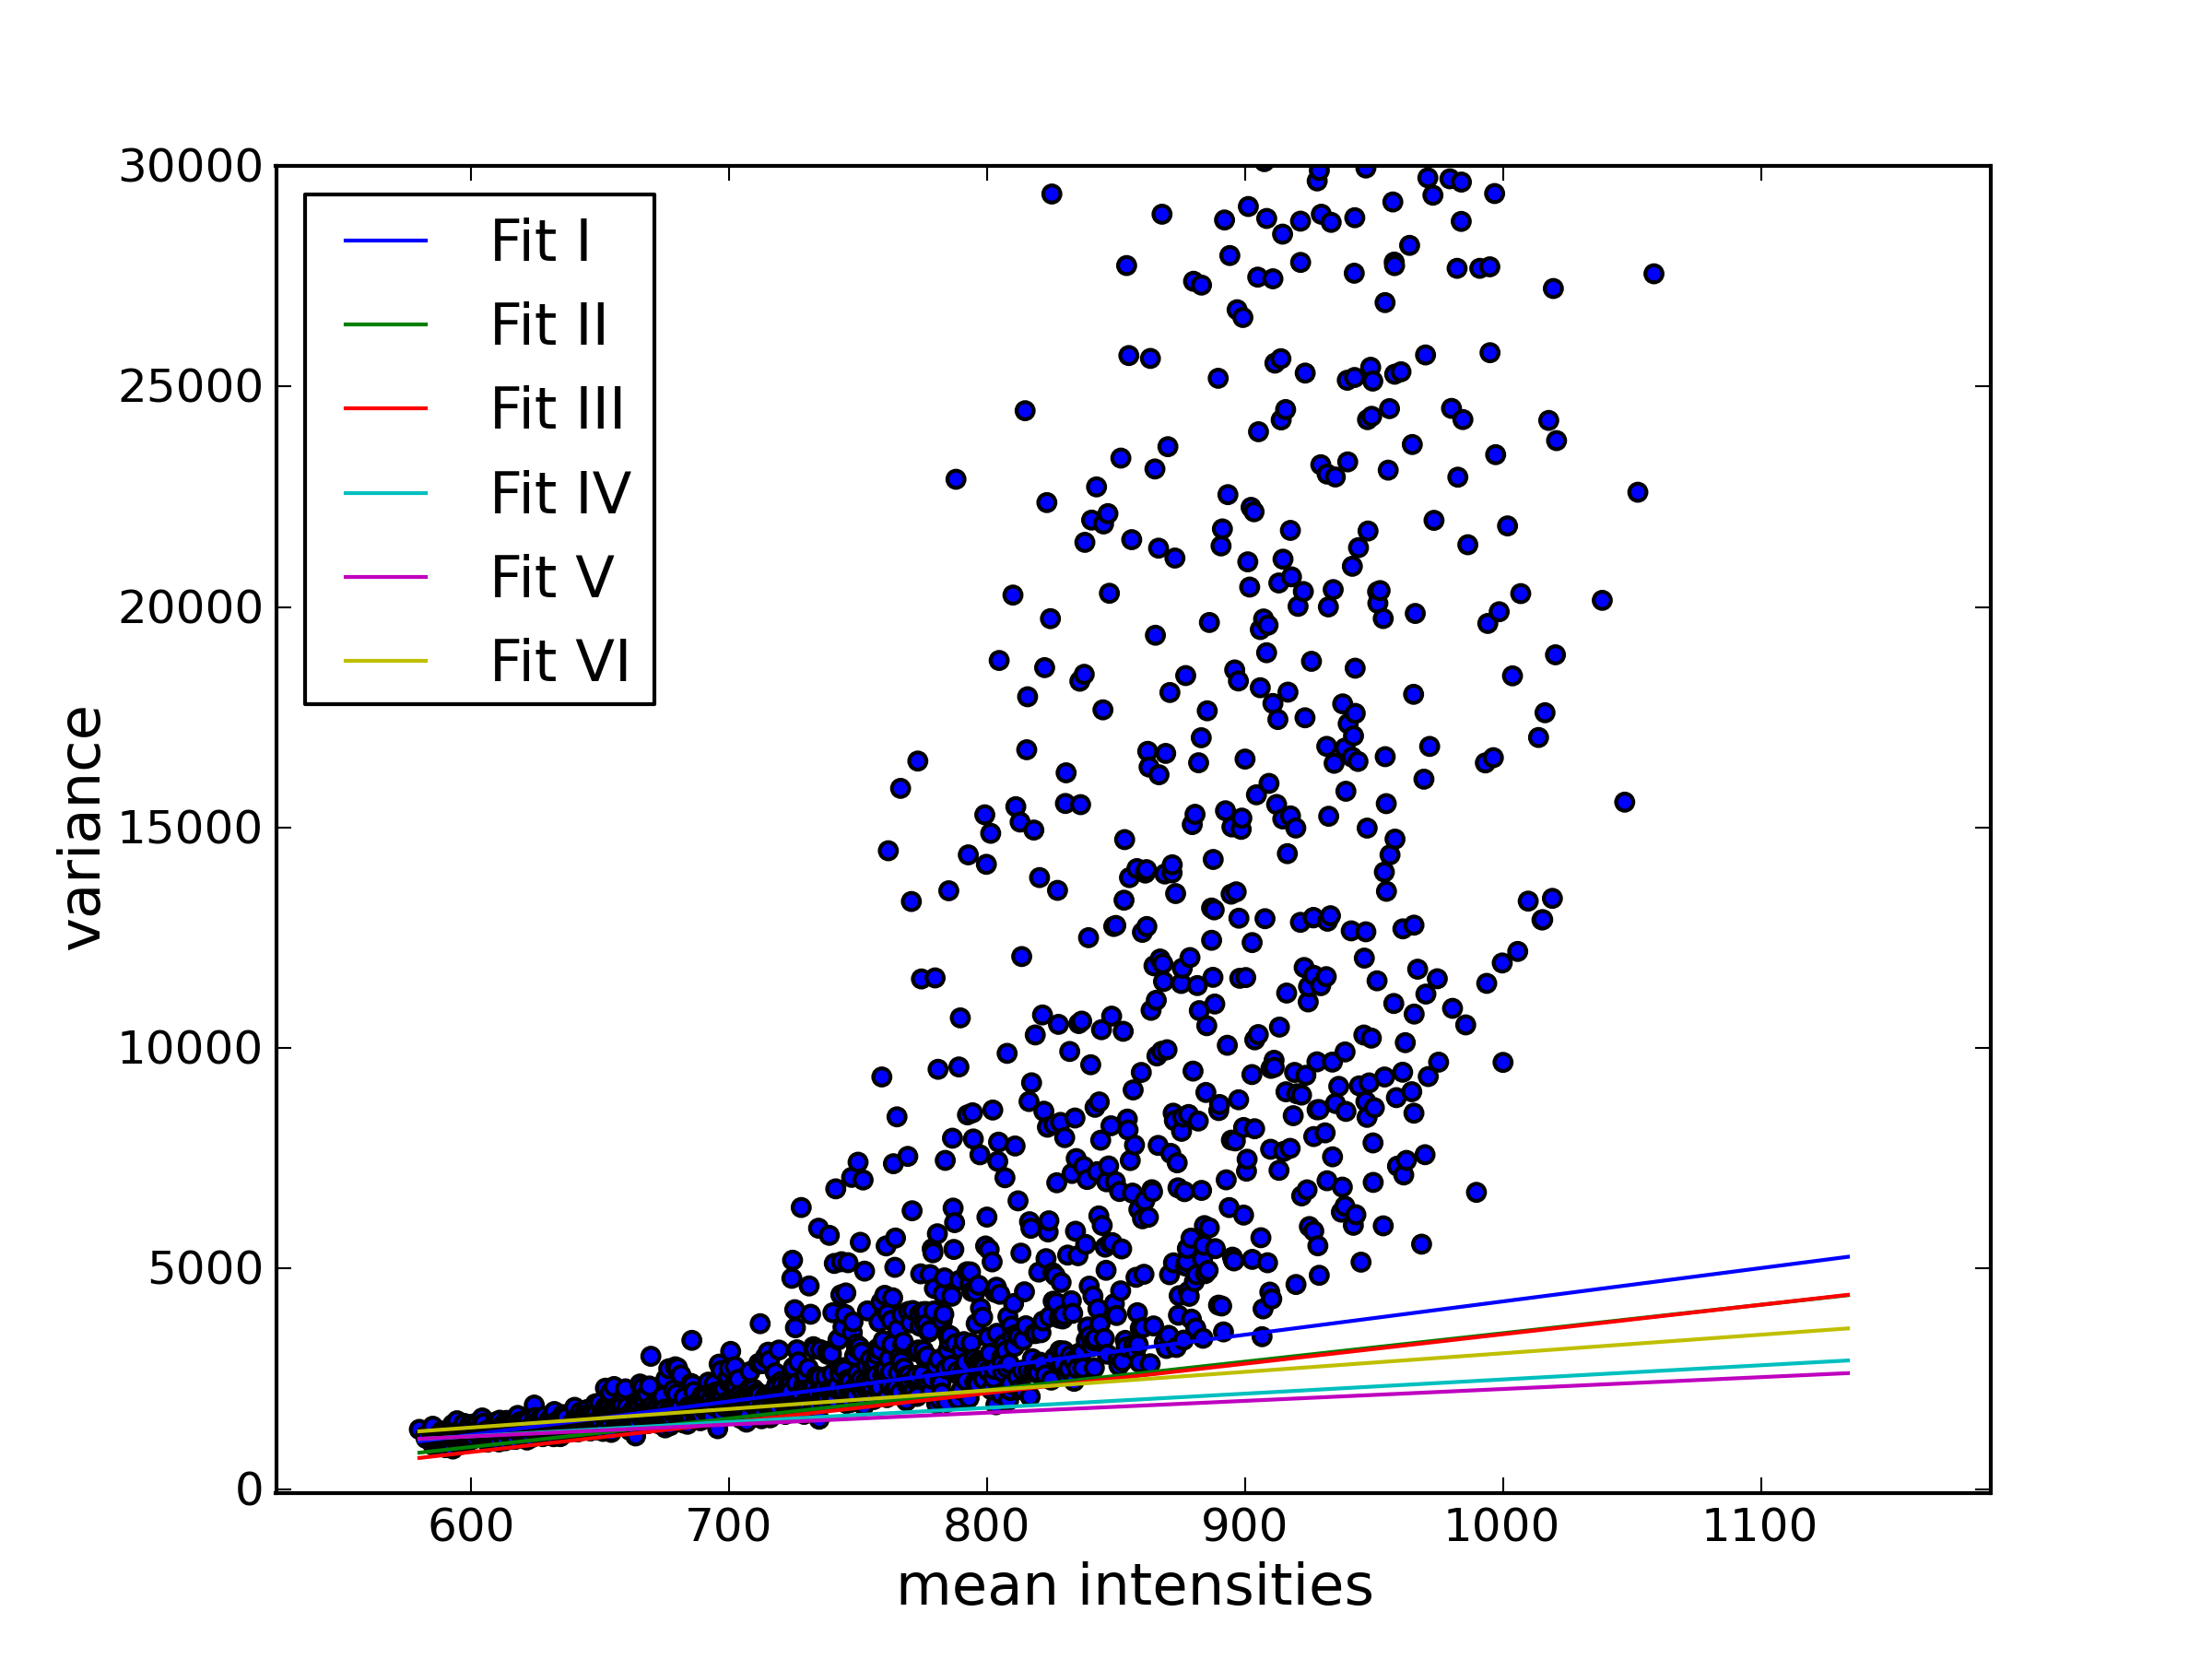
\includegraphics[width =0.48\textwidth]{pictures/geradenplots/110302hela647.png}}\hfill
\subfloat[Pos2\_2\_green]{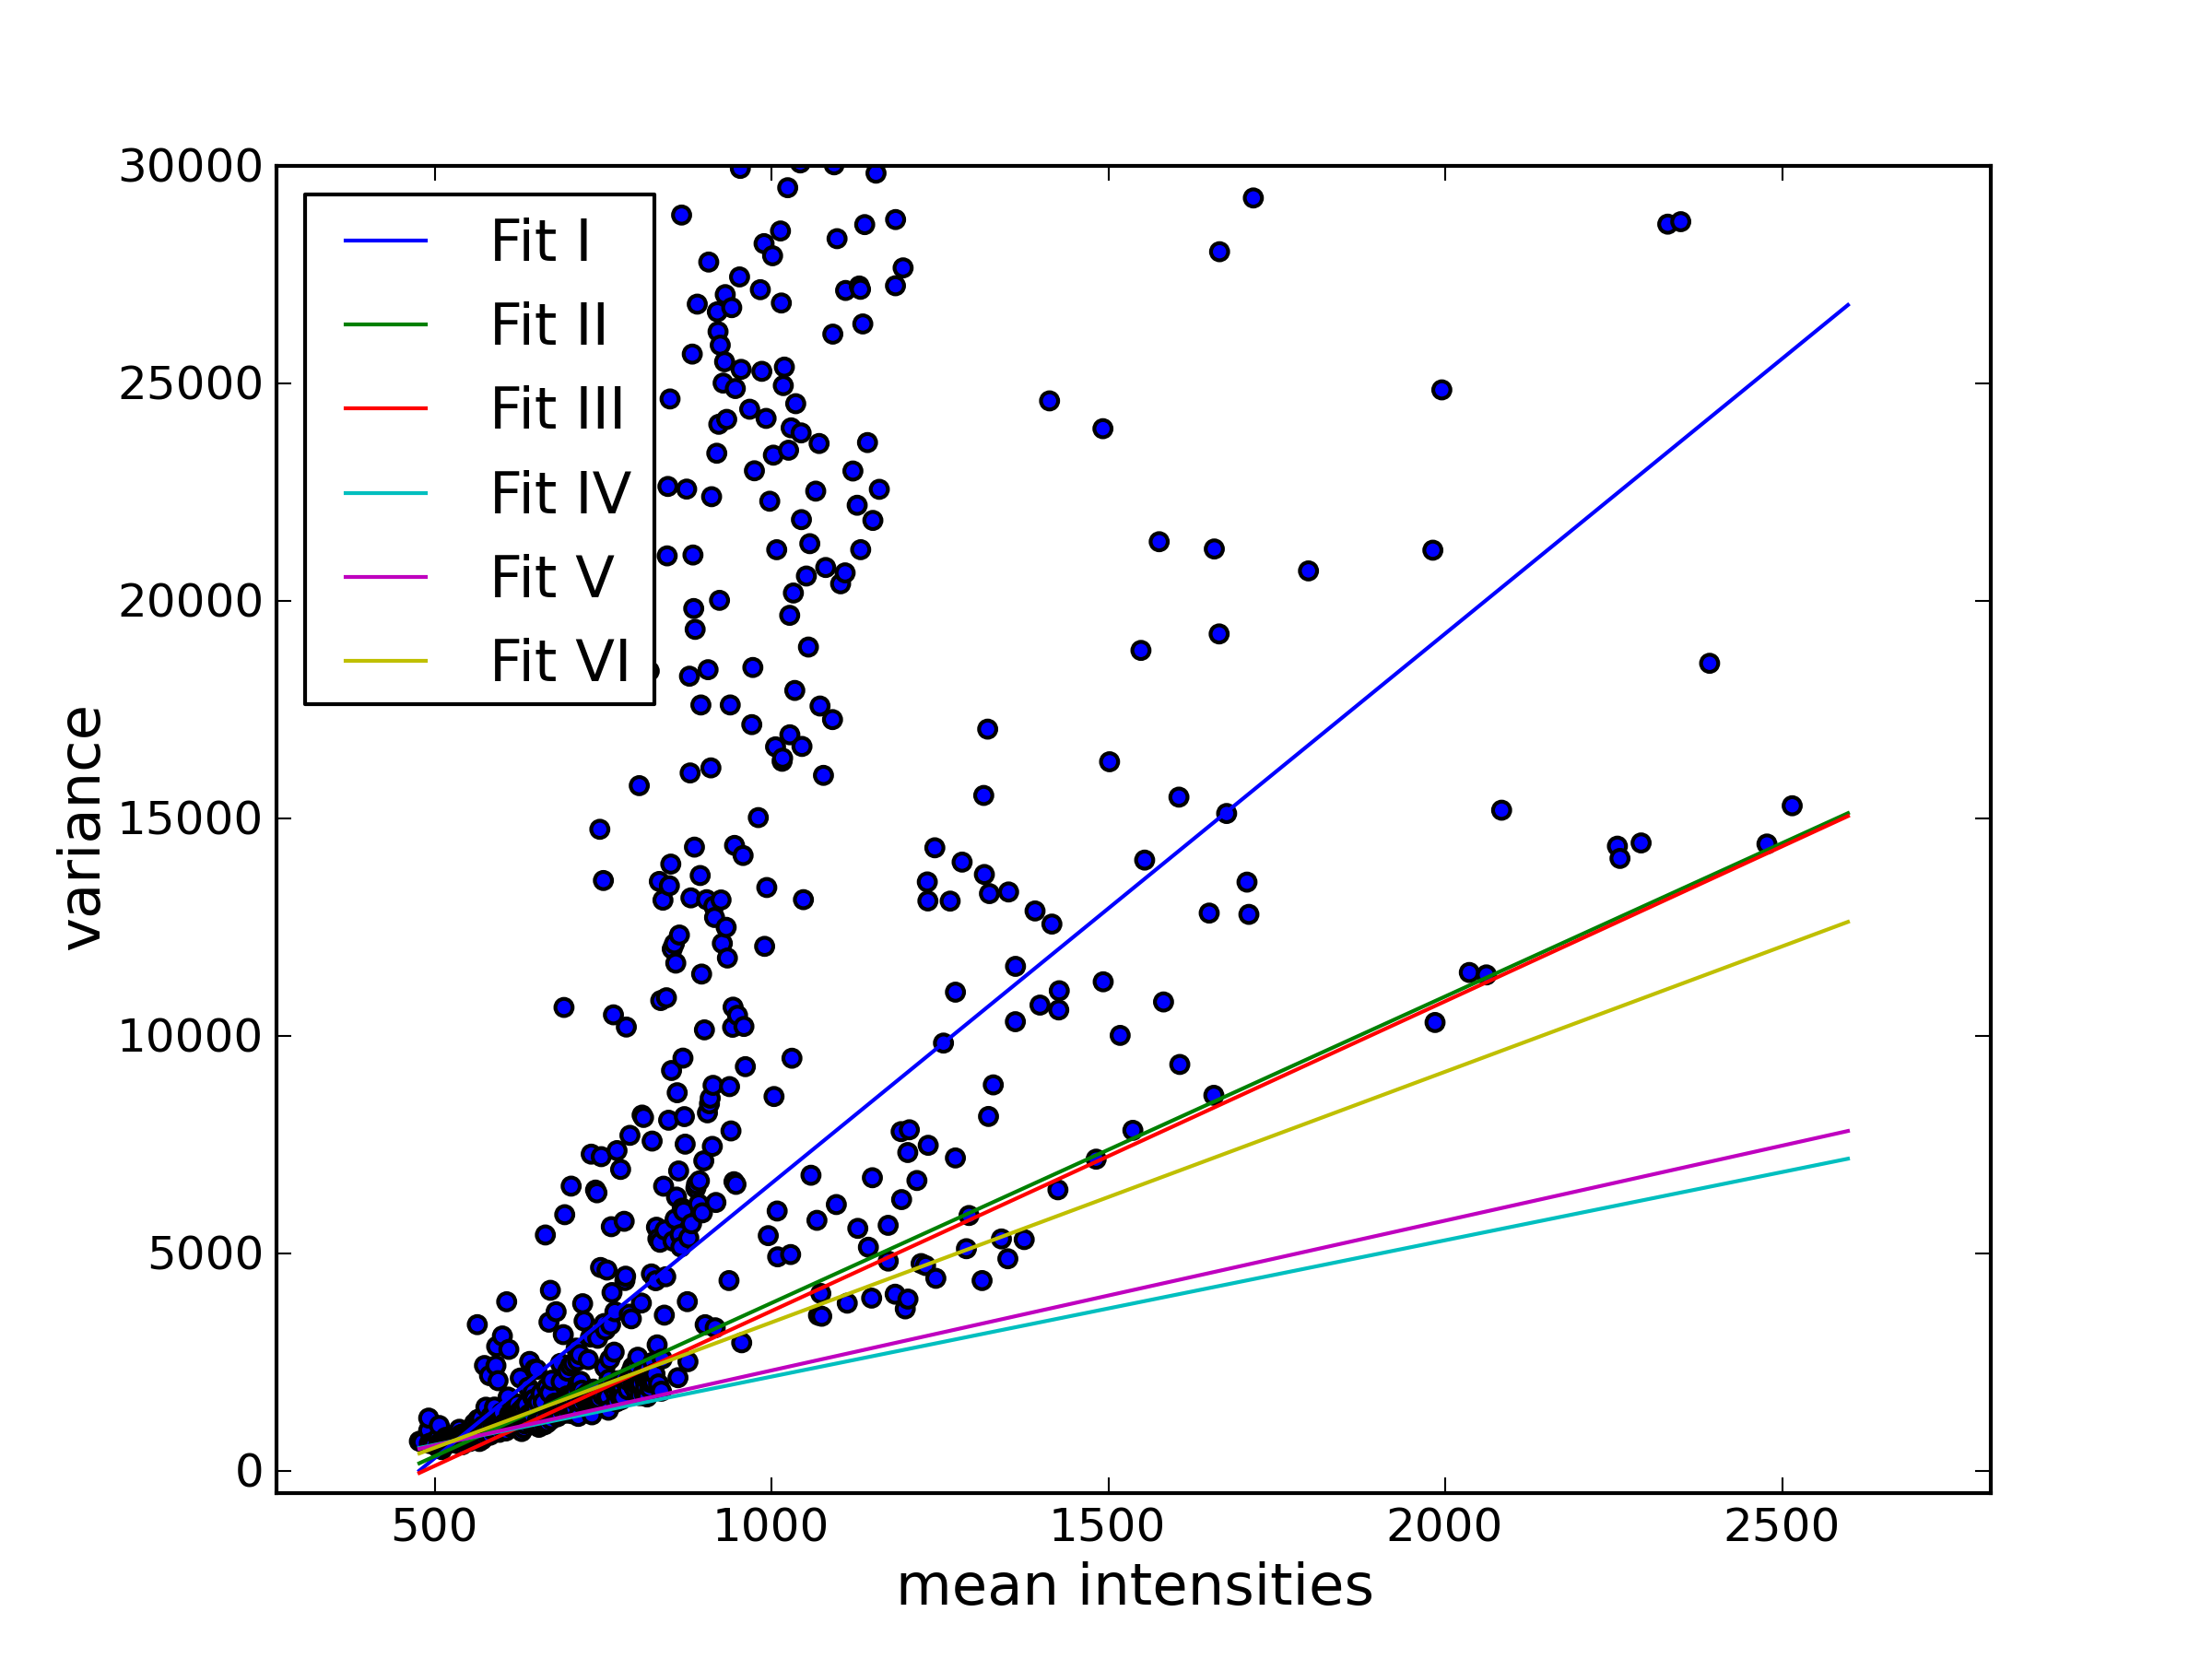
\includegraphics[width =0.48\textwidth]{pictures/geradenplots/pos2green.png}}
\caption{Scatter plot variance over mean for different data sets and the fitting results.}
\label{lineplot1}
\end{figure}

\begin{figure}
\subfloat[Pos2\_2\_red]{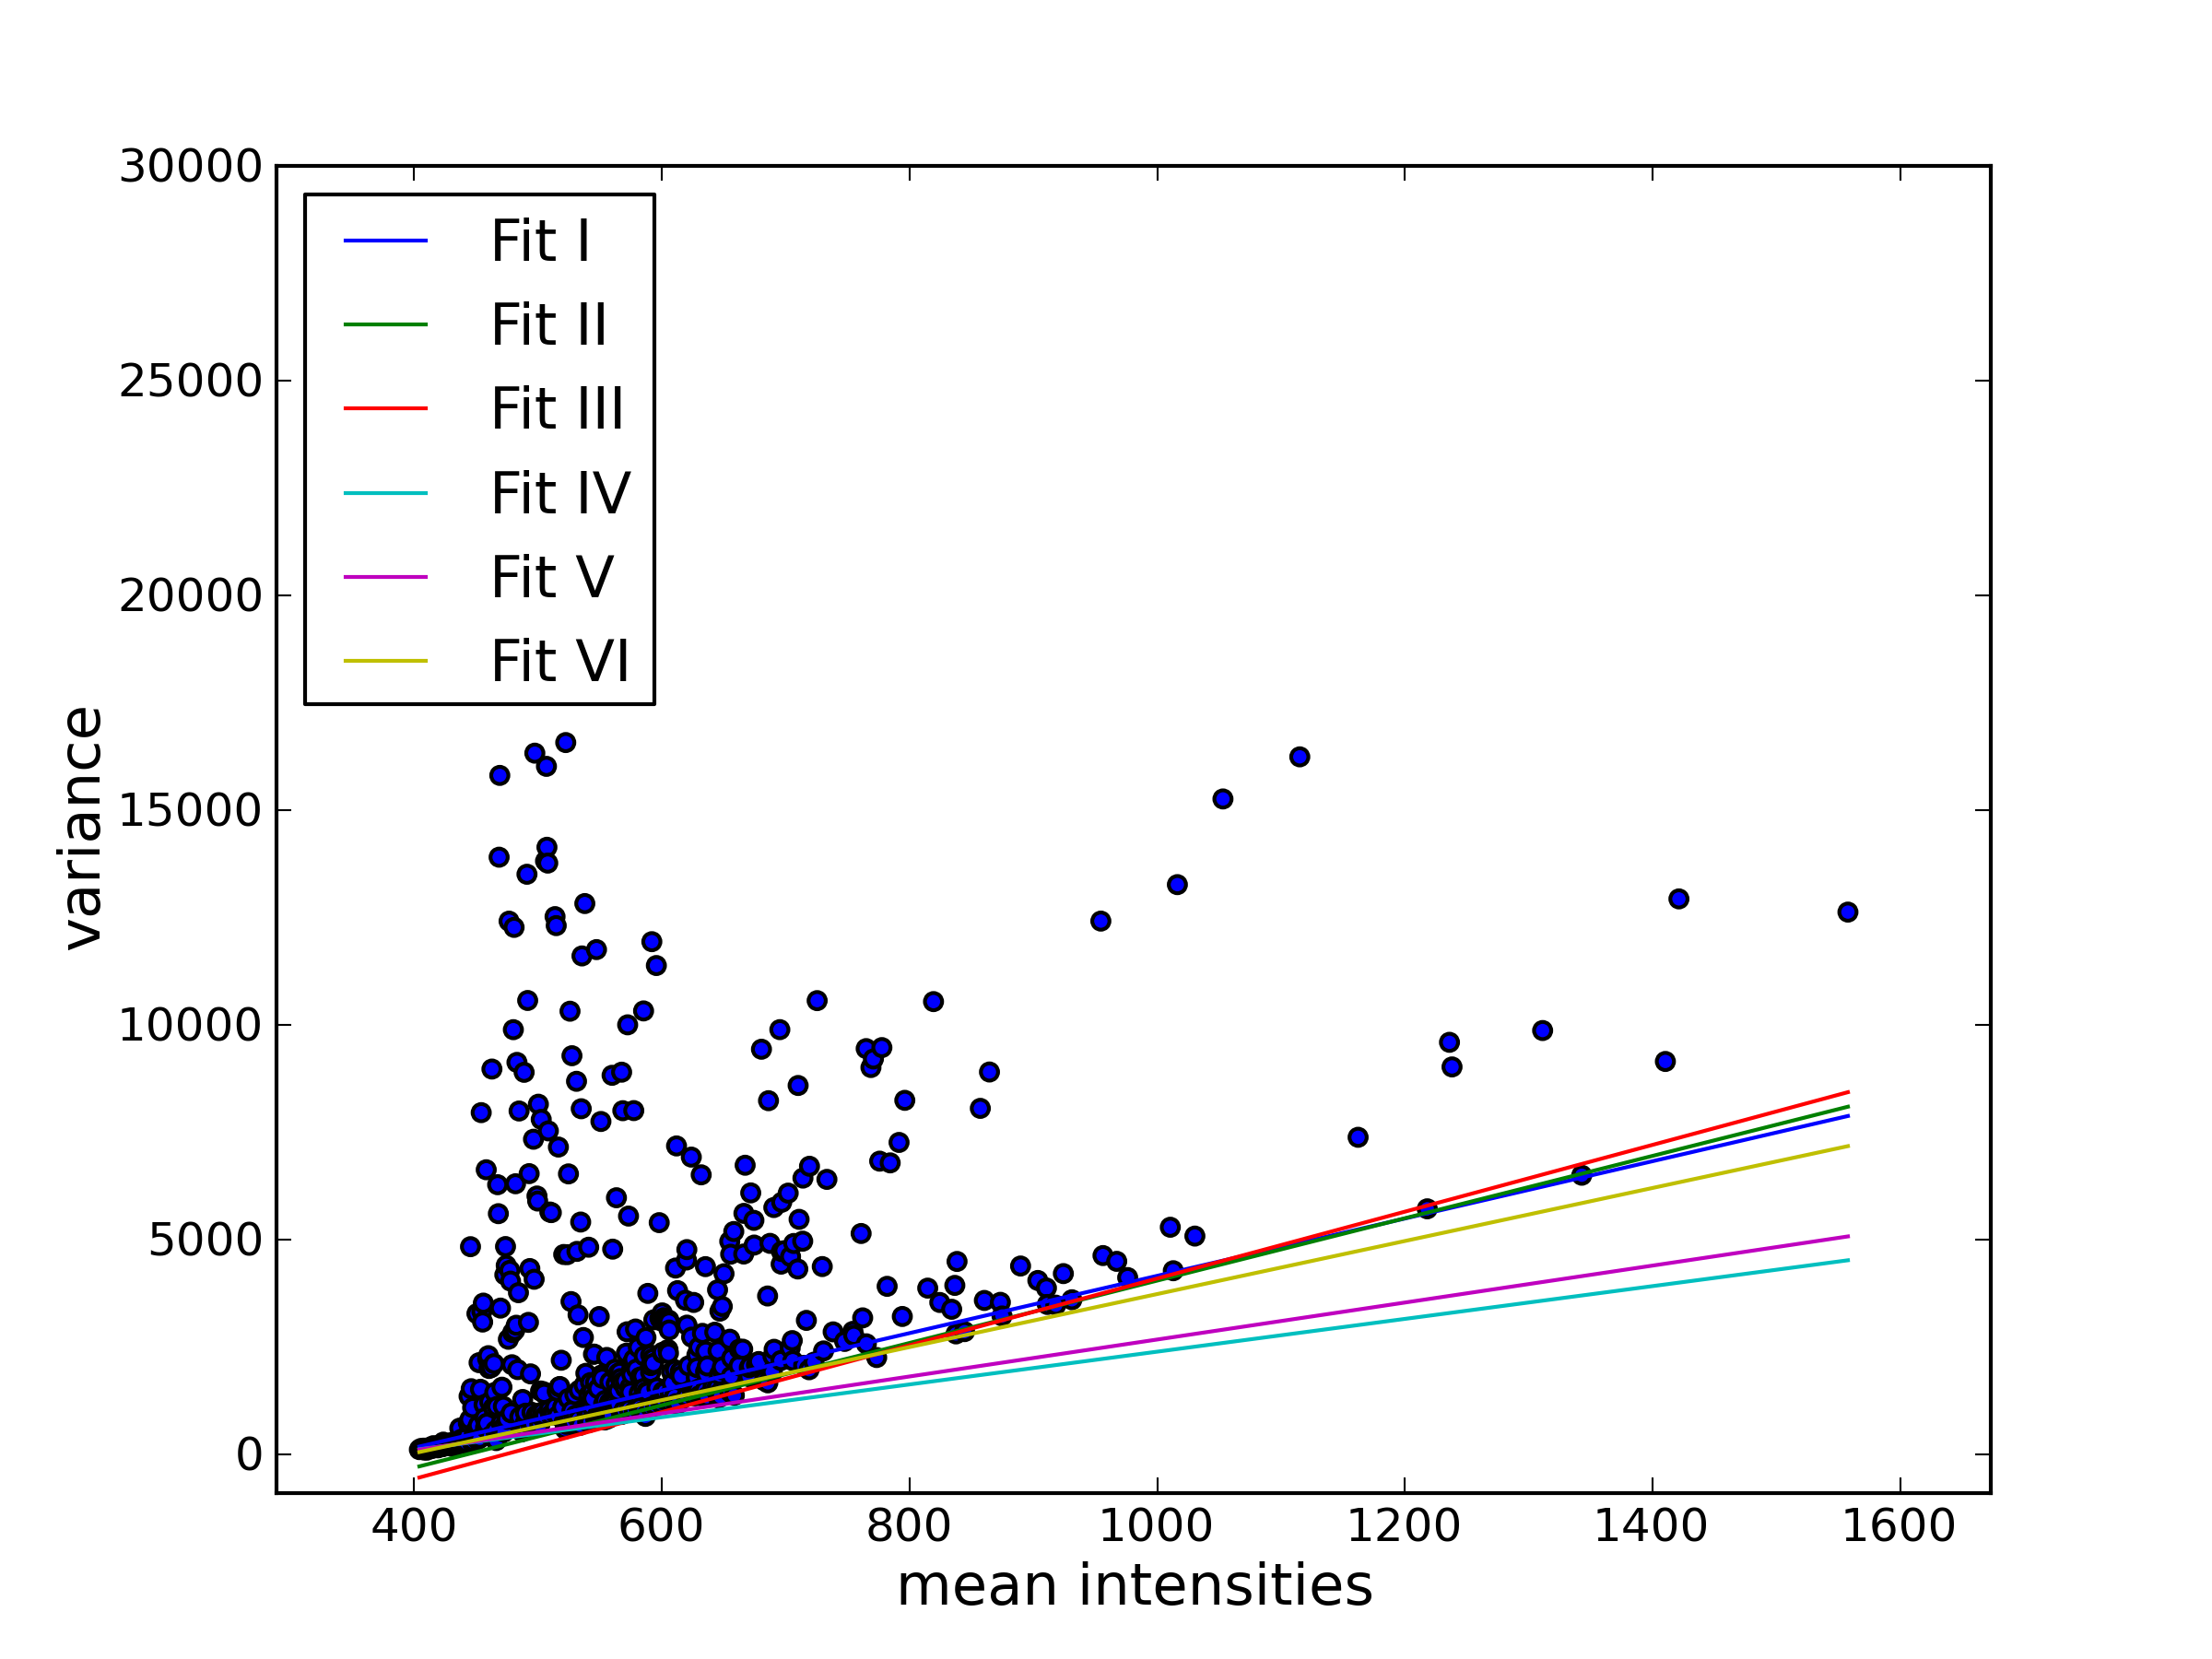
\includegraphics[width =0.48\textwidth]{pictures/geradenplots/pos2red.png}}\hfill
\subfloat[Pos11\_2\_green]{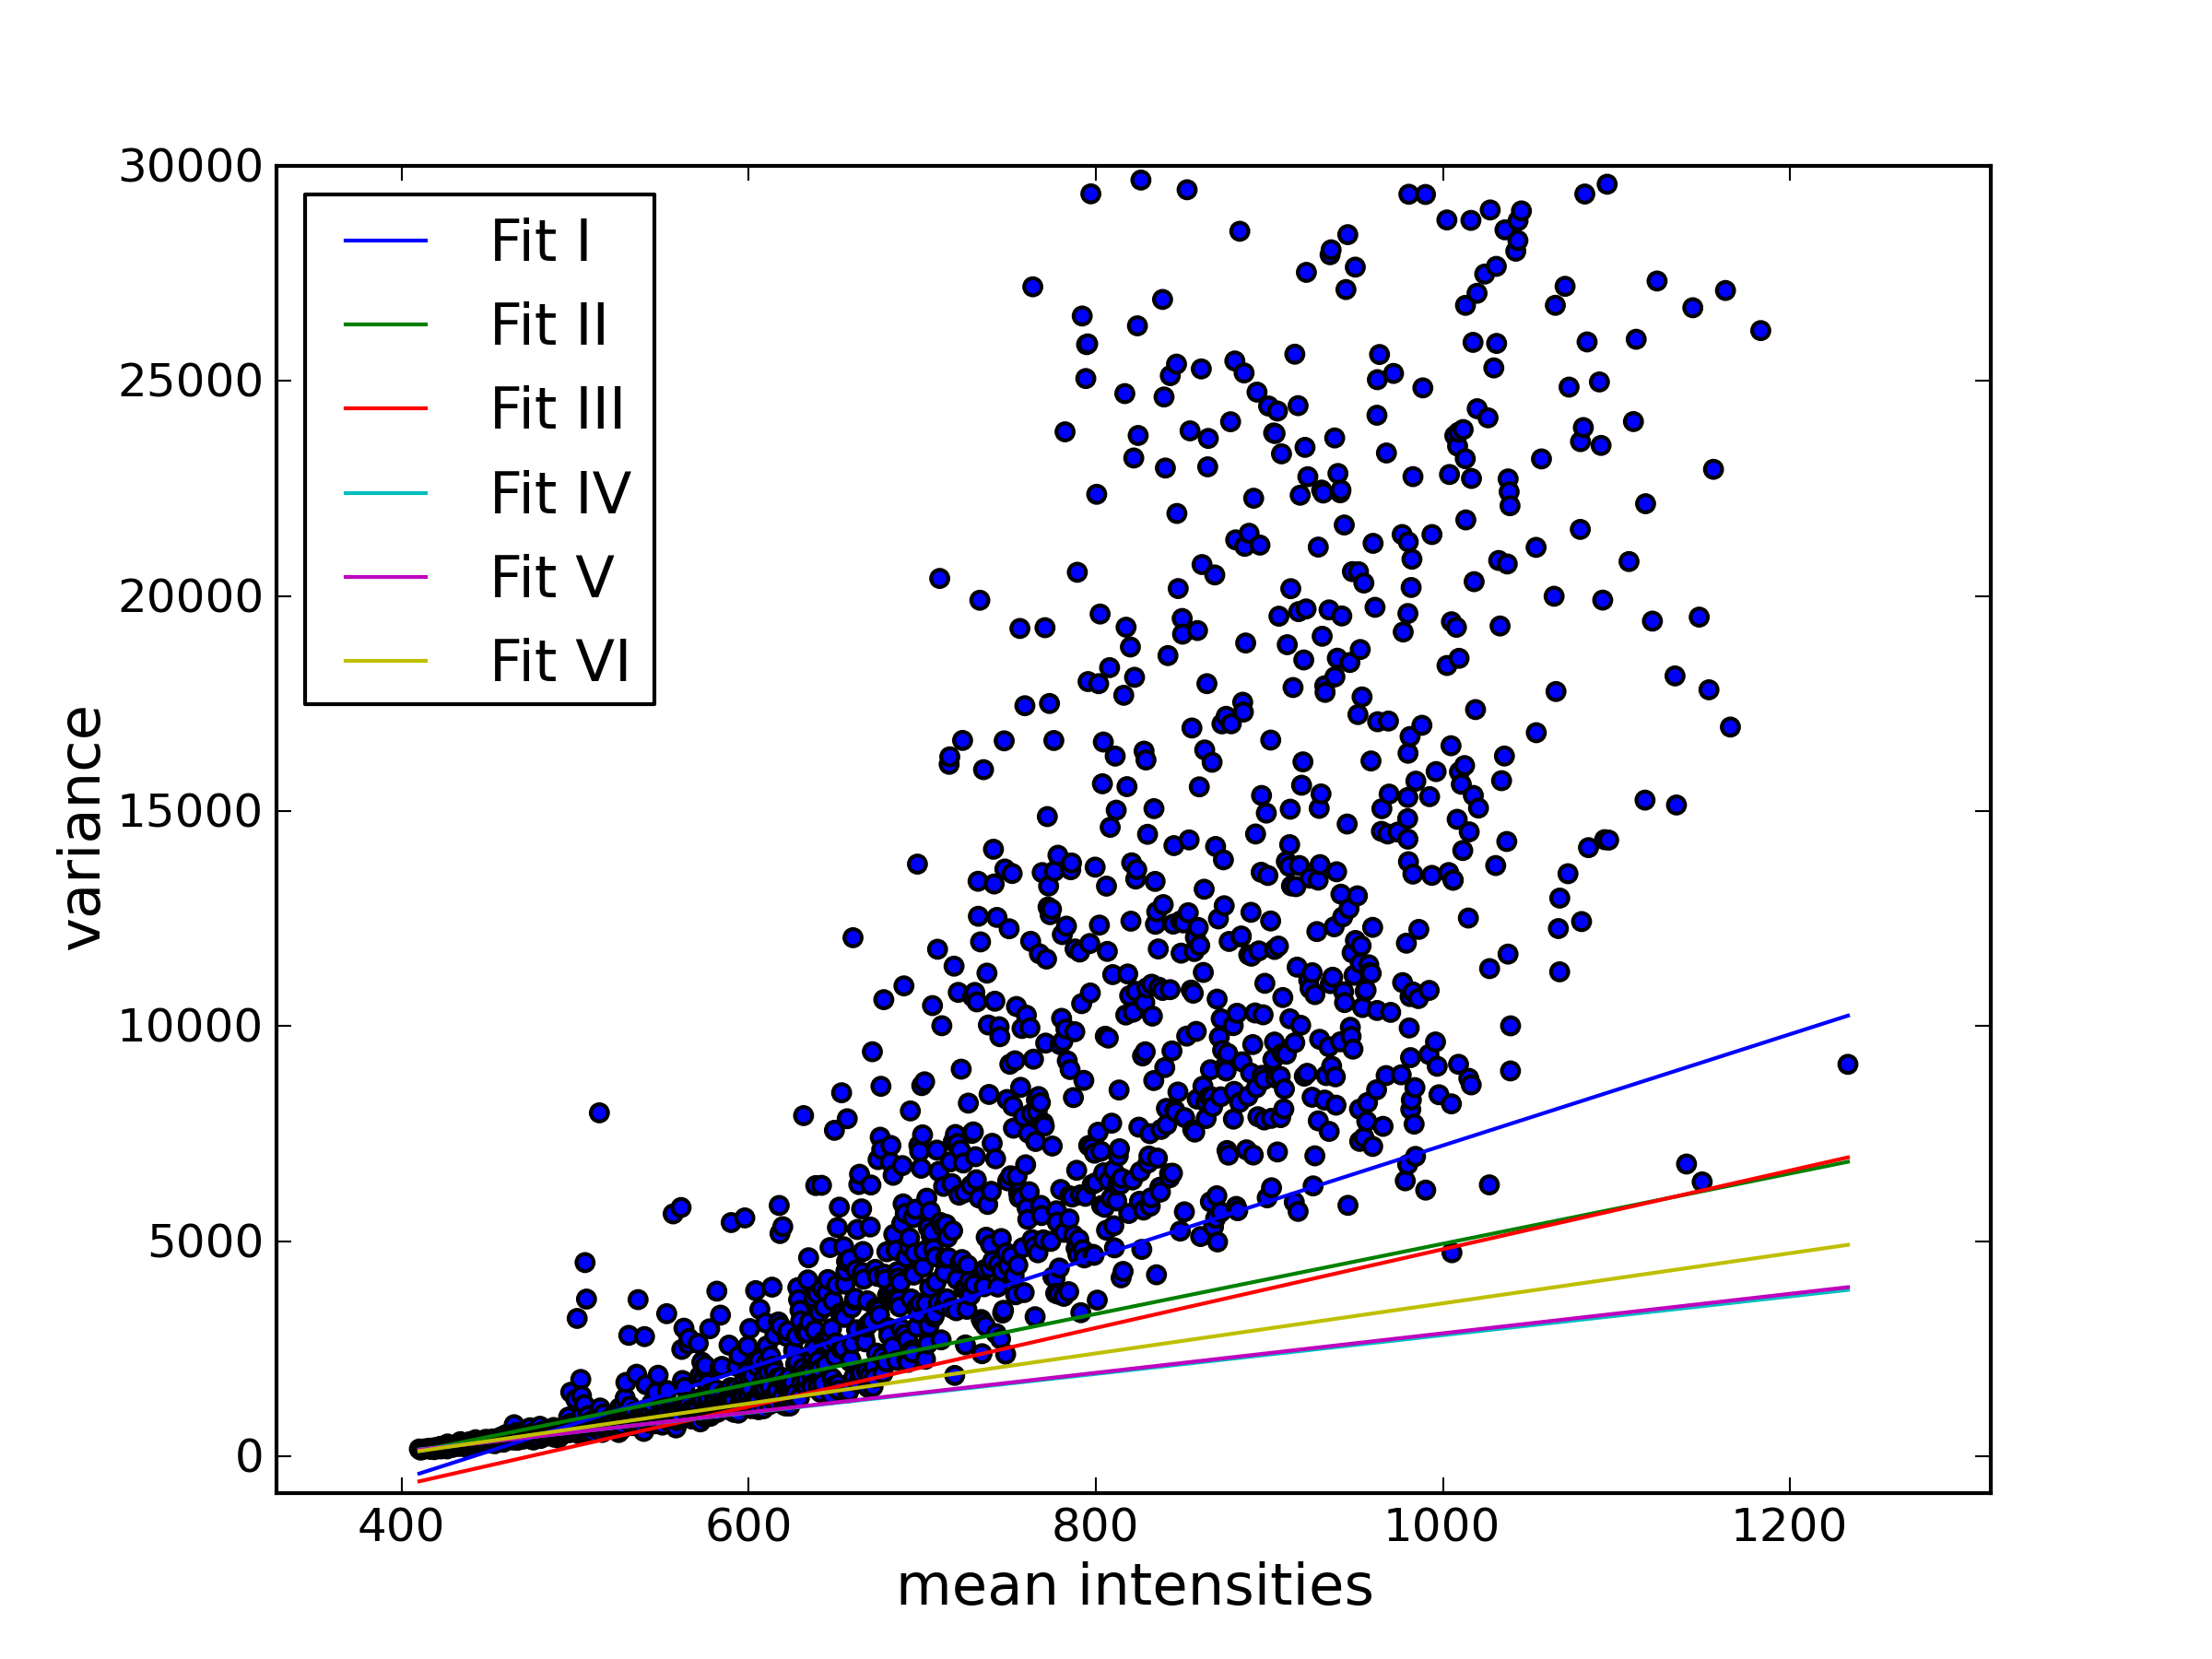
\includegraphics[width =0.48\textwidth]{pictures/geradenplots/pos11green.png}}\hfill
\subfloat[Pos11\_2\_red]{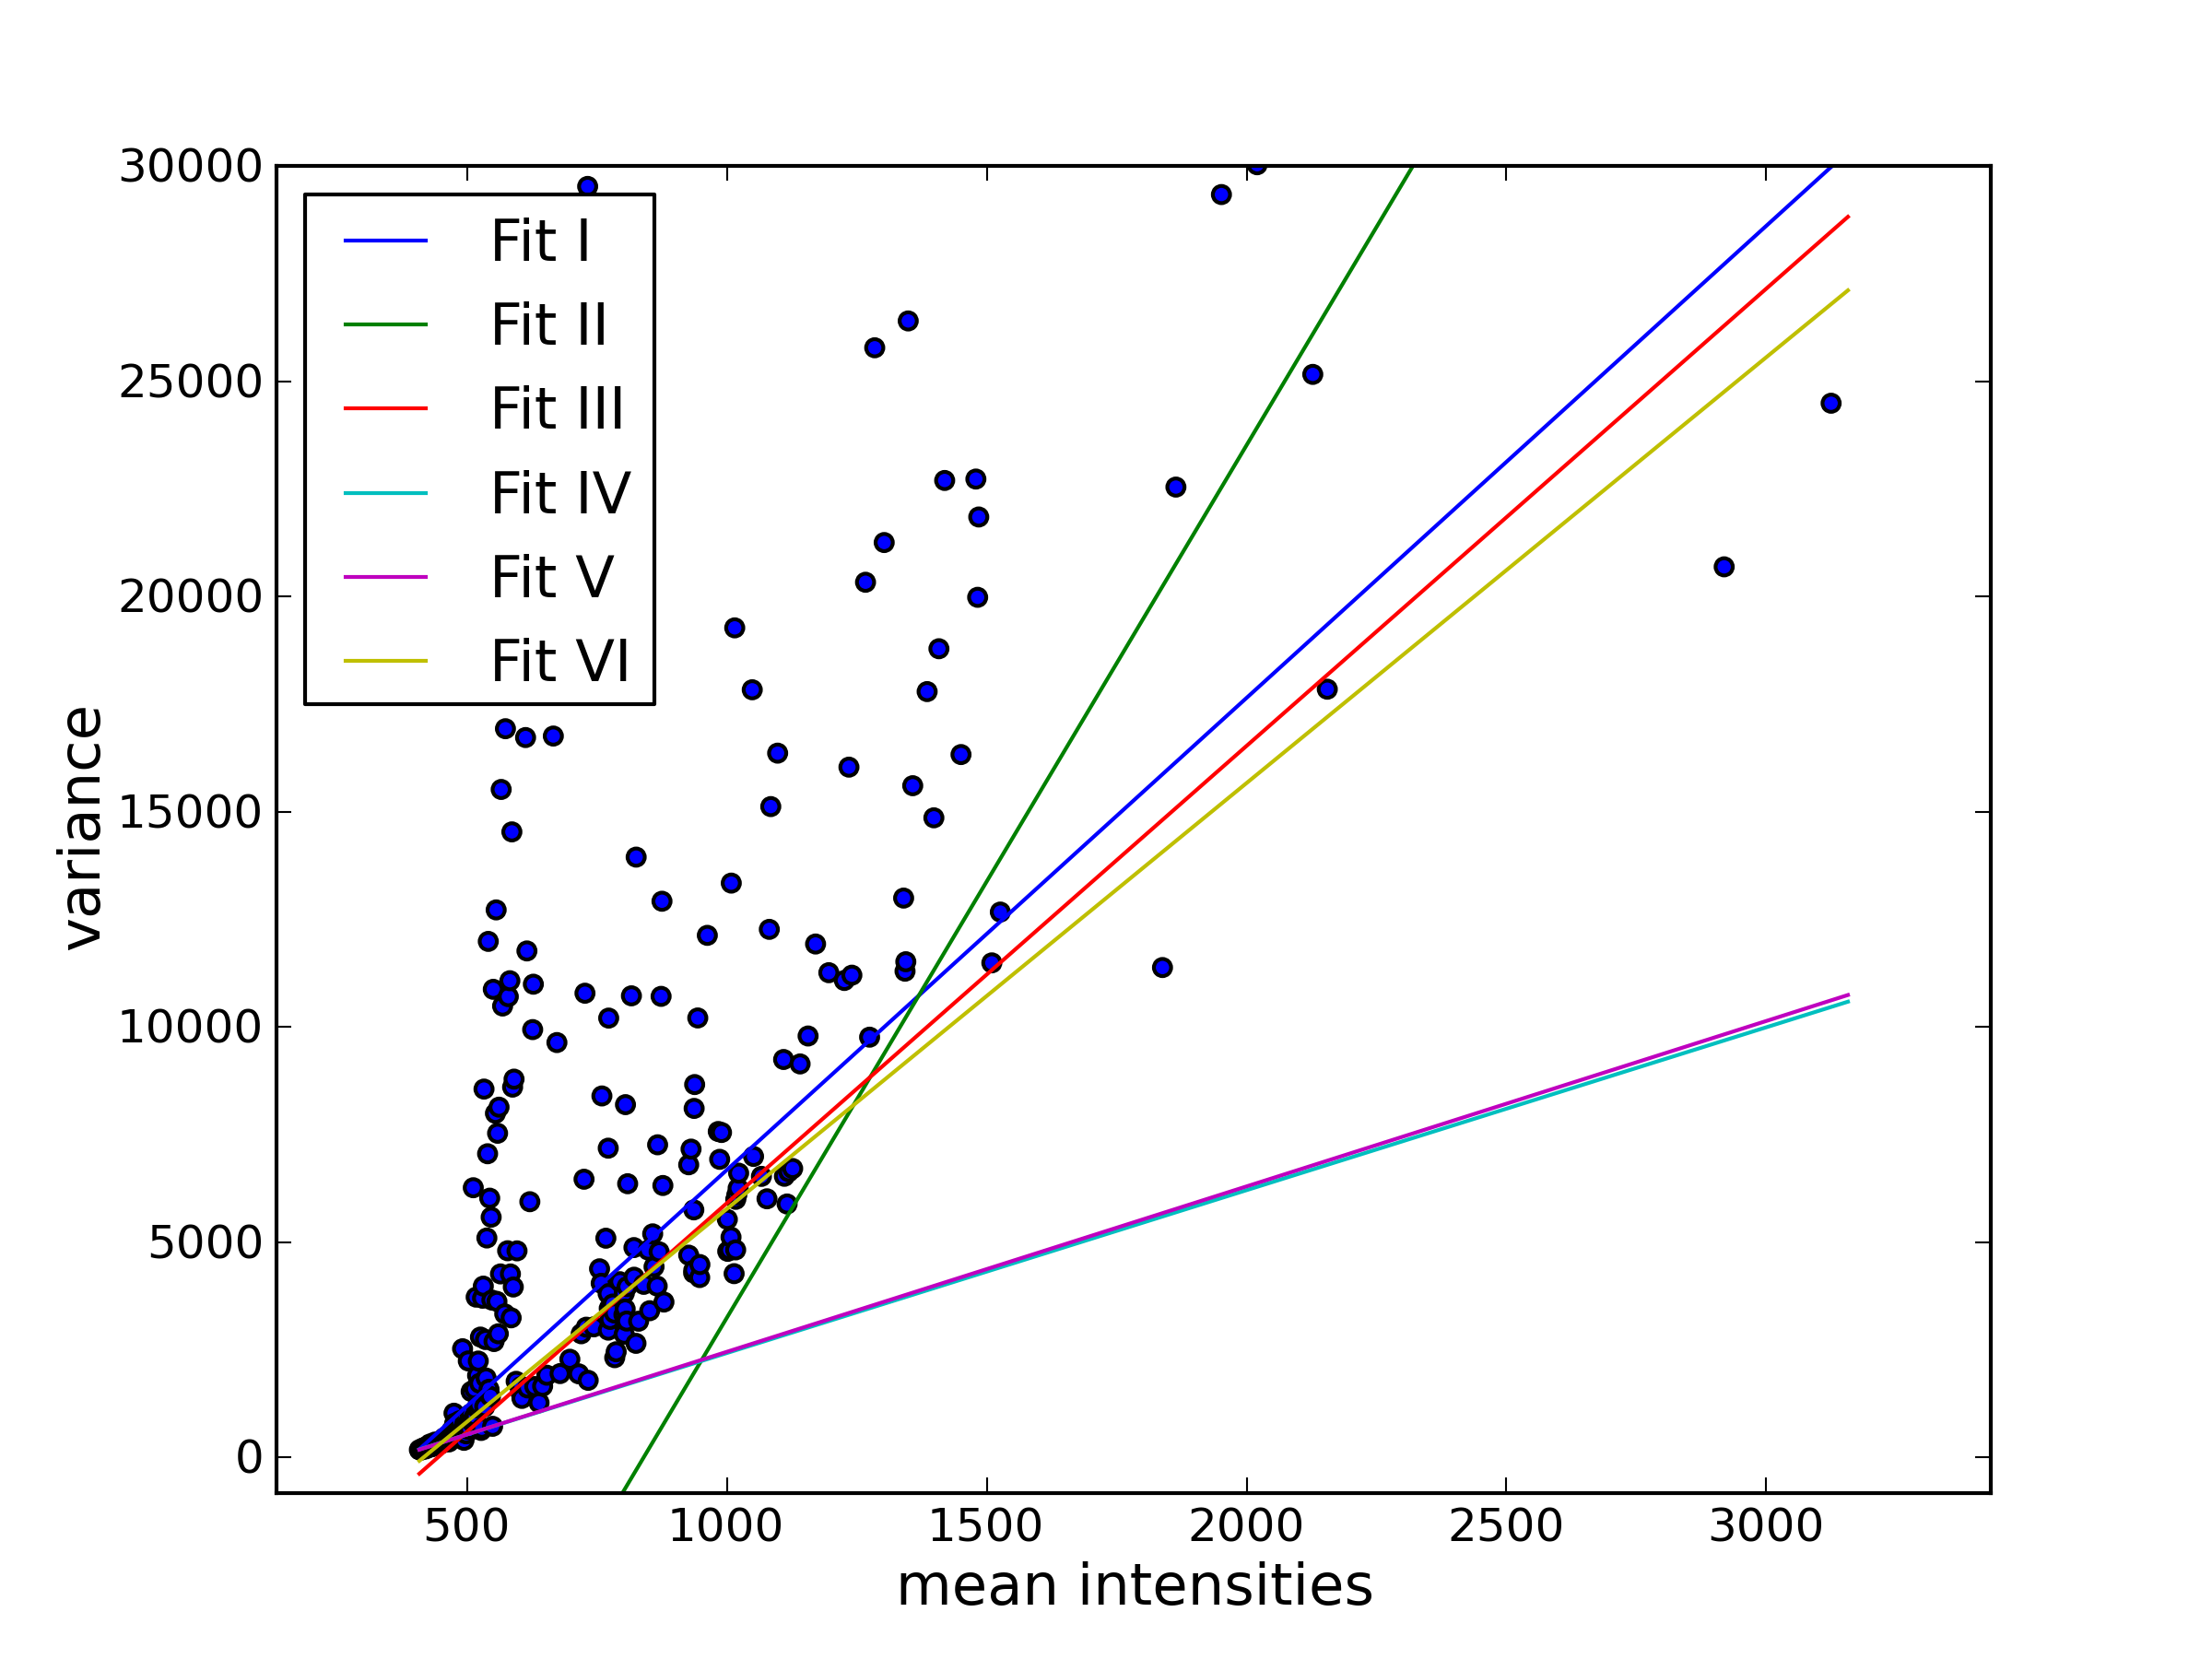
\includegraphics[width =0.48\textwidth]{pictures/geradenplots/pos11red.png}}\hfill
\subfloat[Tetra1\_high\_568]{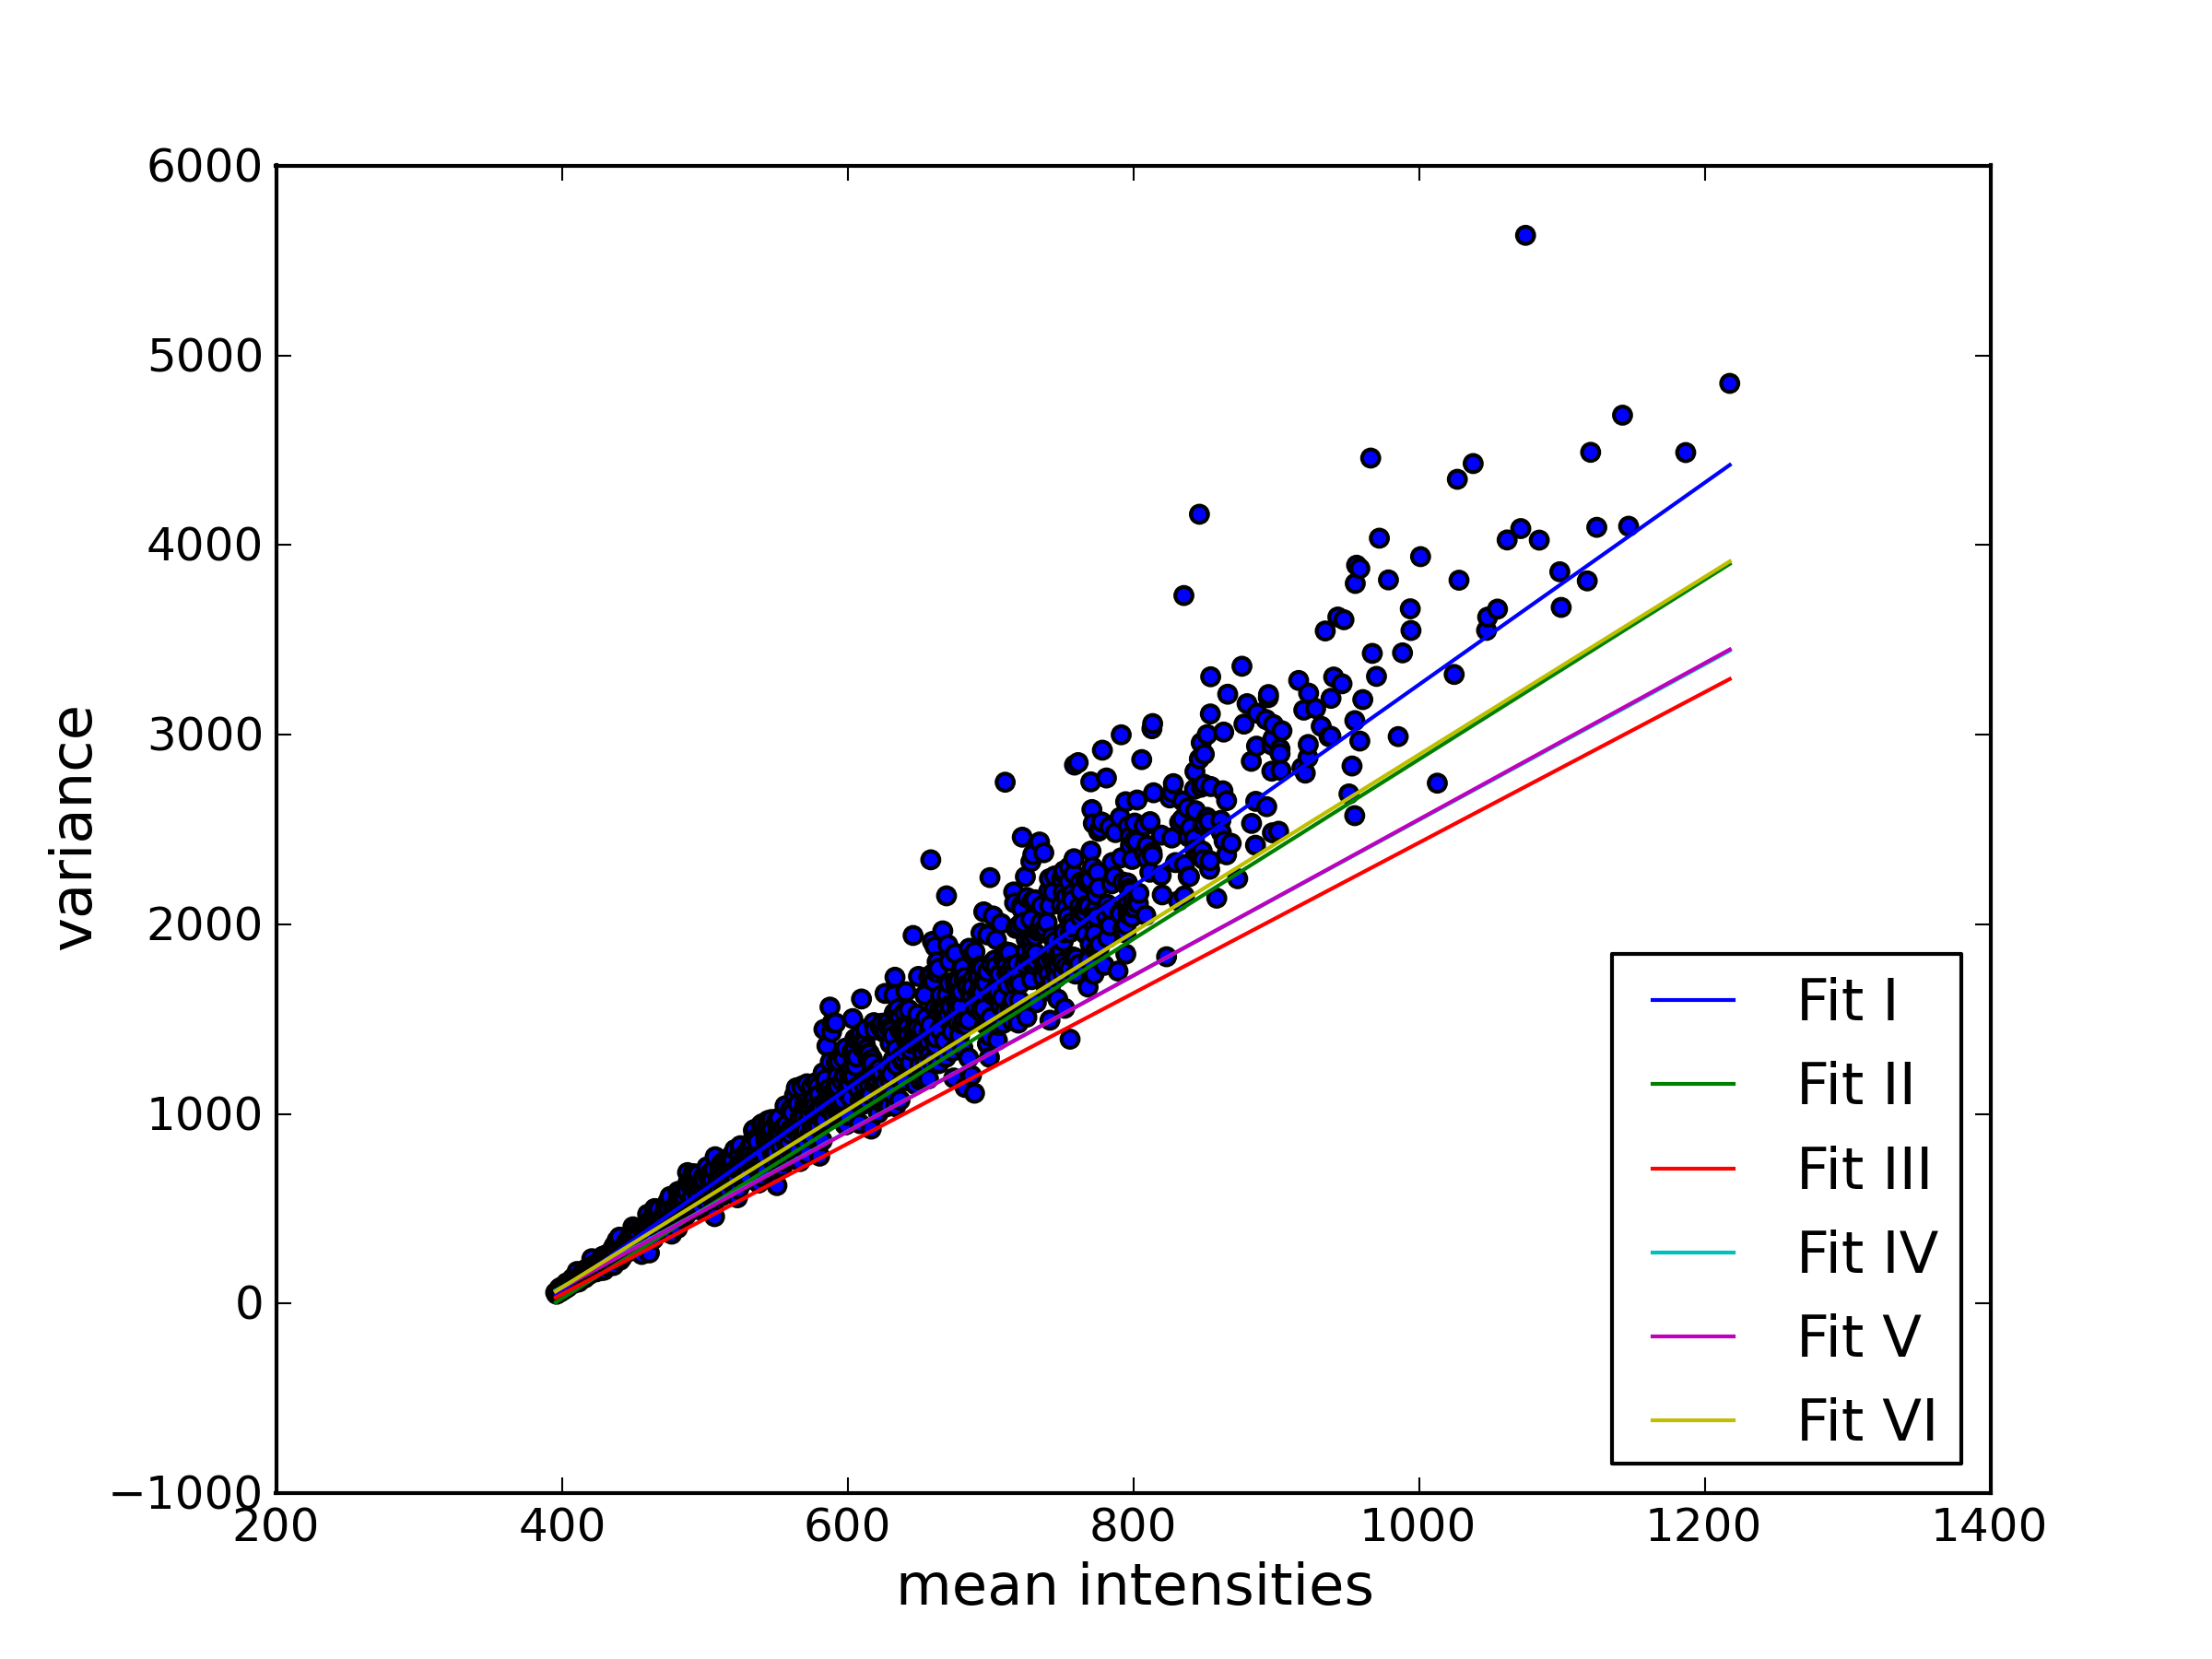
\includegraphics[width =0.48\textwidth]{pictures/geradenplots/tetrahigh568.png}}\\
\subfloat[Tubulin1]{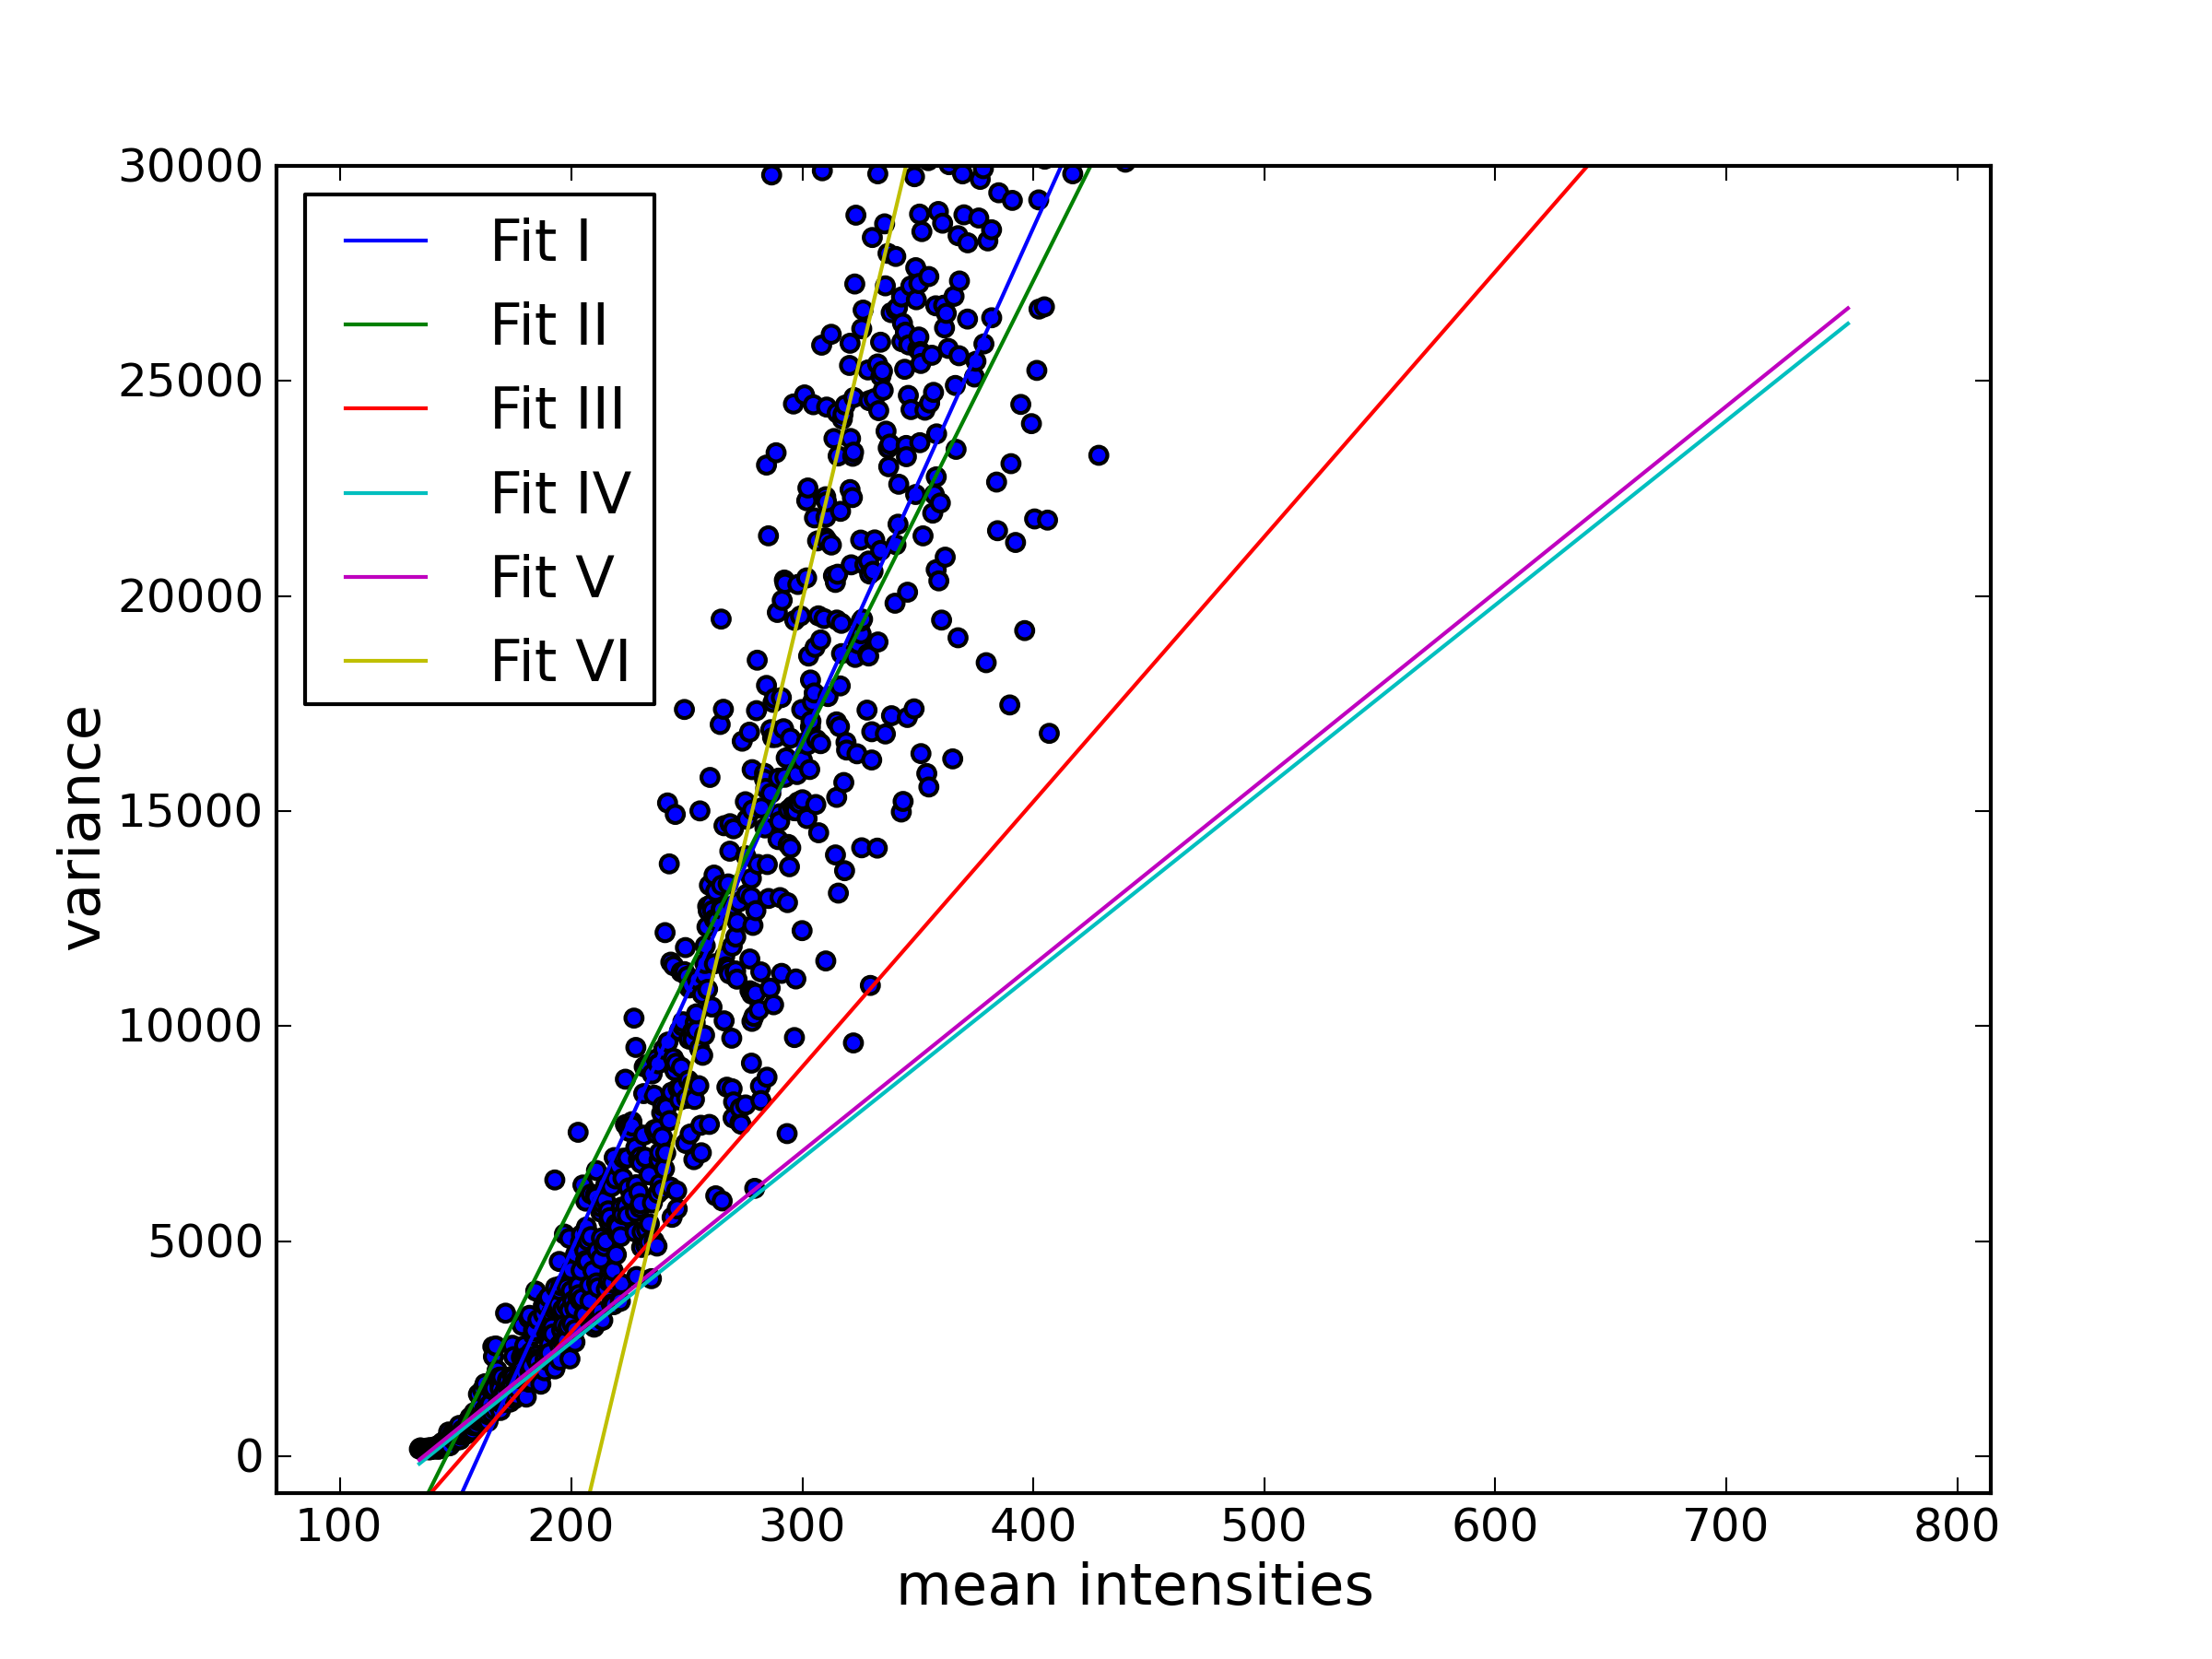
\includegraphics[width =0.48\textwidth]{pictures/geradenplots/bundledtubeshigh.png}}\hfill
\subfloat[Bundled tubes high density]{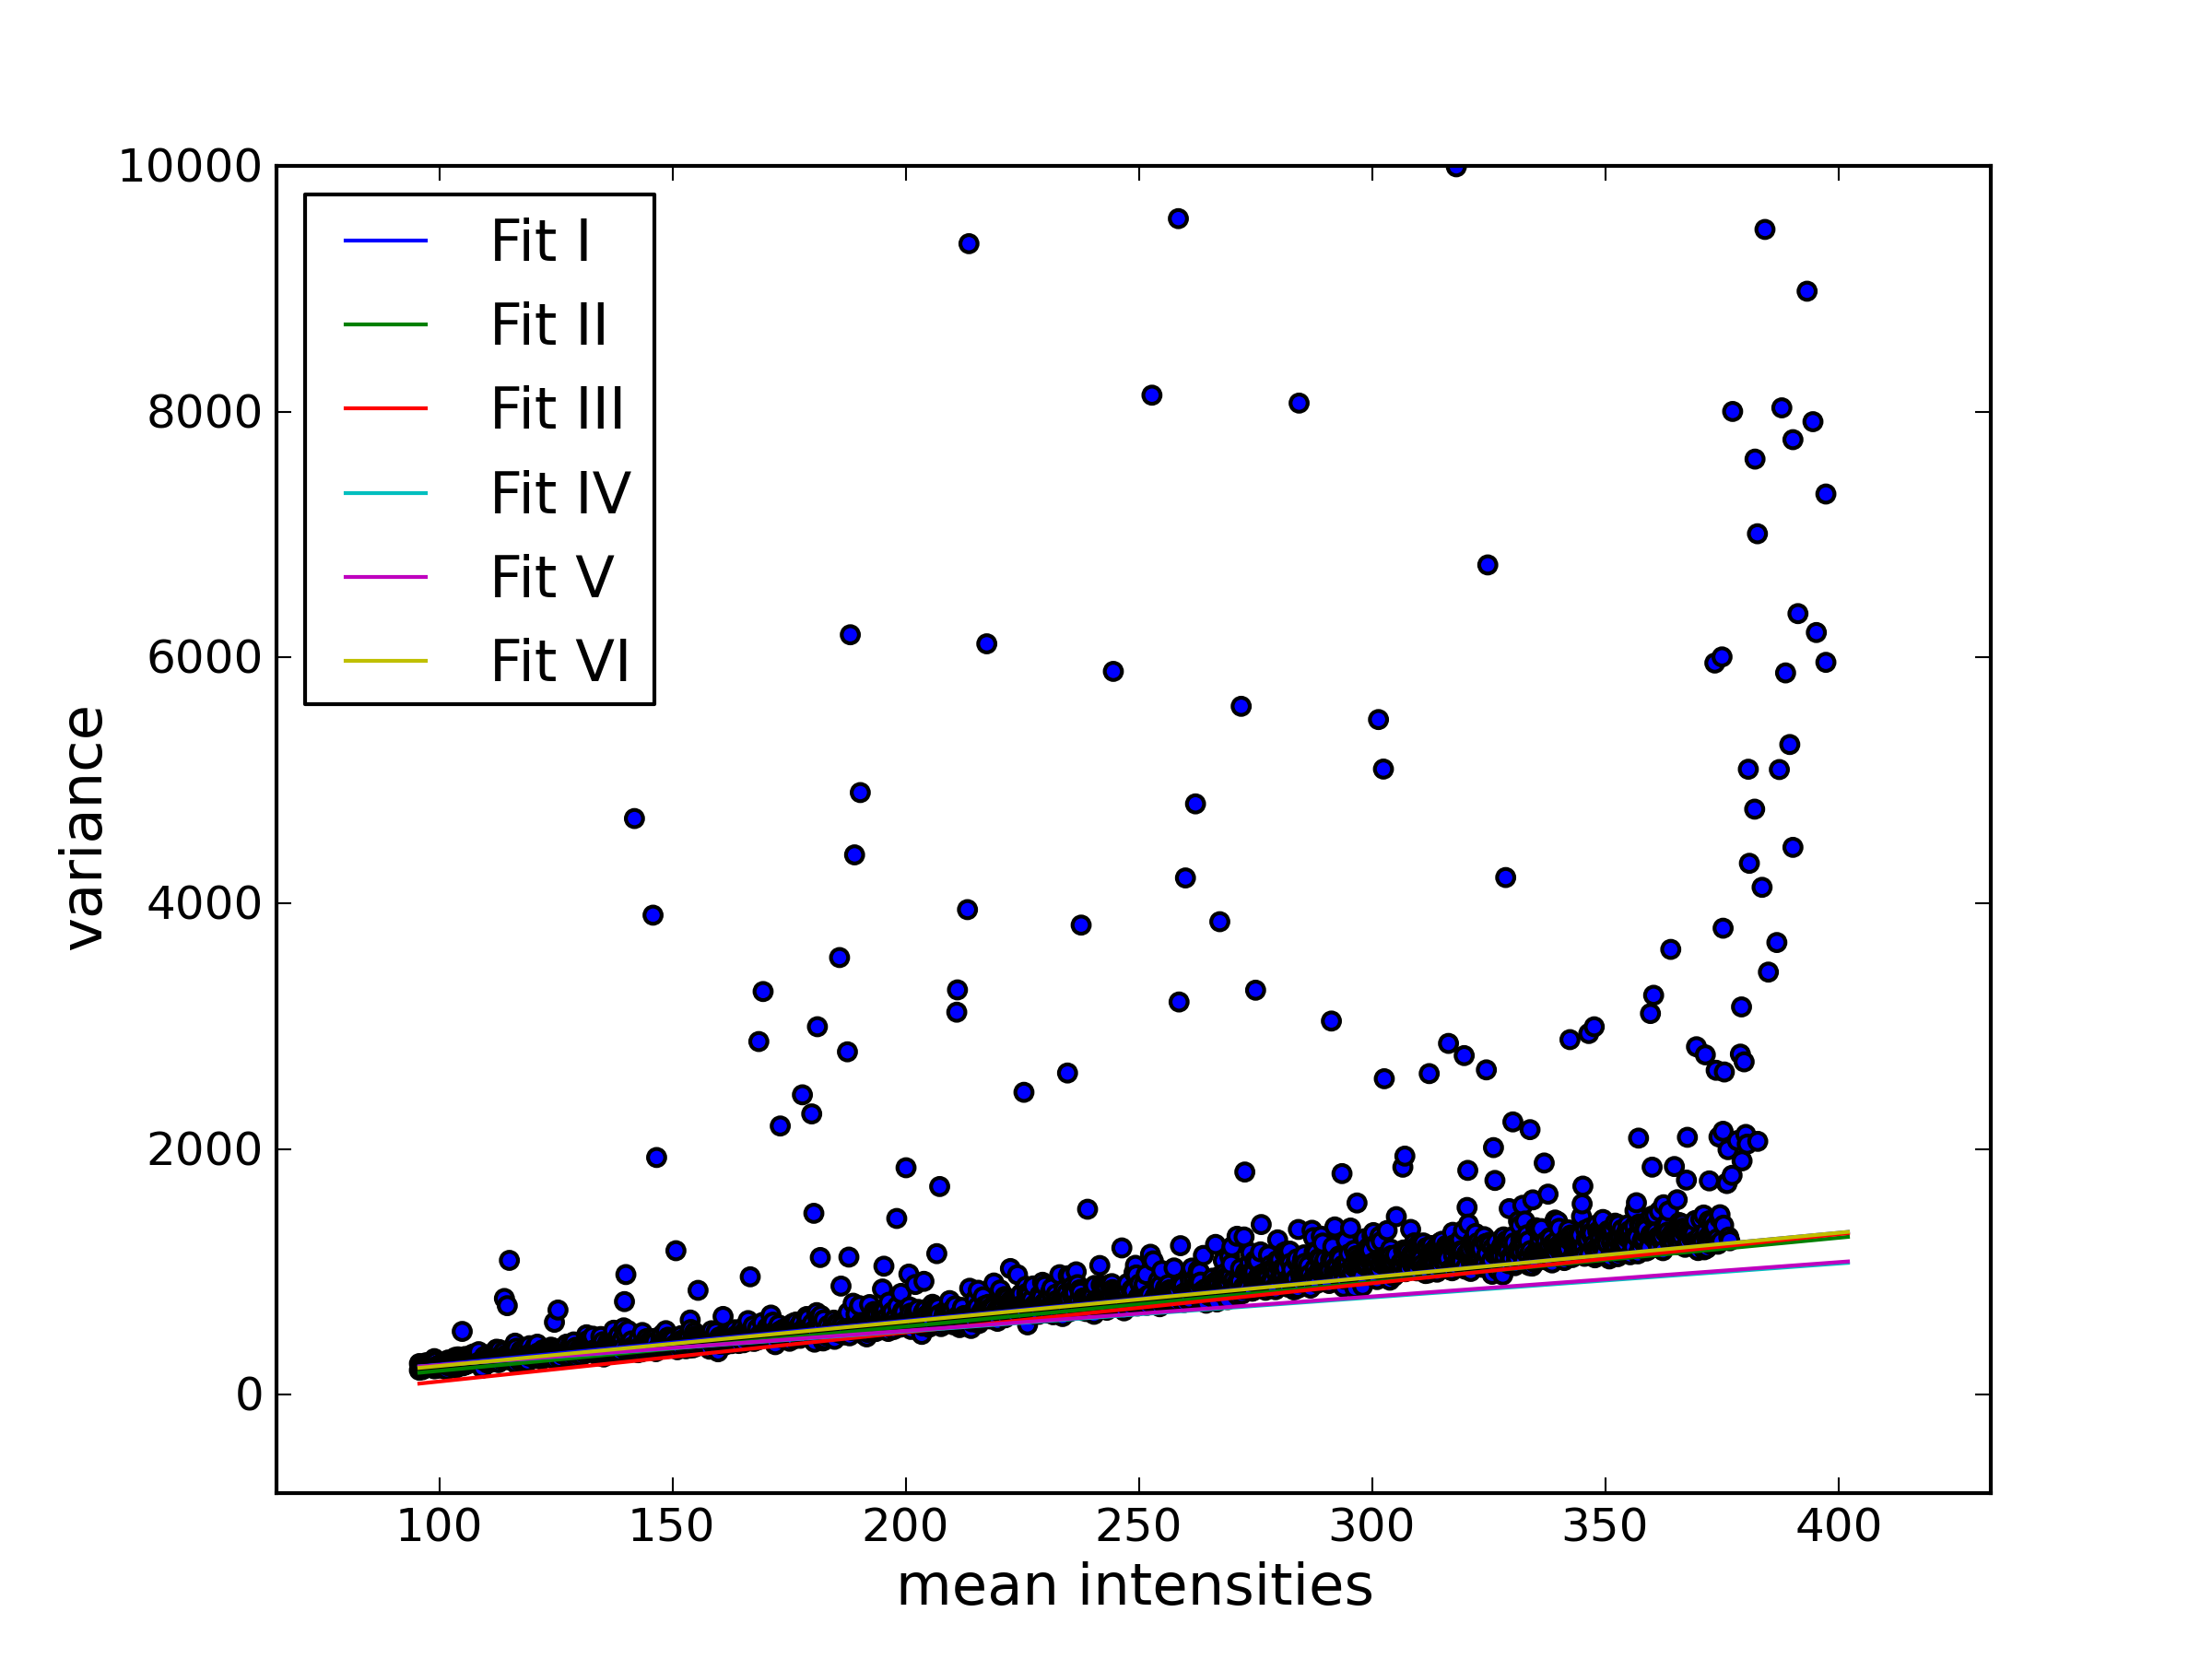
\includegraphics[width =0.48\textwidth]{pictures/geradenplots/tubulin1.png}}
\caption{Scatter plot variance over mean for different data sets and the fitting results.}
\label{lineplot2}
\end{figure}